\documentclass[conference]{IEEEtran}

% =========================================================
% PARÁMETROS CONFIGURABLES POR SEMANA
% =========================================================
\newcommand{\NumeroSemana}{03}
\newcommand{\TemaSemana}{Integración de funciones racionales}

% --- PAQUETES BÁSICOS Y MATEMÁTICOS ---
\usepackage[utf8]{inputenc}
\usepackage[T1]{fontenc}
\usepackage{amsmath,amssymb,amsfonts}
\usepackage{mathtools}
\usepackage{graphicx}
\usepackage{hyperref}
\usepackage{float}
\usepackage{array}

% --- RUTA BÁSICA DE IMÁGENES ---
\graphicspath{{semana_03/graficas/}}

\begin{document}
	
	% =========================================================
	% PORTADA OFICIAL FORMATO IEEE - FIEE UNMSM
	% =========================================================
	\title{UNIVERSIDAD NACIONAL MAYOR DE SAN MARCOS\\
		\Large FACULTAD DE INGENIERÍA ELECTRÓNICA Y ELÉCTRICA (FIEE)\\
		\vspace{0.3cm}
		\large \textbf{Curso:} Cálculo II (Cálculo Integral) \quad|\quad \textbf{Docente:} Dr. Raúl Castro Vidal\\
		\vspace{0.4cm}
		\huge SOLUCIÓN DE EJERCICIOS PROPUESTOS --- SEMANA \NumeroSemana\\
		\LARGE INFORME TÉCNICO GRUPAL: \TemaSemana}
	
	% --- BLOQUE DE AUTORES ---
\author{
	\IEEEauthorblockN{Coordinador: Adrián Córdova Suazo}
	\IEEEauthorblockA{\textit{Código: 26190164} \\
		\textit{Ing. Electrónica}}
	\and
	\IEEEauthorblockN{Integrante 2: Diego Checcori Cuya}
	\IEEEauthorblockA{\textit{Código: 26190008} \\
		\textit{Ing. Electrónica}}
	\and
	\IEEEauthorblockN{Integrante 3: Diego Anamaria Choque}
	\IEEEauthorblockA{\textit{Código: 26190001} \\
		\textit{Ing. Electrónica}}
	\vspace{0.4cm}
	\and
	\IEEEauthorblockN{Integrante 4: Deyvis Tenorio Yucra}
	\IEEEauthorblockA{\textit{Código: 26190199} \\
		\textit{Ing. Electrónica}}
	\and
	\IEEEauthorblockN{Integrante 5: Felix Chocce Oseda}
	\IEEEauthorblockA{\textit{Código: 23190231} \\
		\textit{Ing. Eléctrica}}
	\and
	\IEEEauthorblockN{Integrante 6: Isaac Guadalupe Baños}
	\IEEEauthorblockA{\textit{Código: 26190169} \\
		\textit{Ing. Electrónica}}
}

\maketitle
	
	\begin{abstract}
		En el presente informe técnico correspondiente a la asignatura de Cálculo II, a cargo del Dr. Raúl Castro Vidal, se presenta la solución analítica paso a paso de los ejercicios propuestos para la Semana \NumeroSemana. Cada problema incluye su representación y análisis gráfico desarrollado en Matplotlib evaluado en la constante de integración $C=0$, estructurado formalmente bajo los estándares IEEE a dos columnas.
	\end{abstract}
	
	\begin{IEEEkeywords}
		Cálculo II, \TemaSemana, Matplotlib, Formato IEEE, FIEE-UNMSM.
	\end{IEEEkeywords}
	
	\section{Desarrollo de los Ejercicios}
	
	% --- LISTA DIRECTA CON RUTAS EXPLÍCITAS ---
	\subsection*{Problema 01}

\noindent \textbf{Enunciado:} \\
Calcular la integral indefinida:
\begin{align*}
\int \dfrac{dx}{4x^2 + 4x + 10}
\end{align*}

\noindent \textbf{Solución:} \\
Primero, analizamos el denominador de la función integranda. Completamos el trinomio cuadrado perfecto agrupando los términos en $x$:
\begin{align*}
4x^2 + 4x + 10 &= 4\left(x^2 + x\right) + 10
\end{align*}

\noindent Completamos el cuadrado dentro del paréntesis sumando y restando $\left(\frac{1}{2}\right)^2 = \frac{1}{4}$:
\begin{align*}
4x^2 + 4x + 10 &= 4\left(x^2 + x + \dfrac{1}{4} - \dfrac{1}{4}\right) + 10 \\
&= 4\left(x + \dfrac{1}{2}\right)^2 - 1 + 10 \\
&= 4\left(x + \dfrac{1}{2}\right)^2 + 9
\end{align*}

\noindent Sustituimos esta expresión equivalente en el denominador de la integral original:
\begin{align*}
\int \dfrac{dx}{4x^2 + 4x + 10} &= \int \dfrac{dx}{4\left(x + \frac{1}{2}\right)^2 + 9}
\end{align*}

\noindent Para resolver esta integral, aplicamos la sustitución trigonométrica sugerida o un cambio de variable lineal. Sea:
\begin{align*}
u &= x + \dfrac{1}{2}, \quad du = dx
\end{align*}

\noindent La integral se transforma en:
\begin{align*}
\int \dfrac{du}{4u^2 + 9} &= \int \dfrac{du}{9 \left(\left(\frac{2}{3}u\right)^2 + 1\right)}
\end{align*}

\noindent Hacemos un segundo cambio de variable con $w = \frac{2}{3}u$, de donde $dw = \frac{2}{3}du$, lo que implica $du = \frac{3}{2}dw$:
\begin{align*}
&= \dfrac{1}{9} \int \dfrac{\frac{3}{2} dw}{w^2 + 1} \\
&= \dfrac{3}{18} \int \dfrac{dw}{w^2 + 1} \\
&= \dfrac{1}{6} \arctan(w) + C
\end{align*}

\noindent Retornando a la variable original $u$ y posteriormente a $x$:
\begin{align*}
&= \dfrac{1}{6} \arctan\left(\dfrac{2}{3}u\right) + C \\
&= \dfrac{1}{6} \arctan\left[\dfrac{2}{3}\left(x + \dfrac{1}{2}\right)\right] + C \\
&= \dfrac{1}{6} \arctan\left(\dfrac{2x + 1}{3}\right) + C
\end{align*}

\noindent Por lo tanto, el resultado de la integral indefinida es:
\begin{align*}
\int \dfrac{dx}{4x^2 + 4x + 10} = \dfrac{1}{6} \arctan\left(\dfrac{2x + 1}{3}\right) + C
\end{align*}

\begin{figure}[H]
	\centering
	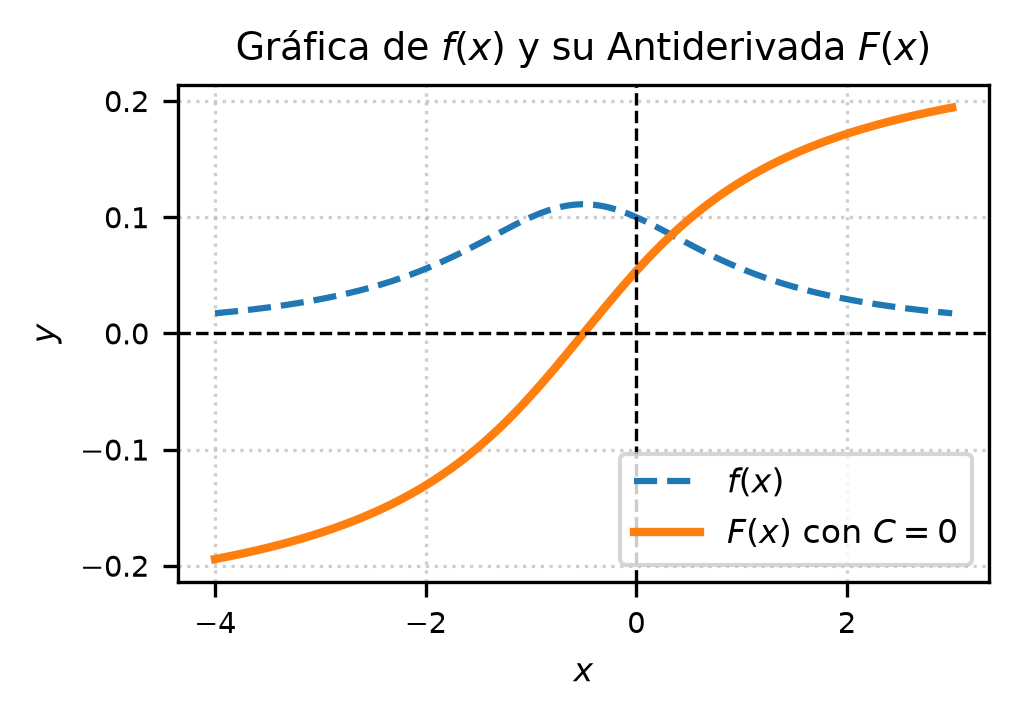
\includegraphics[width=\columnwidth]{semana_03/graficas/SEM03_P01_grafica.png}
	\caption{Representación gráfica de $f(x)$ y su antiderivada $F(x)$ evaluada para la constante de integración $C = 0$ (Problema 01).}
	\label{fig:problema01}
\end{figure}

	\subsection*{Problema 02}

\textbf{Enunciado:} Calcular la integral:
\begin{equation*}
\int \dfrac{(x-1)dx}{3x^2 - 4x + 3}
\end{equation*}

\textbf{Solución:} 
Primero, analizamos el denominador 
$D(x) = 3x^2 - 4x + 3$. 
Su discriminante es $\Delta = (-4)^2 - 4(3)(3) = 16 - 36 = -20 < 0$, 
por lo que es irreducible en los reales. La derivada 
del denominador es $D'(x) = 6x - 4$.

Modificamos el numerador para que contenga 
a $6x - 4$:
\begin{align*}
x - 1 &= \dfrac{1}{6}(6x - 6) \\
&= \dfrac{1}{6}(6x - 4 - 2)
\end{align*}

Sustituimos esto en la integral original:
\begin{align*}
I &= \int \dfrac{\frac{1}{6}(6x - 4 - 2)}{3x^2 - 4x + 3} dx \\
&= \dfrac{1}{6} \int \dfrac{6x - 4}{3x^2 - 4x + 3} dx \\
&\quad - \dfrac{2}{6} \int \dfrac{dx}{3x^2 - 4x + 3}
\end{align*}

La primera integral es inmediata por sustitución 
$u = 3x^2 - 4x + 3$:
\begin{equation*}
I_1 = \dfrac{1}{6} \ln|3x^2 - 4x + 3|
\end{equation*}

Para la segunda integral, completamos cuadrados 
en el denominador:
\begin{align*}
3x^2 - 4x + 3 &= 3\left(x^2 - \dfrac{4}{3}x + 1\right) \\
&= 3\left[\left(x - \dfrac{2}{3}\right)^2 + \dfrac{5}{9}\right]
\end{align*}

Sustituimos esto en la segunda integral:
\begin{align*}
I_2 &= -\dfrac{1}{3} \int \dfrac{dx}{3\left[\left(x - \dfrac{2}{3}\right)^2 + \dfrac{5}{9}\right]} \\
&= -\dfrac{1}{9} \int \dfrac{dx}{\left(x - \dfrac{2}{3}\right)^2 + \left(\dfrac{\sqrt{5}}{3}\right)^2}
\end{align*}

Aplicando la fórmula de la arcotangente:
\begin{align*}
I_2 &= -\dfrac{1}{9} \left(\dfrac{3}{\sqrt{5}}\right) 
\arctan\left(\dfrac{x - \frac{2}{3}}{\frac{\sqrt{5}}{3}}\right) \\
&= -\dfrac{1}{3\sqrt{5}} \arctan\left(\dfrac{3x - 2}{\sqrt{5}}\right)
\end{align*}

Combinando ambos resultados, la solución general 
es:
\begin{align*}
I &= \dfrac{1}{6} \ln(3x^2 - 4x + 3) \\
&\quad - \dfrac{\sqrt{5}}{15} \arctan\left(\dfrac{3x - 2}{\sqrt{5}}\right) + C
\end{align*}

\begin{figure}[H]
	\centering
	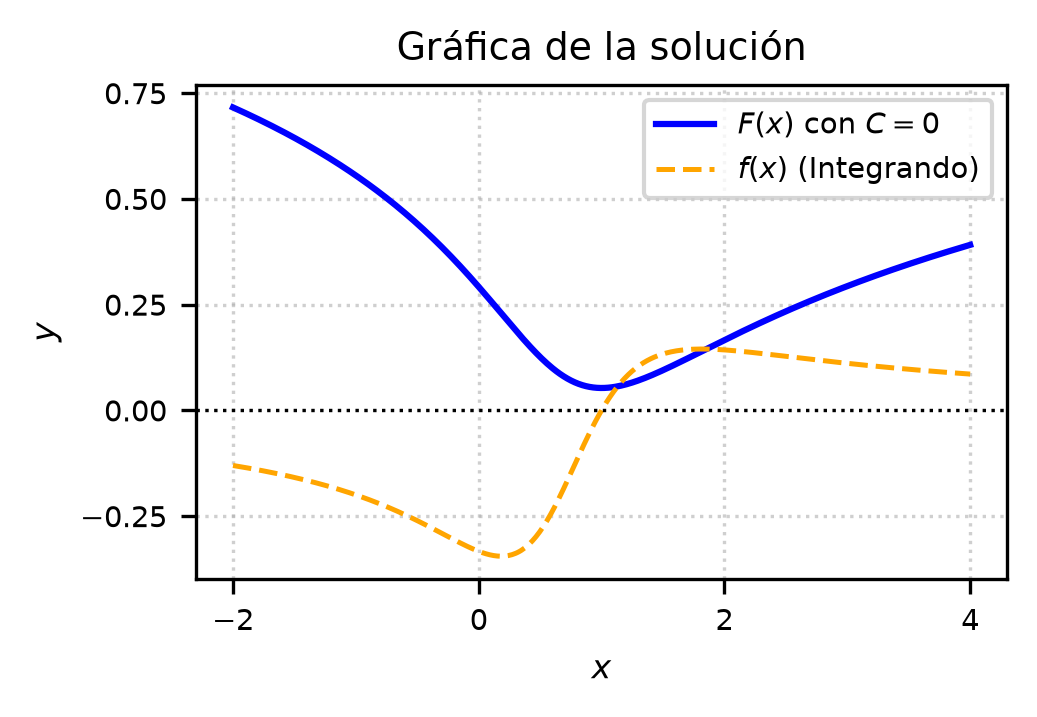
\includegraphics[width=\columnwidth]{semana_03/graficas/SEM03_P02_grafica.png}
	\caption{Representación gráfica de $f(x)$ y su antiderivada $F(x)$ evaluada para la constante de integración $C = 0$ (Problema 02).}
	\label{fig:problema02}
\end{figure}

	\subsection*{Problema 03}

\textbf{Enunciado:} Calcular la integral:
\begin{equation*}
\int \frac{(2x-3)dx}{x^2 + 6x + 15}
\end{equation*}

\textbf{Solución:} Para resolver esta integral racional, analizamos el denominador $x^2 + 6x + 15$. Su derivada es $2x + 6$. 

Siguiendo la indicación, reescribimos el numerador de manera que aparezca la derivada del denominador, ajustando con una constante:
\begin{equation*}
2x - 3 = (2x + 6) - 9
\end{equation*}

Sustituimos esta expresión en la integral original y la separamos en dos integrales distintas:
\begin{align*}
I &= \int \frac{2x - 3}{x^2 + 6x + 15} \, dx \\
&= \int \frac{2x + 6}{x^2 + 6x + 15} \, dx \\
&\quad - \int \frac{9}{x^2 + 6x + 15} \, dx
\end{align*}

Para la primera integral, hacemos el cambio de variable $u = x^2 + 6x + 15$, cuyo diferencial es $du = (2x + 6)dx$:
\begin{align*}
I_1 &= \int \frac{2x + 6}{x^2 + 6x + 15} \, dx \\
&= \ln|x^2 + 6x + 15|
\end{align*}

Para la segunda integral, completamos el trinomio cuadrado perfecto en el denominador:
\begin{align*}
x^2 + 6x + 15 &= (x^2 + 6x + 9) - 9 + 15 \\
&= (x + 3)^2 + 6
\end{align*}

Reescribimos la segunda integral en función de esta forma estándar de arco tangente:
\begin{align*}
I_2 &= 9 \int \frac{dx}{(x + 3)^2 + 6} \\
&= \frac{9}{\sqrt{6}} \arctan\left(\frac{x + 3}{\sqrt{6}}\right)
\end{align*}

Combinando ambos resultados y añadiendo la constante de integración $C$, obtenemos la solución general:
\begin{align*}
I &= \ln(x^2 + 6x + 15) \\
&\quad - \frac{3\sqrt{6}}{2} \arctan\left(\frac{x + 3}{\sqrt{6}}\right) + C
\end{align*}

\begin{figure}[H]
	\centering
	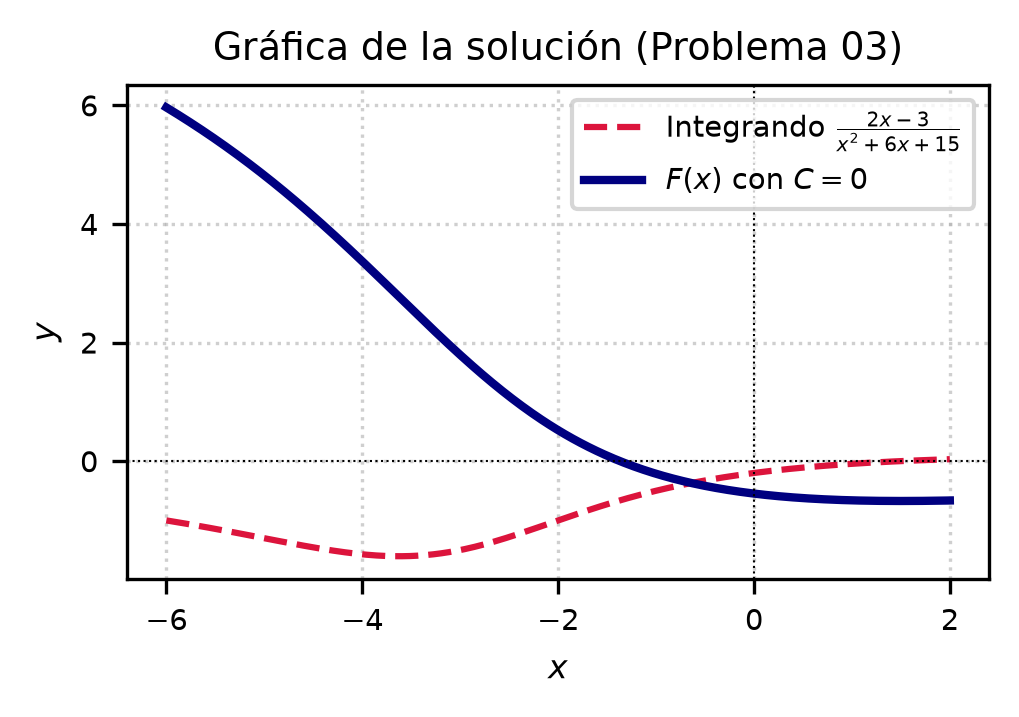
\includegraphics[width=\columnwidth]{semana_03/graficas/SEM03_P03_grafica.png}
	\caption{Representación gráfica de $f(x)$ y su antiderivada $F(x)$ evaluada para la constante de integración $C = 0$ (Problema 03).}
	\label{fig:problema03}
\end{figure}

	\subsection*{Problema 04}

\textbf{Enunciado:} Calcular la integral:\\
$\int \dfrac{2x+2}{x^2 - 4x + 9} \, dx$

\textbf{Solución:} \
Siguiendo las indicaciones, buscamos que el numerador contenga la derivada del denominador, la cual es $D_x(x^2 - 4x + 9) = 2x - 4$. 

Manipulamos algebraicamente el numerador sumando y restando $4$:
\begin{align*}
2x + 2 &= 2x - 4 + 4 + 2 \\
&= (2x - 4) + 6
\end{align*}

Sustituimos esta expresión en la integral original y la separamos en dos partes:
\begin{align*}
I &= \int \dfrac{(2x - 4) + 6}{x^2 - 4x + 9} \, dx \\
&= \int \dfrac{2x - 4}{x^2 - 4x + 9} \, dx \\
&\quad + \int \dfrac{6}{x^2 - 4x + 9} \, dx
\end{align*}

Para la primera integral ($I_1$), aplicamos el método de sustitución haciendo $u = x^2 - 4x + 9$, de donde $du = (2x - 4) \, dx$:
\begin{align*}
I_1 &= \int \dfrac{du}{u} = \ln|u| \\
&= \ln|x^2 - 4x + 9|
\end{align*}

Para la segunda integral ($I_2$), completamos el trinomio cuadrado en el denominador:
\begin{align*}
x^2 - 4x + 9 &= (x^2 - 4x + 4) - 4 + 9 \\
&= (x - 2)^2 + 5
\end{align*}

Sustituimos $I_2$ utilizando la fórmula de integración $\int \dfrac{1}{u^2 + a^2} \, du = \dfrac{1}{a}\arctan\left(\dfrac{u}{a}\right)$:
\begin{align*}
I_2 &= \int \dfrac{6}{(x-2)^2 + 5} \, dx \\
&= \dfrac{6}{\sqrt{5}} \arctan\left(\dfrac{x - 2}{\sqrt{5}}\right)
\end{align*}

Finalmente, unimos ambas soluciones y añadimos la constante de integración $C$:
\begin{align*}
I &= \ln(x^2 - 4x + 9) \\
&\quad + \dfrac{6}{\sqrt{5}} \arctan\left(\dfrac{x - 2}{\sqrt{5}}\right) + C
\end{align*}

\begin{figure}[H]
	\centering
	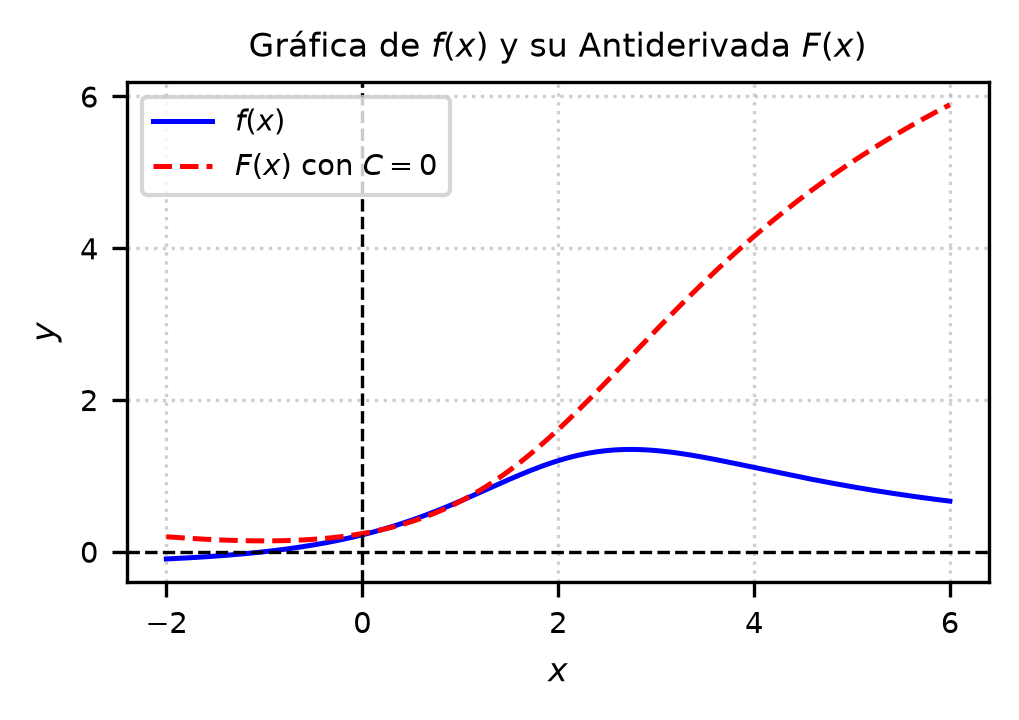
\includegraphics[width=\columnwidth]{semana_03/graficas/SEM03_P04_grafica.png}
	\caption{Representación gráfica de $f(x)$ y su antiderivada $F(x)$ evaluada para la constante de integración $C = 0$ (Problema 04).}
	\label{fig:problema04}
\end{figure}

	\subsection*{Problema 05}

\textbf{Enunciado:} \\
Calcular la siguiente integral indefinida:
\begin{align*}
\int \dfrac{2x - 3}{x^2 + 6x + 15} \, dx
\end{align*}

\textbf{Solución:} \\
Para resolver esta integral, buscamos en el numerador la derivada del denominador. 
El denominador es $u = x^2 + 6x + 15$, cuya derivada es $u' = 2x + 6$.

Manipulamos algebraicamente el numerador para que aparezca dicha derivada:
\begin{align*}
2x - 3 &= (2x + 6) - 6 - 3 \\
&= (2x + 6) - 9
\end{align*}

Sustituimos esto en la integral original y separamos en dos integrales:
\begin{align*}
&\int \dfrac{2x - 3}{x^2 + 6x + 15} \, dx = \\
&\int \dfrac{2x + 6}{x^2 + 6x + 15} \, dx - 9 \int \dfrac{1}{x^2 + 6x + 15} \, dx
\end{align*}

Resolvemos la primera integral usando sustitución $u = x^2 + 6x + 15$, $du = (2x + 6) \, dx$:
\begin{align*}
\int \dfrac{2x + 6}{x^2 + 6x + 15} \, dx &= \ln|x^2 + 6x + 15|
\end{align*}

Para la segunda integral, completamos el trinomio cuadrado perfecto en el denominador:
\begin{align*}
x^2 + 6x + 15 &= (x^2 + 6x + 9) + 6 \\
&= (x + 3)^2 + (\sqrt{6})^2
\end{align*}

Aplicamos la fórmula de integración para la arcotangente:
\begin{align*}
&\int \dfrac{1}{(x + 3)^2 + (\sqrt{6})^2} \, dx \\
&= \dfrac{1}{\sqrt{6}} \arctan\left(\dfrac{x + 3}{\sqrt{6}}\right)
\end{align*}

Combinando ambos resultados y añadiendo la constante de integración $C$, obtenemos la solución final:
\begin{align*}
\int &\dfrac{2x - 3}{x^2 + 6x + 15} \, dx = \\
&\ln|x^2 + 6x + 15| \\
&- \dfrac{9}{\sqrt{6}} \arctan\left(\dfrac{x + 3}{\sqrt{6}}\right) + C
\end{align*}

\begin{figure}[H]
	\centering
	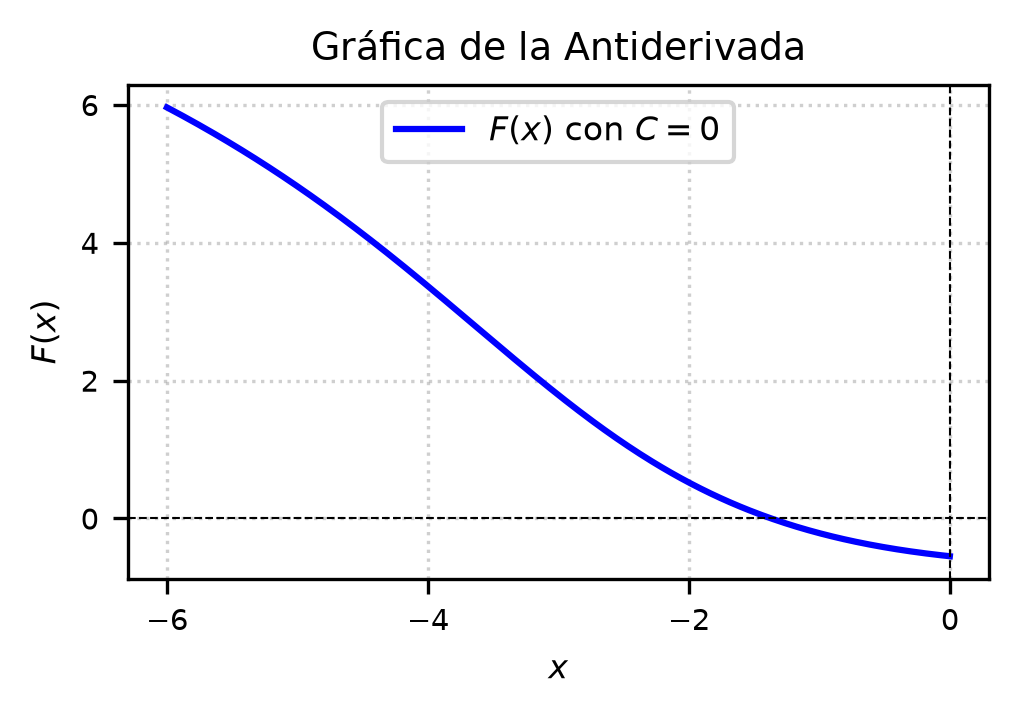
\includegraphics[width=\columnwidth]{semana_03/graficas/SEM03_P05_grafica.png}
	\caption{Representación gráfica de $f(x)$ y su antiderivada $F(x)$ evaluada para la constante de integración $C = 0$ (Problema 05).}
	\label{fig:problema05}
\end{figure}

	\subsection*{Problema 06}
\textbf{Enunciado:} Calcular la integral:
\begin{equation*}
\int \dfrac{x + 2}{x^2 + 2x + 2} \, dx
\end{equation*}

\textbf{Solución:}
Para resolver la integral dada, analizamos primero el denominador. Derivando la expresión cuadrática $x^2 + 2x + 2$, obtenemos $2x + 2$. 

Buscamos que el numerador contenga la derivada del denominador. Para ello, reescribimos el numerador $(x + 2)$ utilizando la sugerencia dada:
\begin{align*}
x + 2 &= (x + 1) + 1 \\
&= \dfrac{1}{2}(2x + 2) + 1
\end{align*}

Sustituimos esta nueva forma del numerador en la integral original:
\begin{align*}
\int &\dfrac{x + 2}{x^2 + 2x + 2} \, dx = \\
&\int \dfrac{\frac{1}{2}(2x + 2) + 1}{x^2 + 2x + 2} \, dx
\end{align*}

Separamos la integral en dos partes para facilitar su integración:
\begin{align*}
&= \dfrac{1}{2} \int \dfrac{2x + 2}{x^2 + 2x + 2} \, dx \\
&\quad + \int \dfrac{1}{x^2 + 2x + 2} \, dx
\end{align*}

Para la primera integral, aplicamos sustitución simple con $u = x^2 + 2x + 2$ y $du = (2x + 2) \, dx$. Para la segunda, completamos el trinomio cuadrado perfecto en el denominador: $x^2 + 2x + 2 = (x + 1)^2 + 1$.

\begin{align*}
&= \dfrac{1}{2} \int \dfrac{du}{u} + \int \dfrac{1}{(x+1)^2 + 1} \, dx
\end{align*}

Resolvemos ambas integrales estándar:
\begin{align*}
&= \dfrac{1}{2} \ln|x^2 + 2x + 2| \\
&\quad + \arctan(x + 1) + C
\end{align*}

Dado que $x^2 + 2x + 2 > 0$ para todo número real $x$, podemos prescindir del valor absoluto. La solución general es:
\begin{align*}
F(x) &= \dfrac{1}{2} \ln(x^2 + 2x + 2) \\
&\quad + \arctan(x + 1) + C
\end{align*}

\begin{figure}[H]
	\centering
	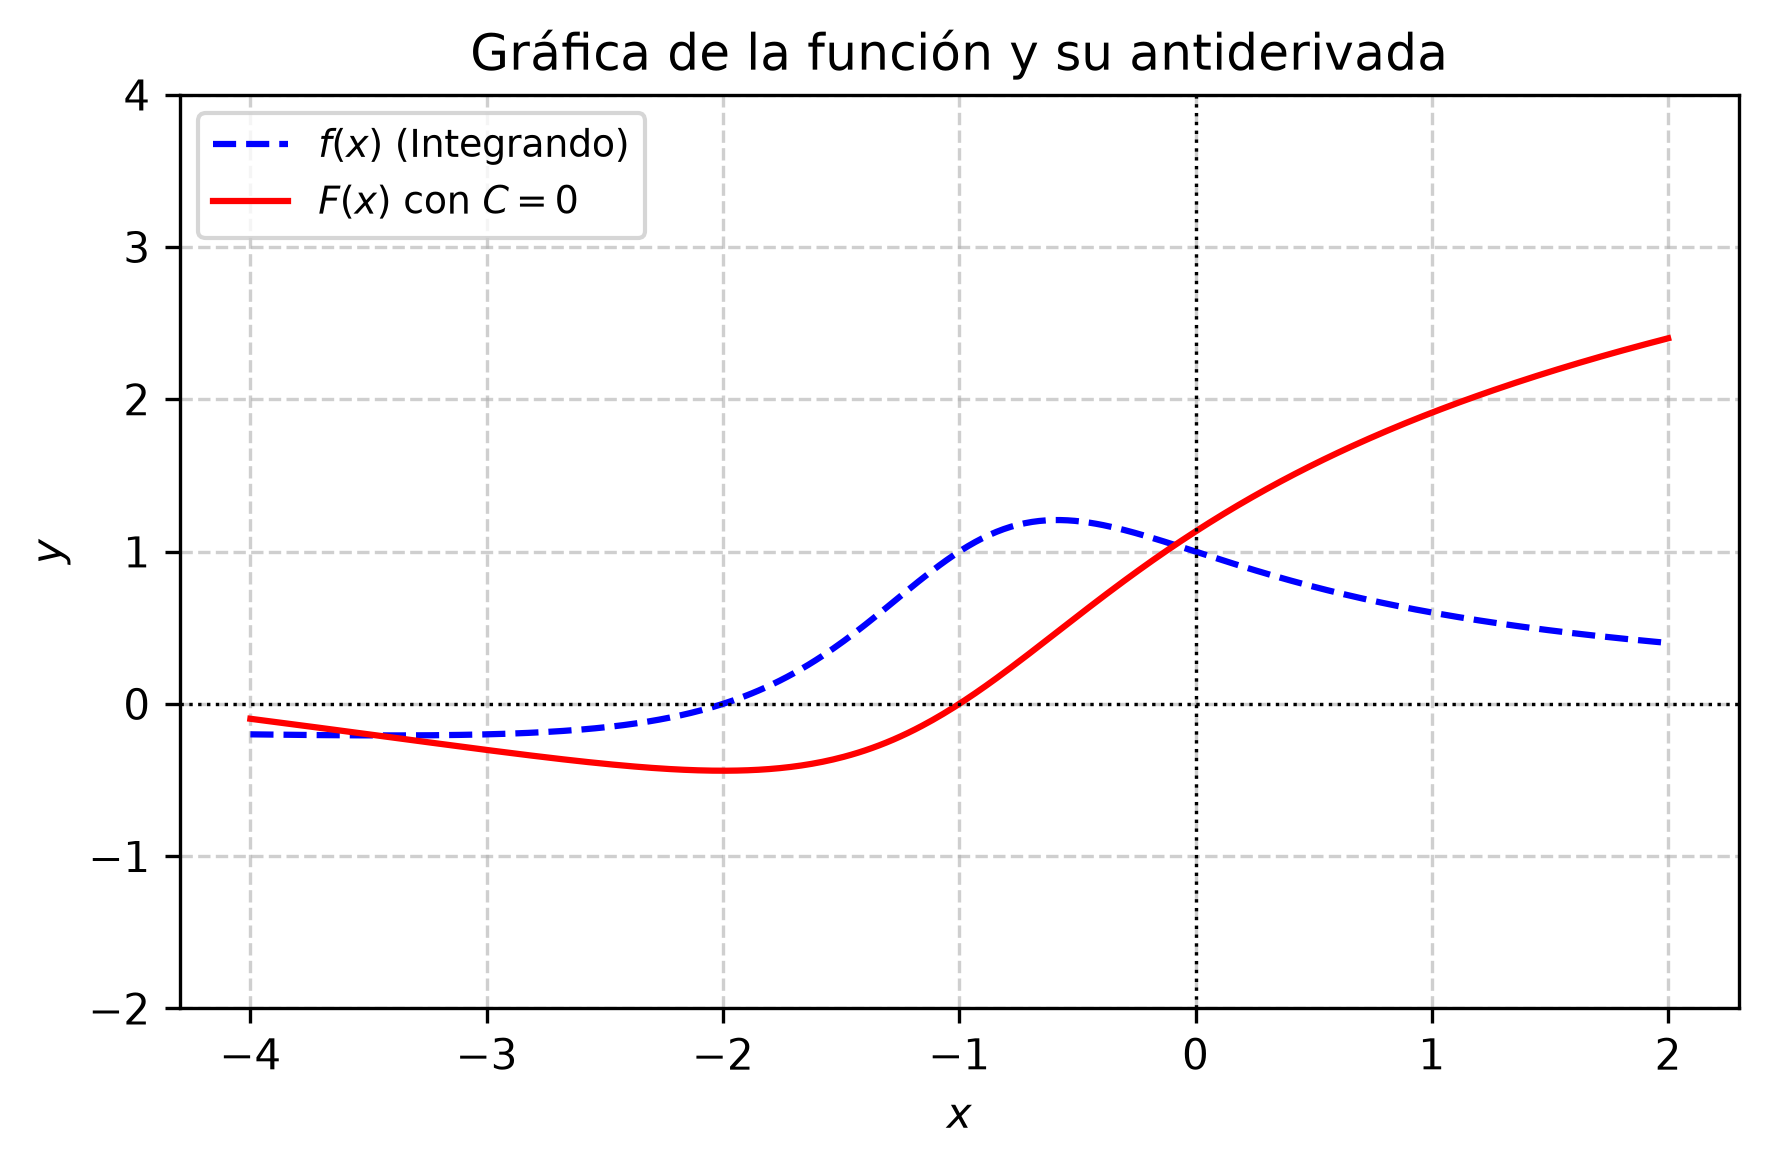
\includegraphics[width=\columnwidth]{semana_03/graficas/SEM03_P06_grafica.png}
	\caption{Representación gráfica de $f(x)$ y su antiderivada $F(x)$ evaluada para la constante de integración $C = 0$ (Problema 06).}
	\label{fig:problema06}
\end{figure}

	\subsection*{Problema 07}

\textbf{Enunciado:} 
Calcular la integral indefinida:
\begin{align*}
I = \int \dfrac{x \, dx}{x^2 - 4x + 4}
\end{align*}

\textbf{Solución:} 
Primero, analizamos el denominador de la función integrandia. Notamos que el trinomio cuadrado perfecto se puede factorizar de la siguiente manera:
\begin{align*}
x^2 - 4x + 4 = (x - 2)^2
\end{align*}

Sustituyendo esto en la integral dada, la expresión se reescribe como:
\begin{align*}
I = \int \dfrac{x}{(x - 2)^2} \, dx
\end{align*}

Para resolver esta integral, podemos utilizar el método de sustitución algebraica. Definimos una nueva variable $u$ tal que:
\begin{align*}
u &= x - 2 \\
du &= dx
\end{align*}

Además, despejamos la variable $x$ de la sustitución para expresarla en términos de $u$:
\begin{align*}
x = u + 2
\end{align*}

Sustituyendo $u$, $du$ y $x$ en la integral original, obtenemos:
\begin{align*}
I &= \int \dfrac{u + 2}{u^2} \, du
\end{align*}

Separamos la fracción en dos términos distintos para facilitar la integración:
\begin{align*}
I &= \int \left( \dfrac{u}{u^2} + \dfrac{2}{u^2} \right) du \\
I &= \int \left( \dfrac{1}{u} + 2u^{-2} \right) du
\end{align*}

Integramos cada término por separado aplicando las reglas básicas de integración:
\begin{align*}
I &= \int \dfrac{1}{u} \, du + \int 2u^{-2} \, du \\
I &= \ln|u| + 2 \left( \dfrac{u^{-1}}{-1} \right) + C \\
I &= \ln|u| - \dfrac{2}{u} + C
\end{align*}

Finalmente, regresamos a la variable original $x$ sustituyendo $u = x - 2$:
\begin{align*}
I = \ln|x - 2| - \dfrac{2}{x - 2} + C
\end{align*}

\begin{figure}[H]
	\centering
	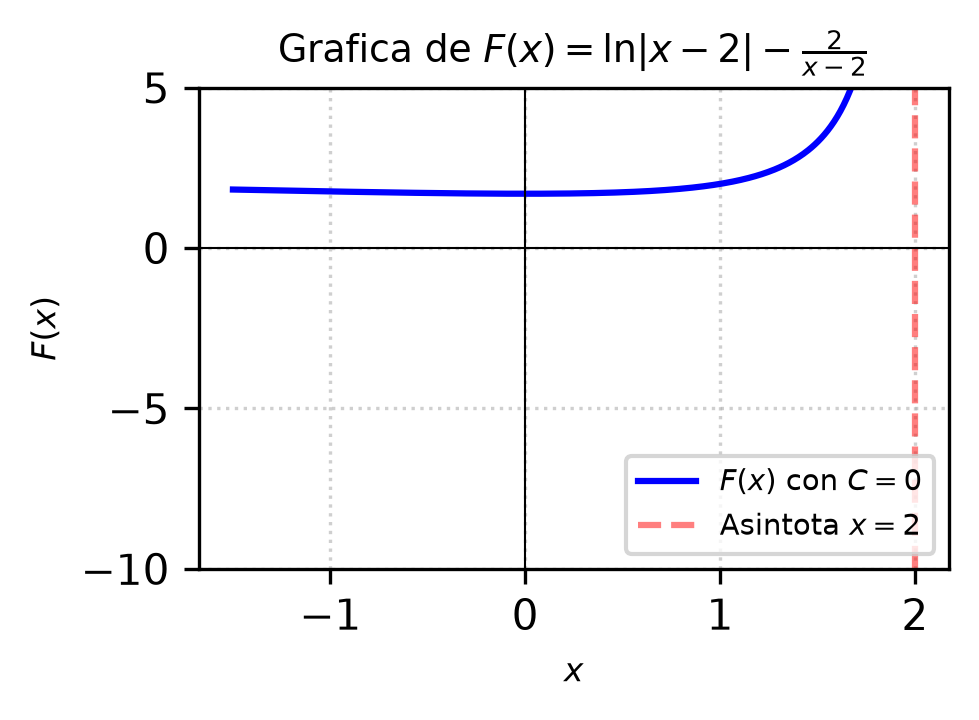
\includegraphics[width=\columnwidth]{semana_03/graficas/SEM03_P07_grafica.png}
	\caption{Representación gráfica de $f(x)$ y su antiderivada $F(x)$ evaluada para la constante de integración $C = 0$ (Problema 07).}
	\label{fig:problema07}
\end{figure}

	\subsection*{Problema 08}

\textbf{Enunciado:} \\
Calcular la integral indefinida:
\begin{align*}
\int \dfrac{2x^2 + 3}{x^3 - 2x^2 + x} \, dx
\end{align*}

\textbf{Solución:} \\
Primero, factorizamos el denominador de la función racional:
\begin{align*}
x^3 - 2x^2 + x &= x(x^2 - 2x + 1) \\
&= x(x - 1)^2
\end{align*}

Planteamos la descomposición en fracciones parciales sugerida:
\begin{align*}
\dfrac{2x^2 + 3}{x(x - 1)^2} = \dfrac{A}{x} + \dfrac{B}{x - 1} + \dfrac{C}{(x - 1)^2}
\end{align*}

Multiplicamos toda la ecuación por el denominador común $x(x - 1)^2$:
\begin{align*}
2x^2 + 3 &= A(x - 1)^2 \\
&\quad + Bx(x - 1) + Cx
\end{align*}

Para hallar los valores de las constantes, evaluamos en valores convenientes de $x$:

Si $x = 0$:
\begin{align*}
2(0)^2 + 3 &= A(0 - 1)^2 + 0 + 0 \\
3 &= A(1) \implies A = 3
\end{align*}

Si $x = 1$:
\begin{align*}
2(1)^2 + 3 &= 0 + 0 + C(1) \\
5 &= C \implies C = 5
\end{align*}

Para hallar $B$, usamos $x = 2$ y el valor de $A = 3$, $C = 5$:
\begin{align*}
2(2)^2 + 3 &= 3(2 - 1)^2 \\
&\quad + B(2)(2 - 1) + 5(2) \\
11 &= 3(1) + 2B + 10 \\
11 &= 13 + 2B \implies 2B = -2 \\
B &= -1
\end{align*}

Sustituimos las constantes $A$, $B$ y $C$ en la integral:
\begin{align*}
\int &\left( \dfrac{3}{x} - \dfrac{1}{x - 1} + \dfrac{5}{(x - 1)^2} \right) dx
\end{align*}

integramos término a término:
\begin{align*}
&= 3\ln|x| - \ln|x - 1| \\
&\quad - \dfrac{5}{x - 1} + K
\end{align*}

Por lo tanto, la solución general es:
\begin{align*}
\int &\dfrac{2x^2 + 3}{x^3 - 2x^2 + x} \, dx \\
&= \ln\left|\dfrac{x^3}{x - 1}\right| - \dfrac{5}{x - 1} + K
\end{align*}

\begin{figure}[H]
	\centering
	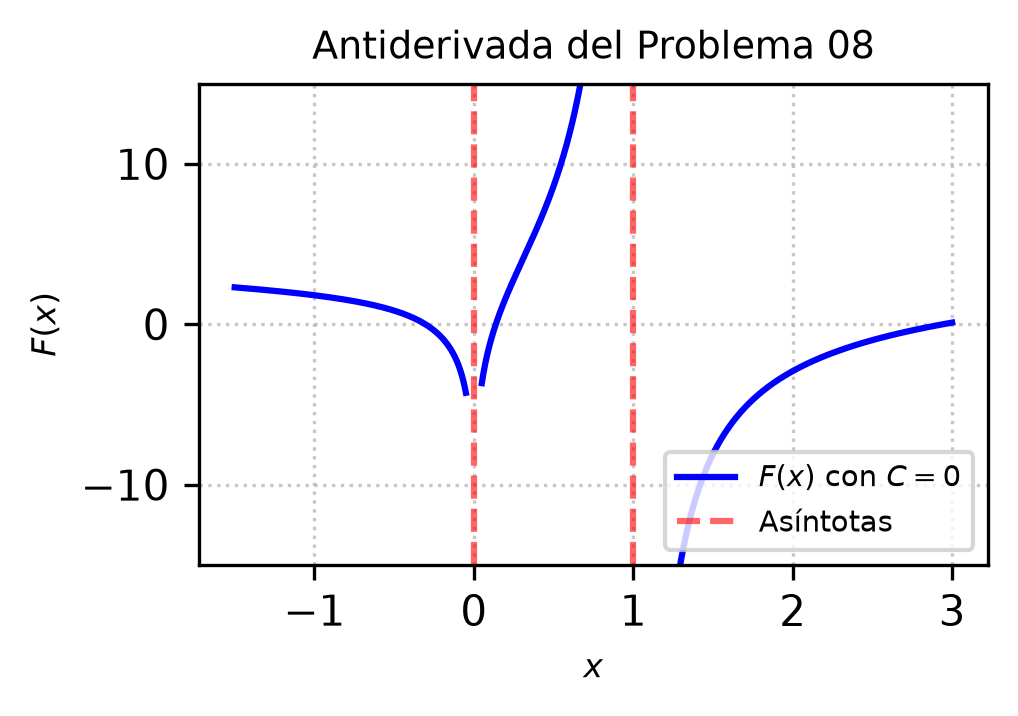
\includegraphics[width=\columnwidth]{semana_03/graficas/SEM03_P08_grafica.png}
	\caption{Representación gráfica de $f(x)$ y su antiderivada $F(x)$ evaluada para la constante de integración $C = 0$ (Problema 08).}
	\label{fig:problema08}
\end{figure}

	\subsection*{Problema 09}

\noindent\textbf{Enunciado:} Calcular la integral:
\begin{equation*}
\int \dfrac{x^4 - 6x^3 + 12x^2 + 6}{x^3 - 6x^2 + 12x - 8} \, dx
\end{equation*}

\noindent\textbf{Solución:} Primero, observamos que el denominador es el binomio al cubo expandido:
\begin{equation*}
x^3 - 6x^2 + 12x - 8 = (x - 2)^3
\end{equation*}

Dado que el grado del numerador es mayor que el del denominador, realizamos la división polinómica de $x^4 - 6x^3 + 12x^2 + 6$ entre $x^3 - 6x^2 + 12x - 8$. Al dividir, obtenemos un cociente de $x$ y un residuo de $6$. Es decir:
\begin{equation*}
\dfrac{x^4 - 6x^3 + 12x^2 + 6}{(x - 2)^3} = x + \dfrac{6}{(x - 2)^3}
\end{equation*}

Reescribimos la integral original utilizando esta descomposición:
\begin{equation*}
\int \left( x + \dfrac{6}{(x - 2)^3} \right) dx
\end{equation*}

Separamos la integral en dos términos más sencillos:
\begin{equation*}
= \int x \, dx + \int \dfrac{6}{(x - 2)^3} \, dx
\end{equation*}

La primera integral es inmediata:
\begin{equation*}
\int x \, dx = \dfrac{x^2}{2}
\end{equation*}

Para la segunda integral, aplicamos sustitución simple haciendo $u = x - 2$, de modo que $du = dx$:
\begin{align*}
\int \dfrac{6}{(x - 2)^3} \, dx &= 6 \int u^{-3} \, du \\
&= 6 \left( \dfrac{u^{-2}}{-2} \right) \\
&= -\dfrac{3}{u^2}
\end{align*}

Regresando a la variable original $x$:
\begin{equation*}
-\dfrac{3}{u^2} = -\dfrac{3}{(x - 2)^2}
\end{equation*}

Finalmente, combinamos ambos resultados y añadimos la constante de integración $C$:
\begin{equation*}
\dfrac{x^2}{2} - \dfrac{3}{(x - 2)^2} + C
\end{equation*}

\begin{figure}[H]
	\centering
	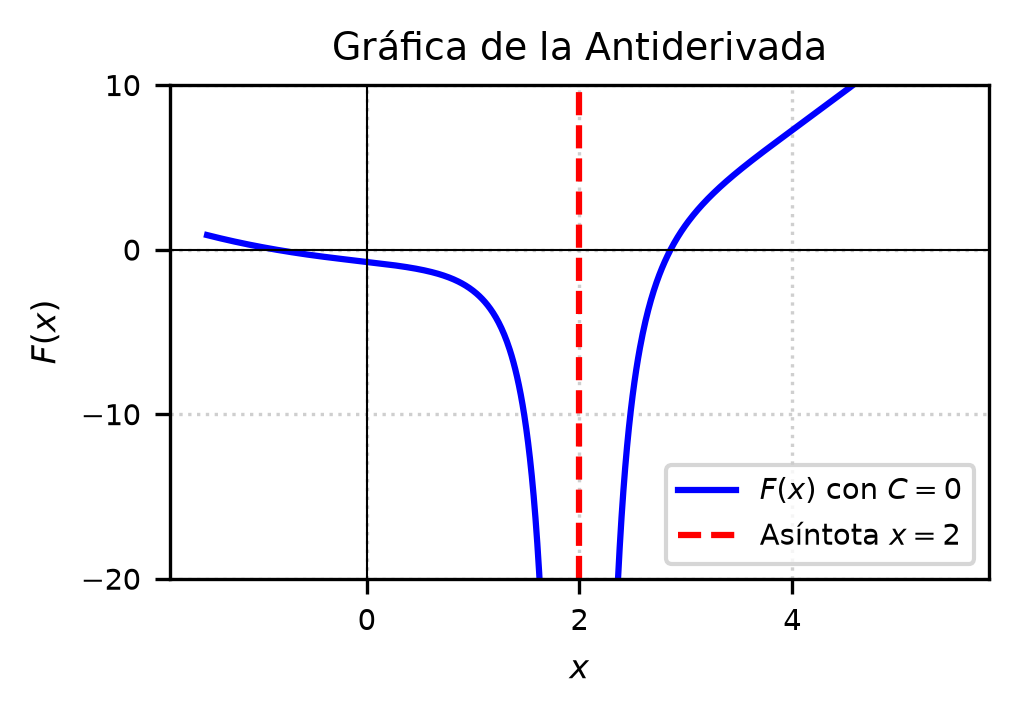
\includegraphics[width=\columnwidth]{semana_03/graficas/SEM03_P09_grafica.png}
	\caption{Representación gráfica de $f(x)$ y su antiderivada $F(x)$ evaluada para la constante de integración $C = 0$ (Problema 09).}
	\label{fig:problema09}
\end{figure}

	\subsection*{Problema 10}

\textbf{Enunciado:} Calcular la integral:
\begin{align*}
\int \dfrac{x^3 + x^2 + x + 3}{x^4 + 4x^2 + 3} \, dx
\end{align*}

\textbf{Solución:} El denominador se puede factorizar como indica la sugerencia:
\begin{align*}
x^4 + 4x^2 + 3 = (x^2 + 1)(x^2 + 3)
\end{align*}

Planteamos la descomposición en fracciones parciales:
\begin{align*}
\dfrac{x^3 + x^2 + x + 3}{(x^2 + 1)(x^2 + 3)} &= \dfrac{Ax + B}{x^2 + 1} \\
&+ \dfrac{Cx + D}{x^2 + 3}
\end{align*}

Multiplicando por el denominador común, obtenemos:
\begin{align*}
x^3 + &x^2 + x + 3 = (Ax + B)(x^2 + 3) \\
&+ (Cx + D)(x^2 + 1)
\end{align*}

Expandiendo y agrupando términos según las potencias de $x$:
\begin{align*}
x^3 + x^2 + x + 3 &= (A + C)x^3 \\
&+ (B + D)x^2 \\
&+ (3A + C)x + (3B + D)
\end{align*}

Igualando los coeficientes de ambos lados de la ecuación, formamos el sistema:
\begin{align*}
A + C &= 1 \\
B + D &= 1 \\
3A + C &= 1 \\
3B + D &= 3
\end{align*}

Resolviendo el sistema para las variables:
\begin{align*}
\text{De } 3A + C &= 1 \text{ y } A + C = 1: \\
2A &= 0 \implies A = 0, \ C = 1 \\
\text{De } 3B + D &= 3 \text{ y } B + D = 1: \\
2B &= 2 \implies B = 1, \ D = 0
\end{align*}

Sustituyendo los valores hallados en las fracciones parciales:
\begin{align*}
\int \dfrac{1}{x^2 + 1} \, dx + \int \dfrac{x}{x^2 + 3} \, dx
\end{align*}

Calculando cada integral por separado, la primera es inmediata y la segunda requiere una sustitución $u = x^2 + 3$:
\begin{align*}
\int \dfrac{1}{x^2 + 1} \, dx &= \arctan(x) \\
\int \dfrac{x}{x^2 + 3} \, dx &= \dfrac{1}{2} \ln|x^2 + 3|
\end{align*}

Combinando los resultados y añadiendo la constante de integración $C$:
\begin{align*}
\int \dfrac{x^3 + x^2 + x + 3}{x^4 + 4x^2 + 3} \, dx = \\
\arctan(x) + \dfrac{1}{2} \ln(x^2 + 3) + C
\end{align*}

\begin{figure}[H]
	\centering
	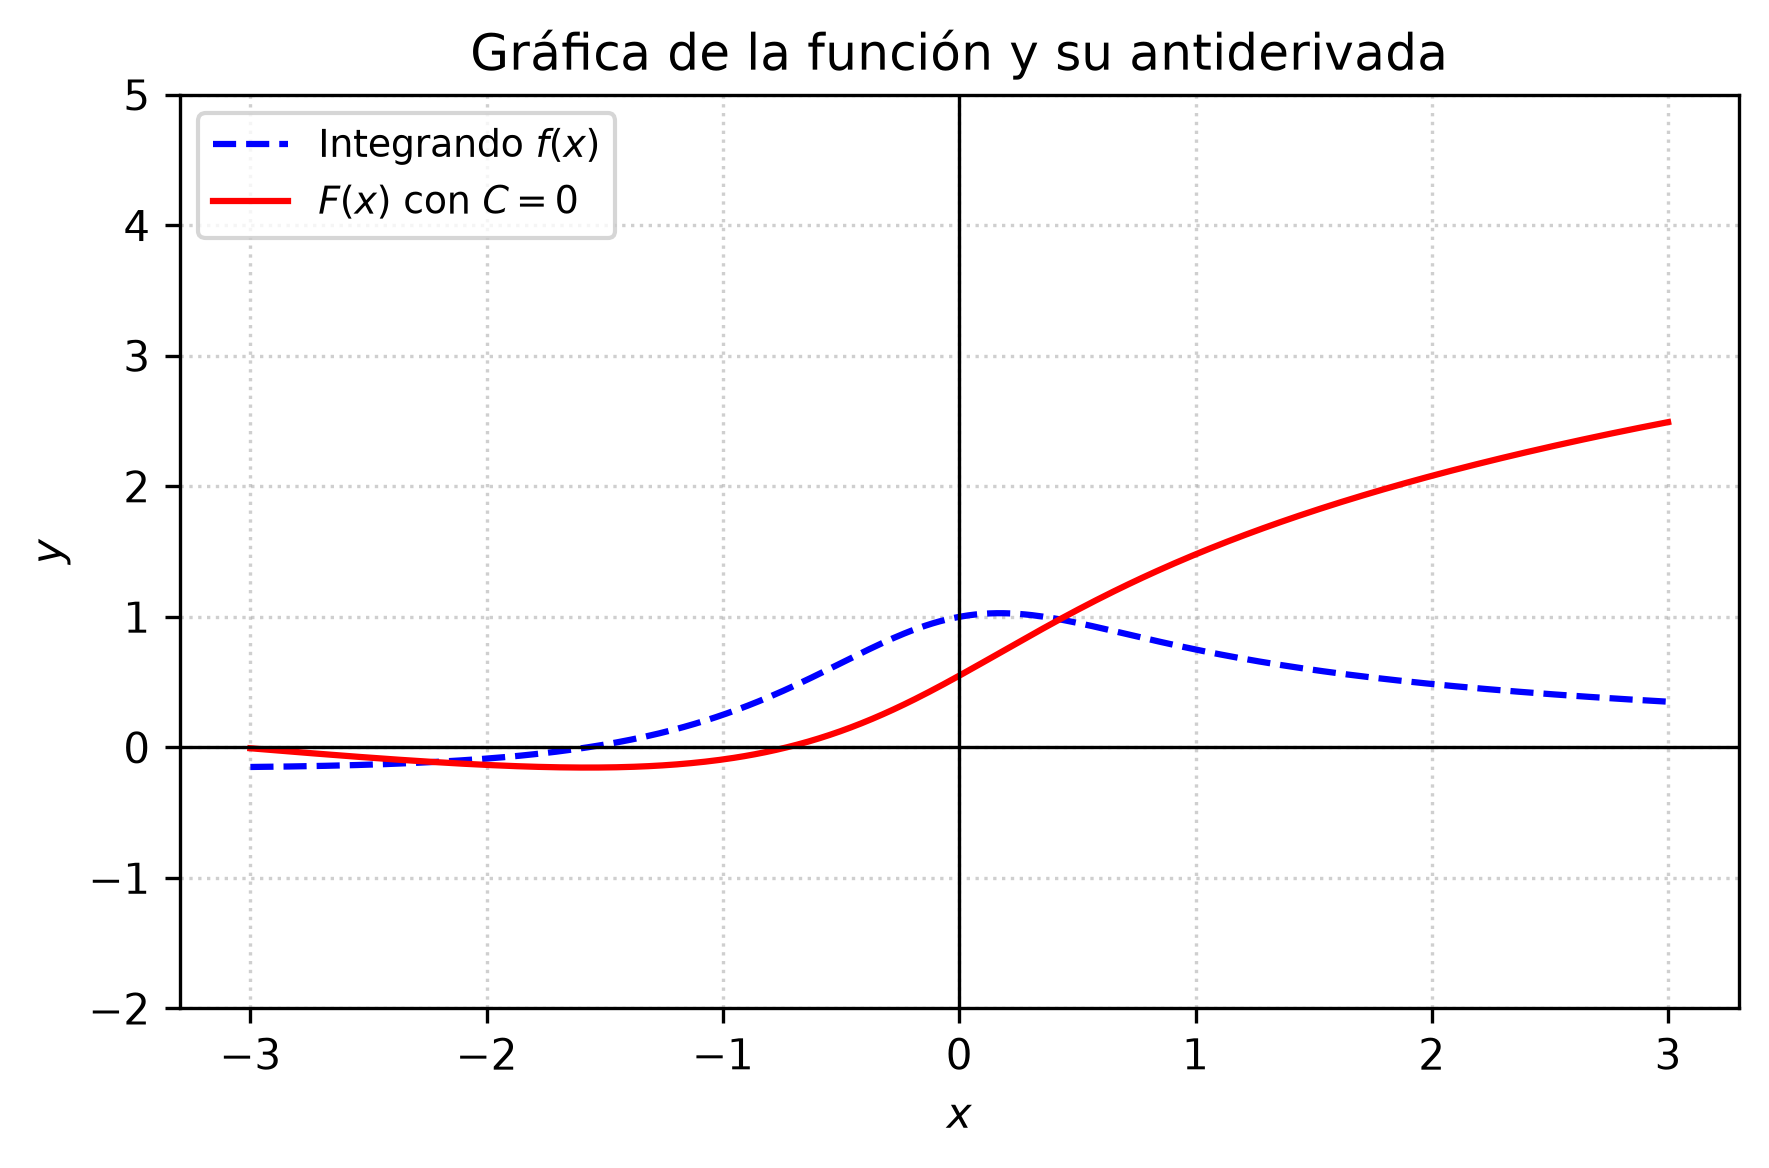
\includegraphics[width=\columnwidth]{semana_03/graficas/SEM03_P10_grafica.png}
	\caption{Representación gráfica de $f(x)$ y su antiderivada $F(x)$ evaluada para la constante de integración $C = 0$ (Problema 10).}
	\label{fig:problema10}
\end{figure}

	\subsection*{Problema 11}

\noindent\textbf{Enunciado:} \\
Calcular la integral indefinida:
\begin{align*}
\int \frac{x^4}{x^4 + 2x^2 + 1} \, dx
\end{align*}

\noindent\textbf{Solución:} \\
Primero, notemos que el denominador es un trinomio cuadrado perfecto. Podemos reescribirlo como:
\begin{align*}
x^4 + 2x^2 + 1 = (x^2 + 1)^2
\end{align*}

Sustituyendo esto en la integral, la expresión se convierte en:
\begin{align*}
\int \frac{x^4}{(x^2 + 1)^2} \, dx
\end{align*}

Siguiendo la sugerencia de expresar el numerador de forma conveniente, reescribimos $x^4$ como:
\begin{align*}
x^4 &= (x^2 + 1)^2 - 2(x^2 + 1) + 1
\end{align*}

Sustituyendo este resultado en el integrando, dividimos término a término:
\begin{align*}
\frac{x^4}{(x^2+1)^2} &= \frac{(x^2+1)^2}{(x^2+1)^2} \\
&\quad - \frac{2(x^2+1)}{(x^2+1)^2} + \frac{1}{(x^2+1)^2}
\end{align*}

Simplificando cada término algebraicamente, obtenemos:
\begin{align*}
&= 1 - \frac{2}{x^2+1} + \frac{1}{(x^2+1)^2}
\end{align*}

Ahora, integramos cada parte por separado:
\begin{align*}
\int 1 \, dx &= x \\
\int \frac{-2}{x^2+1} \, dx &= -2 \arctan(x)
\end{align*}

Para la última integral, $\int \frac{1}{(x^2+1)^2} \, dx$, utilizamos la sustitución trigonométrica $x = \tan(\theta)$, de donde $dx = \sec^2(\theta) \, d\theta$:
\begin{align*}
\int \frac{\sec^2(\theta)}{(\tan^2(\theta)+1)^2} \, d\theta &= \int \frac{\sec^2(\theta)}{(\sec^2(\theta))^2} \, d\theta \\
&= \int \frac{1}{\sec^2(\theta)} \, d\theta \\
&= \int \cos^2(\theta) \, d\theta
\end{align*}

Usando la identidad del ángulo doble:
\begin{align*}
\int \frac{1 + \cos(2\theta)}{2} \, d\theta &= \frac{\theta}{2} + \frac{\sin(2\theta)}{4} \\
&= \frac{\theta}{2} + \frac{\sin(\theta)\cos(\theta)}{2}
\end{align*}

Volviendo a la variable original $x$:
\begin{align*}
&= \frac{\arctan(x)}{2} + \frac{x}{2(x^2+1)}
\end{align*}

Sumando todas las partes y agregando la constante de integración $C$, obtenemos la solución final:
\begin{align*}
\int \frac{x^4}{x^4 + 2x^2 + 1} \, dx &= x - 2\arctan(x) \\
&\quad + \frac{\arctan(x)}{2} \\
&\quad + \frac{x}{2(x^2+1)} + C
\end{align*}

Agrupando los términos semejantes de $\arctan(x)$:
\begin{align*}
&= x - \frac{3}{2}\arctan(x) \\
&\quad + \frac{x}{2(x^2+1)} + C
\end{align*}

\begin{figure}[H]
	\centering
	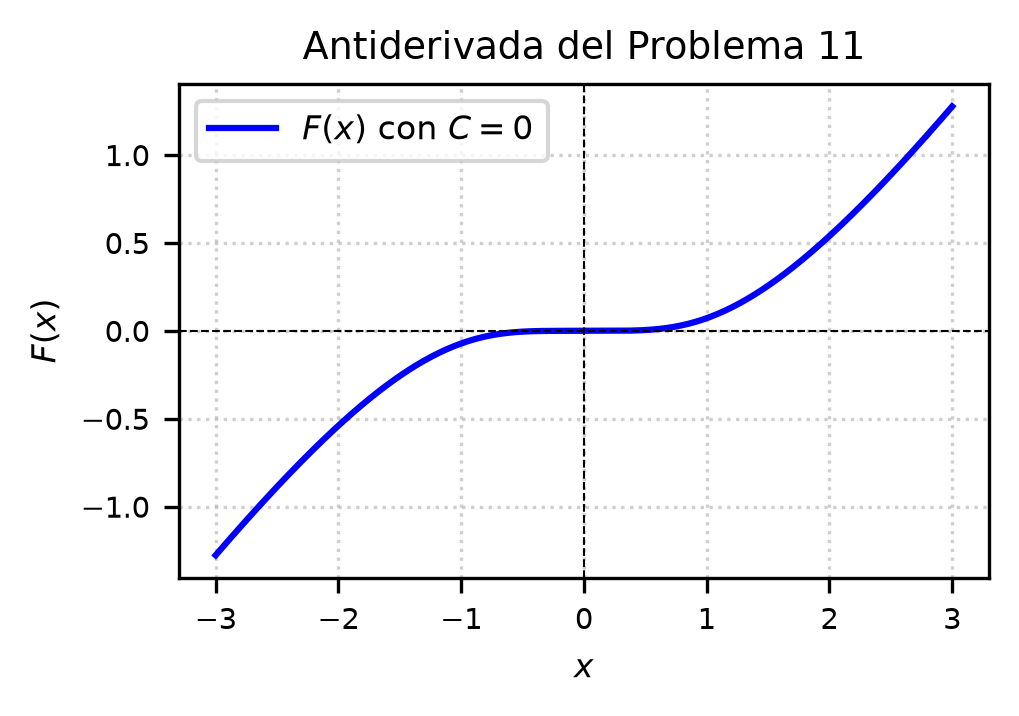
\includegraphics[width=\columnwidth]{semana_03/graficas/SEM03_P11_grafica.png}
	\caption{Representación gráfica de $f(x)$ y su antiderivada $F(x)$ evaluada para la constante de integración $C = 0$ (Problema 11).}
	\label{fig:problema11}
\end{figure}

	\subsection*{Problema 12}

\textbf{Enunciado:} 
Calcular la integral:
\begin{align*}
\int \dfrac{x^4}{x^4 - 1} \, dx
\end{align*}

\textbf{Solución:} 
Dado que el grado del numerador es igual al grado del denominador, realizamos la división polinómica:
\begin{align*}
\dfrac{x^4}{x^4 - 1} = 1 + \dfrac{1}{x^4 - 1}
\end{align*}

Factorizamos el denominador como se indica en las observaciones:
\begin{align*}
x^4 - 1 = (x - 1)(x + 1)(x^2 + 1)
\end{align*}

Planteamos la descomposición en fracciones parciales para la fracción restante:
\begin{align*}
\dfrac{1}{x^4 - 1} &= \dfrac{A}{x - 1} + \dfrac{B}{x + 1} \\
&+ \dfrac{Cx + D}{x^2 + 1}
\end{align*}

Multiplicando por el denominador común y evaluando para hallar los coeficientes, obtenemos:
\begin{align*}
A &= \dfrac{1}{4}, \quad B = -\dfrac{1}{4}, \quad C = 0, \quad D = -\dfrac{1}{2}
\end{align*}

Sustituyendo los valores, la integral se reescribe como:
\begin{align*}
\int &\left( 1 + \dfrac{1/4}{x - 1} - \dfrac{1/4}{x + 1} - \dfrac{1/2}{x^2 + 1} \right) dx
\end{align*}

Integramos cada término por separado:
\begin{align*}
\int 1 \, dx &= x \\
\int \dfrac{1/4}{x - 1} \, dx &= \dfrac{1}{4} \ln|x - 1| \\
\int -\dfrac{1/4}{x + 1} \, dx &= -\dfrac{1}{4} \ln|x + 1| \\
\int -\dfrac{1/2}{x^2 + 1} \, dx &= -\dfrac{1}{2} \arctan(x)
\end{align*}

Juntando todos los resultados y añadiendo la constante de integración $C$, obtenemos la solución general:
\begin{align*}
F(x) &= x + \dfrac{1}{4} \ln\left|\dfrac{x - 1}{x + 1}\right| \\
&- \dfrac{1}{2} \arctan(x) + C
\end{align*}

\begin{figure}[H]
	\centering
	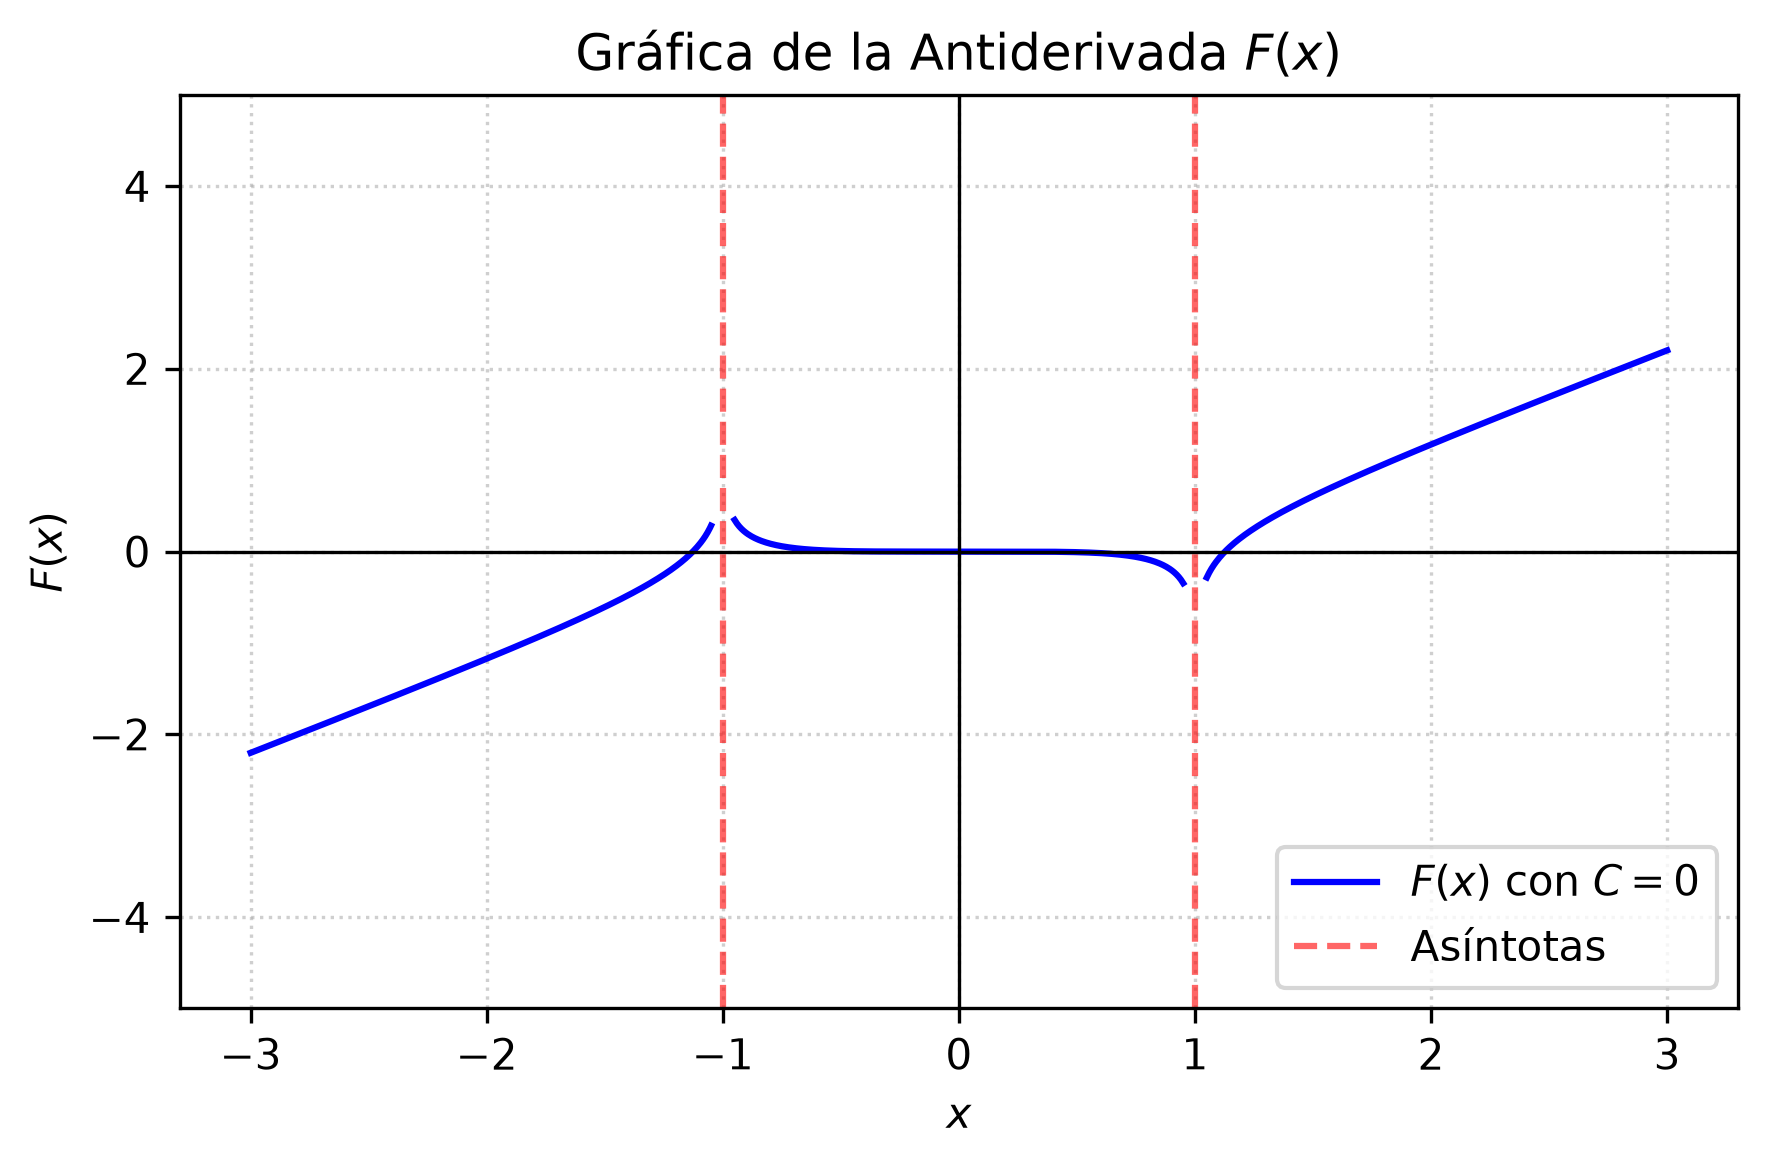
\includegraphics[width=\columnwidth]{semana_03/graficas/SEM03_P12_grafica.png}
	\caption{Representación gráfica de $f(x)$ y su antiderivada $F(x)$ evaluada para la constante de integración $C = 0$ (Problema 12).}
	\label{fig:problema12}
\end{figure}

	\subsection*{Problema 13}
\textbf{Enunciado:} Calcular la integral:
\begin{align*}
\int \dfrac{x^4 - 2x^3 + 3x^2 - x + 3}{x^3 - 2x^2 + 3x} \, dx
\end{align*}

\textbf{Solución:} Dado que el grado del polinomio numerador ($4$) es mayor que el grado del denominador ($3$), realizamos la división algebraica. Dividiendo el numerador entre el denominador:
\begin{align*}
\dfrac{x^4 - 2x^3 + 3x^2 - x + 3}{x^3 - 2x^2 + 3x} &= x + \dfrac{-x + 3}{x^3 - 2x^2 + 3x}
\end{align*}

El denominador se puede factorizar como:
\begin{align*}
x^3 - 2x^2 + 3x &= x(x^2 - 2x + 3)
\end{align*}

Aplicamos fracciones parciales al residuo:
\begin{align*}
\dfrac{-x + 3}{x(x^2 - 2x + 3)} &= \dfrac{A}{x} + \dfrac{Bx + C}{x^2 - 2x + 3}
\end{align*}

Multiplicando por el denominador común:
\begin{align*}
-x + 3 &= A(x^2 - 2x + 3) \\
&\quad + (Bx + C)x
\end{align*}

Agrupando términos semejantes:
\begin{align*}
-x + 3 &= (A + B)x^2 \\
&\quad + (-2A + C)x + 3A
\end{align*}

Igualando coeficientes:
\begin{align*}
A + B &= 0 \\
-2A + C &= -1 \\
3A &= 3 \implies A = 1
\end{align*}

Sustituyendo $A = 1$:
\begin{align*}
1 + B = 0 &\implies B = -1 \\
-2(1) + C = -1 &\implies C = 1
\end{align*}

Sustituyendo las fracciones parciales obtenidas:
\begin{align*}
\dfrac{-x + 3}{x^3 - 2x^2 + 3x} &= \dfrac{1}{x} + \dfrac{-x + 1}{x^2 - 2x + 3}
\end{align*}

Reintegrando toda la expresión:
\begin{align*}
\int \left( x + \dfrac{1}{x} - \dfrac{x - 1}{x^2 - 2x + 3} \right) dx
\end{align*}

Para la última integral, completamos la derivada del denominador en el numerador:
\begin{align*}
\dfrac{x - 1}{x^2 - 2x + 3} &= \dfrac{1}{2}\dfrac{2x - 2}{x^2 - 2x + 3}
\end{align*}

Integrando cada término:
\begin{align*}
\int x \, dx &= \dfrac{x^2}{2} \\
\int \dfrac{1}{x} \, dx &= \ln|x| \\
\int \dfrac{x - 1}{x^2 - 2x + 3} \, dx &= \dfrac{1}{2}\ln|x^2 - 2x + 3|
\end{align*}

Finalmente, la solución general de la integral es:
\begin{align*}
F(x) &= \dfrac{x^2}{2} + \ln|x| \\
&\quad - \dfrac{1}{2}\ln|x^2 - 2x + 3| + C
\end{align*}

\begin{figure}[H]
	\centering
	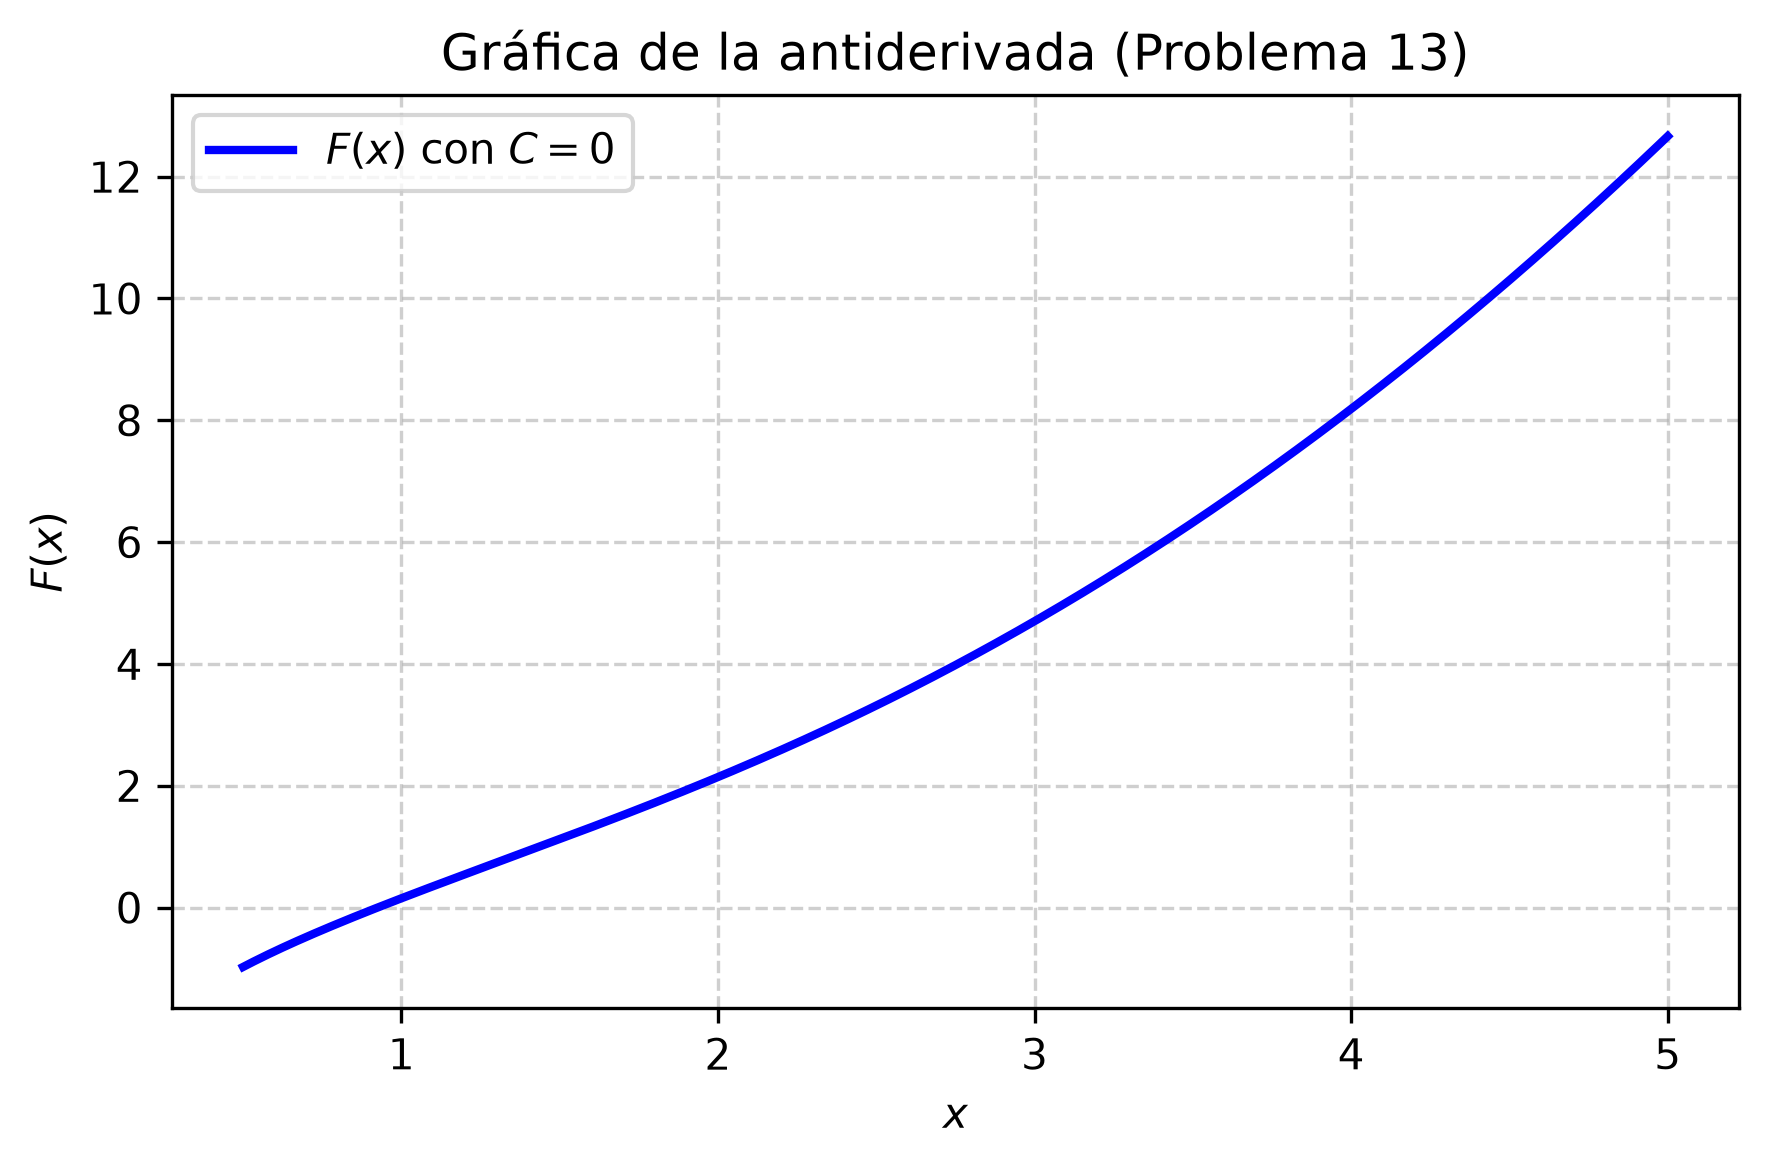
\includegraphics[width=\columnwidth]{semana_03/graficas/SEM03_P13_grafica.png}
	\caption{Representación gráfica de $f(x)$ y su antiderivada $F(x)$ evaluada para la constante de integración $C = 0$ (Problema 13).}
	\label{fig:problema13}
\end{figure}

	\subsection*{Problema 14}

\textbf{Enunciado:} Calcular la integral:
\begin{align*}
\int \dfrac{x^5 + 2}{x^2 - 1} \, dx
\end{align*}

\textbf{Solución:} Dado que el grado del numerador ($5$) es mayor que el grado del denominador ($2$), realizamos la división polinómica de $x^5 + 2$ entre $x^2 - 1$. 

Dividiendo $x^5$ entre $x^2$, obtenemos $x^3$. Multiplicando y restando, continuamos el proceso hasta obtener el cociente y el residuo indicado:
\begin{align*}
\dfrac{x^5 + 2}{x^2 - 1} = x^3 + x + \dfrac{x + 2}{x^2 - 1}
\end{align*}

Sustituimos esta expresión en la integral original:
\begin{align*}
\int \dfrac{x^5 + 2}{x^2 - 1} \, dx = &\int \left( x^3 + x + \dfrac{x + 2}{x^2 - 1} \right) dx \\
= &\int x^3 \, dx + \int x \, dx \\
&+ \int \dfrac{x + 2}{x^2 - 1} \, dx
\end{align*}

Para la tercera integral, descomponemos el integrando en fracciones parciales:
\begin{align*}
\dfrac{x + 2}{x^2 - 1} = \dfrac{x + 2}{(x-1)(x+1)} = \dfrac{A}{x-1} + \dfrac{B}{x+1}
\end{align*}

Resolviendo para los coeficientes $A$ y $B$, encontramos que $A = \frac{3}{2}$ y $B = -\frac{1}{2}$. Por lo tanto:
\begin{align*}
\dfrac{x + 2}{x^2 - 1} = \dfrac{3}{2(x-1)} - \dfrac{1}{2(x+1)}
\end{align*}

Integramos cada término por separado:
\begin{align*}
\int x^3 \, dx &= \dfrac{x^4}{4} \\
\int x \, dx &= \dfrac{x^2}{2} \\
\int \dfrac{\frac{3}{2}}{x-1} \, dx &= \dfrac{3}{2} \ln|x-1| \\
\int \dfrac{-\frac{1}{2}}{x+1} \, dx &= -\dfrac{1}{2} \ln|x+1|
\end{align*}

Agrupando todos los resultados y añadiendo la constante de integración $C$, obtenemos la solución general:
\begin{align*}
F(x) = &\dfrac{x^4}{4} + \dfrac{x^2}{2} + \dfrac{3}{2} \ln|x-1| \\
&- \dfrac{1}{2} \ln|x+1| + C
\end{align*}

\begin{figure}[H]
	\centering
	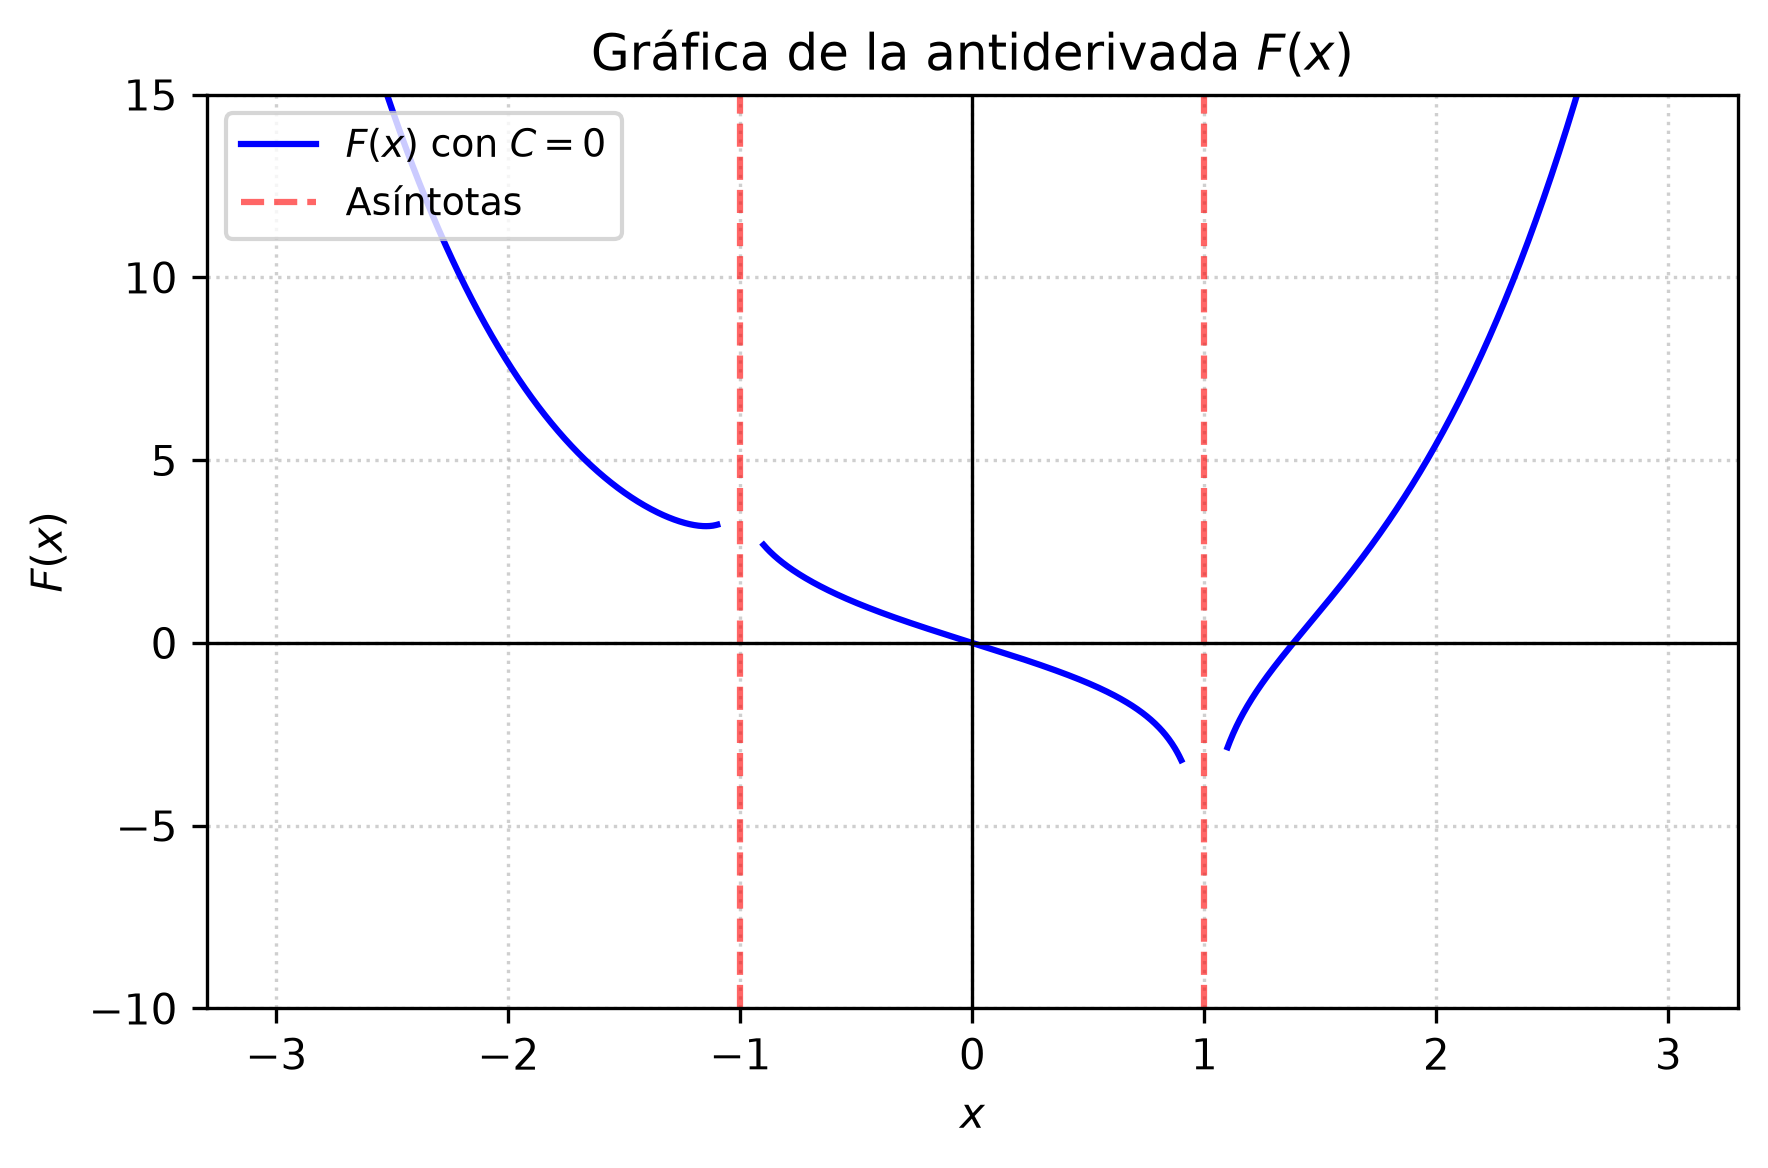
\includegraphics[width=\columnwidth]{semana_03/graficas/SEM03_P14_grafica.png}
	\caption{Representación gráfica de $f(x)$ y su antiderivada $F(x)$ evaluada para la constante de integración $C = 0$ (Problema 14).}
	\label{fig:problema14}
\end{figure}

	\subsection*{Problema 15}

\textbf{Enunciado:}
Calcular la integral indefinida:
\begin{equation*}
\int \dfrac{x^3}{x^2 - 2x - 3} \, dx
\end{equation*}

\textbf{Solución:}
Como el grado del numerador ($3$) es mayor que el grado del denominador ($2$), realizamos primero la división polinómica de $x^3$ entre $x^2 - 2x - 3$.

Dividiendo $x^3$ por $x^2 - 2x - 3$, obtenemos un cociente de $x + 2$ y un residuo de $7x + 6$. Así, el integrando se reescribe como:
\begin{equation*}
\dfrac{x^3}{x^2 - 2x - 3} = x + 2 + \dfrac{7x + 6}{x^2 - 2x - 3}
\end{equation*}

Factorizando el denominador según las indicaciones:
\begin{equation*}
x^2 - 2x - 3 = (x - 3)(x + 1)
\end{equation*}

Aplicamos fracciones parciales al término restante:
\begin{equation*}
\dfrac{7x + 6}{(x - 3)(x + 1)} = \dfrac{A}{x - 3} + \dfrac{B}{x + 1}
\end{equation*}

Multiplicando por el denominador común:
\begin{equation*}
7x + 6 = A(x + 1) + B(x - 3)
\end{equation*}

Si $x = 3$:
\begin{equation*}
7(3) + 6 = A(4) \implies 27 = 4A \implies A = \dfrac{27}{4}
\end{equation*}

Si $x = -1$:
\begin{equation*}
7(-1) + 6 = B(-4) \implies -1 = -4B \implies B = \dfrac{1}{4}
\end{equation*}

Sustituyendo los valores de $A$ y $B$, la integral original se divide en:
\begin{multline*}
\int \dfrac{x^3}{x^2 - 2x - 3} \, dx = \int \left( x + 2 \right) dx \\
+ \int \dfrac{27/4}{x - 3} \, dx + \int \dfrac{1/4}{x + 1} \, dx
\end{multline*}

Integrando cada término por separado, obtenemos la solución general:
\begin{multline*}
\int \dfrac{x^3}{x^2 - 2x - 3} \, dx = \dfrac{x^2}{2} + 2x \\
+ \dfrac{27}{4} \ln|x - 3| + \dfrac{1}{4} \ln|x + 1| + C
\end{multline*}

\begin{figure}[H]
	\centering
	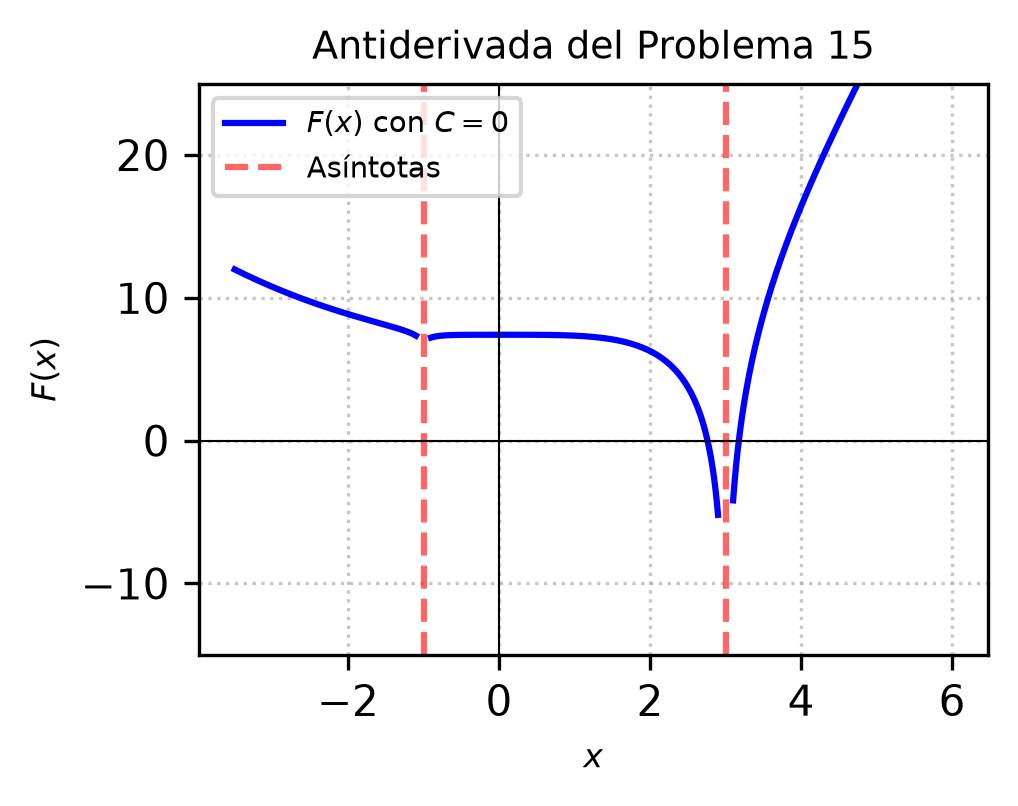
\includegraphics[width=\columnwidth]{semana_03/graficas/SEM03_P15_grafica.png}
	\caption{Representación gráfica de $f(x)$ y su antiderivada $F(x)$ evaluada para la constante de integración $C = 0$ (Problema 15).}
	\label{fig:problema15}
\end{figure}

	\subsection*{Problema 16}

\noindent\textbf{Enunciado:} \\
Calcular la integral indefinida:
\begin{align*}
\int \dfrac{x^2 + 1}{x^3 + 1} \, dx
\end{align*}

\noindent\textbf{Solución:} \\
Primero, factorizamos el denominador utilizando la fórmula de la suma de cubos $x^3 + 1 = (x + 1)(x^2 - x + 1)$:
\begin{align*}
\dfrac{x^2 + 1}{x^3 + 1} = \dfrac{x^2 + 1}{(x + 1)(x^2 - x + 1)}
\end{align*}

Aplicamos el método de fracciones parciales planteando la siguiente identidad:
\begin{align*}
\dfrac{x^2 + 1}{(x + 1)(x^2 - x + 1)} = \dfrac{A}{x + 1} + \dfrac{Bx + C}{x^2 - x + 1}
\end{align*}

Multiplicando ambos lados por el denominador común:
\begin{align*}
x^2 + 1 = A(x^2 - x + 1) \\
+ (Bx + C)(x + 1)
\end{align*}

Agrupando términos según las potencias de $x$:
\begin{align*}
x^2 + 1 = (A + B)x^2 \\
+ (-A + B + C)x + (A + C)
\end{align*}

Igualando los coeficientes de ambos lados de la ecuación, obtenemos el sistema:
\begin{align*}
A + B &= 1 \\
-A + B + C &= 0 \\
A + C &= 1
\end{align*}

Resolviendo el sistema, encontramos que:
\begin{align*}
A = \dfrac{2}{3}, \quad B = \dfrac{1}{3}, \quad C = \dfrac{1}{3}
\end{align*}

Sustituyendo los valores en las fracciones parciales, la integral se divide en dos partes:
\begin{align*}
\int \dfrac{x^2 + 1}{x^3 + 1} \, dx = \int \dfrac{2/3}{x + 1} \, dx \\
+ \int \dfrac{\frac{1}{3}x + \frac{1}{3}}{x^2 - x + 1} \, dx
\end{align*}

Resolvemos la primera integral directamente:
\begin{align*}
\int \dfrac{2/3}{x + 1} \, dx = \dfrac{2}{3} \ln|x + 1|
\end{align*}

Para la segunda integral, ajustamos el numerador para que sea la derivada del denominador ($2x - 1$):
\begin{align*}
\int \dfrac{\frac{1}{3}(x + 1)}{x^2 - x + 1} \, dx = \dfrac{1}{6} \int \dfrac{2x + 2}{x^2 - x + 1} \, dx \\
= \dfrac{1}{6} \int \dfrac{(2x - 1) + 3}{x^2 - x + 1} \, dx
\end{align*}

Separamos en dos integrales:
\begin{align*}
= \dfrac{1}{6} \int \dfrac{2x - 1}{x^2 - x + 1} \, dx \\
+ \dfrac{1}{2} \int \dfrac{1}{\left(x - \frac{1}{2}\right)^2 + \frac{3}{4}} \, dx
\end{align*}

La primera se resuelve por sustitución logarítmica y la segunda mediante la fórmula del arco tangente:
\begin{align*}
= \dfrac{1}{6} \ln|x^2 - x + 1| \\
+ \dfrac{1}{2} \left( \dfrac{2}{\sqrt{3}} \arctan\left(\dfrac{2x - 1}{\sqrt{3}}\right) \right)
\end{align*}

Combinando todos los resultados y agregando la constante de integración $C$, la solución general es:
\begin{align*}
\int \dfrac{x^2 + 1}{x^3 + 1} \, dx = \dfrac{2}{3} \ln|x + 1| \\
+ \dfrac{1}{6} \ln|x^2 - x + 1| \\
+ \dfrac{\sqrt{3}}{3} \arctan\left(\dfrac{2x - 1}{\sqrt{3}}\right) + C
\end{align*}

\begin{figure}[H]
	\centering
	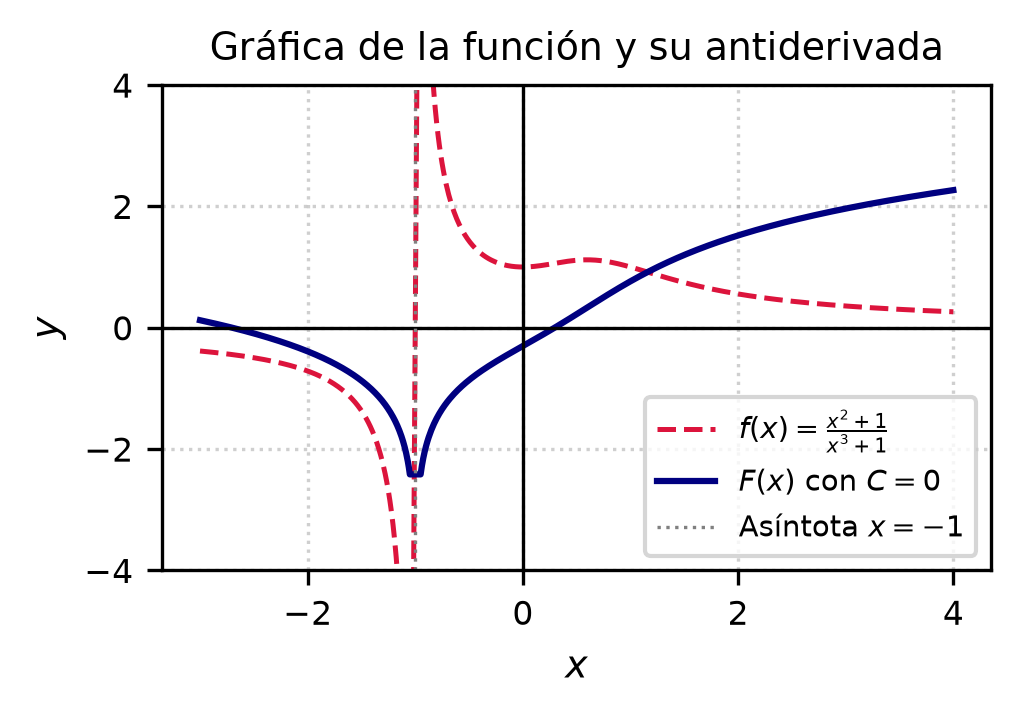
\includegraphics[width=\columnwidth]{semana_03/graficas/SEM03_P16_grafica.png}
	\caption{Representación gráfica de $f(x)$ y su antiderivada $F(x)$ evaluada para la constante de integración $C = 0$ (Problema 16).}
	\label{fig:problema16}
\end{figure}

	\subsection*{Problema 17}

\textbf{Enunciado:} Calcular la integral indefinida
\begin{align*}
\int \dfrac{x^2 + 6}{(x - 1)^2 (x - 2)} \, dx
\end{align*}

\textbf{Solución:} 
Utilizamos el método de fracciones parciales. La forma sugerida es:
\begin{align*}
\dfrac{x^2 + 6}{(x - 1)^2 (x - 2)} = \dfrac{A}{x - 1} + \dfrac{B}{(x - 1)^2} + \dfrac{C}{x - 2}
\end{align*}

Multiplicamos toda la expresión por el denominador común $(x - 1)^2 (x - 2)$:
\begin{align*}
x^2 + 6 = \, & A(x - 1)(x - 2) \\
& + B(x - 2) + C(x - 1)^2
\end{align*}

Para hallar las constantes, evaluamos en valores convenientes de $x$:

Si $x = 1$:
\begin{align*}
1^2 + 6 &= B(1 - 2) \\
7 &= -B \implies B = -7
\end{align*}

Si $x = 2$:
\begin{align*}
2^2 + 6 &= C(2 - 1)^2 \\
10 &= C(1)^2 \implies C = 10
\end{align*}

Para hallar $A$, evaluamos en $x = 0$ y usamos $B = -7, C = 10$:
\begin{align*}
0^2 + 6 &= A(-1)(-2) + B(-2) + C(-1)^2 \\
6 &= 2A - 2(-7) + 10(1) \\
6 &= 2A + 14 + 10 \implies 2A = -18 \\
A &= -9
\end{align*}

Sustituimos las constantes en la integral:
\begin{align*}
\int \dfrac{x^2 + 6}{(x - 1)^2 (x - 2)} \, dx = \, & \int \left( \dfrac{-9}{x - 1} \right) dx \\
& + \int \left( \dfrac{-7}{(x - 1)^2} \right) dx \\
& + \int \left( \dfrac{10}{x - 2} \right) dx
\end{align*}

Resolvemos cada integral por separado:
\begin{align*}
\int \dfrac{-9}{x - 1} \, dx &= -9 \ln |x - 1| \\
\int \dfrac{-7}{(x - 1)^2} \, dx &= \dfrac{7}{x - 1} \\
\int \dfrac{10}{x - 2} \, dx &= 10 \ln |x - 2|
\end{align*}

Agrupando los resultados y añadiendo la constante de integración $C$, obtenemos la solución general:
\begin{align*}
F(x) = \, & 10 \ln |x - 2| - 9 \ln |x - 1| \\
& + \dfrac{7}{x - 1} + C
\end{align*}

\begin{figure}[H]
	\centering
	
\includegraphics[width=\columnwidth]{semana_03/graficas/SEM03_P17_grafica.png}
	\caption{Representación gráfica de $f(x)$ y su antiderivada $F(x)$ evaluada para la constante de integración $C = 0$ (Problema 17).}
	\label{fig:problema17}
\end{figure}

	\subsection*{Problema 18}

\textbf{Enunciado:} Calcular la integral:
\begin{align*}
\int \dfrac{x^2 - 1}{(x^2 + 1)(x - 2)} \, dx
\end{align*}

\textbf{Solución:} \\
Utilizamos el método de fracciones parciales. 
Planteamos la descomposición indicada:
\begin{align*}
\dfrac{x^2 - 1}{(x^2 + 1)(x - 2)} &= \dfrac{Ax + B}{x^2 + 1} + \dfrac{C}{x - 2}
\end{align*}

Multiplicando ambos lados por el denominador común:
\begin{multline*}
x^2 - 1 = (Ax + B)(x - 2) \\
+ C(x^2 + 1)
\end{multline*}

Expandimos el miembro derecho:
\begin{multline*}
x^2 - 1 = Ax^2 - 2Ax + Bx \\
- 2B + Cx^2 + C
\end{multline*}

Agrupamos términos según las potencias de $x$:
\begin{multline*}
x^2 - 1 = (A + C)x^2 \\
+ (-2A + B)x + (-2B + C)
\end{multline*}

Igualamos los coeficientes:
\begin{align*}
A + C &= 1 \\
-2A + B &= 0 \\
-2B + C &= -1
\end{align*}

De la segunda ecuación, $B = 2A$. 
Sustituyendo $C = 1 - A$ y $B = 2A$ en la tercera:
\begin{align*}
-2(2A) + (1 - A) &= -1 \\
-4A + 1 - A &= -1 \\
-5A &= -2 \implies A = \dfrac{2}{5}
\end{align*}

Calculamos $B$ y $C$:
\begin{align*}
B &= 2\left(\dfrac{2}{5}\right) = \dfrac{4}{5} \\
C &= 1 - \dfrac{2}{5} = \dfrac{3}{5}
\end{align*}

Sustituimos los coeficientes:
\begin{multline*}
\int \dfrac{x^2 - 1}{(x^2 + 1)(x - 2)} \, dx = 
\int \dfrac{\frac{2}{5}x + \frac{4}{5}}{x^2 + 1} \, dx \\
+ \int \dfrac{\frac{3}{5}}{x - 2} \, dx
\end{multline*}

Resolvemos cada integral por separado:
\begin{align*}
&= \dfrac{1}{5} \int \dfrac{2x}{x^2 + 1} \, dx \\
&\quad + \dfrac{4}{5} \int \dfrac{1}{x^2 + 1} \, dx \\
&\quad + \dfrac{3}{5} \int \dfrac{1}{x - 2} \, dx
\end{align*}

Integrando cada término:
\begin{multline*}
= \dfrac{1}{5} \ln|x^2 + 1| \\
+ \dfrac{4}{5} \arctan(x) \\
+ \dfrac{3}{5} \ln|x - 2| + K
\end{multline*}

La solución general de la integral es:
\begin{multline*}
F(x) = \dfrac{1}{5} \ln(x^2 + 1) \\
+ \dfrac{4}{5} \arctan(x) \\
+ \dfrac{3}{5} \ln|x - 2| + C
\end{multline*}

\begin{figure}[H]
	\centering
	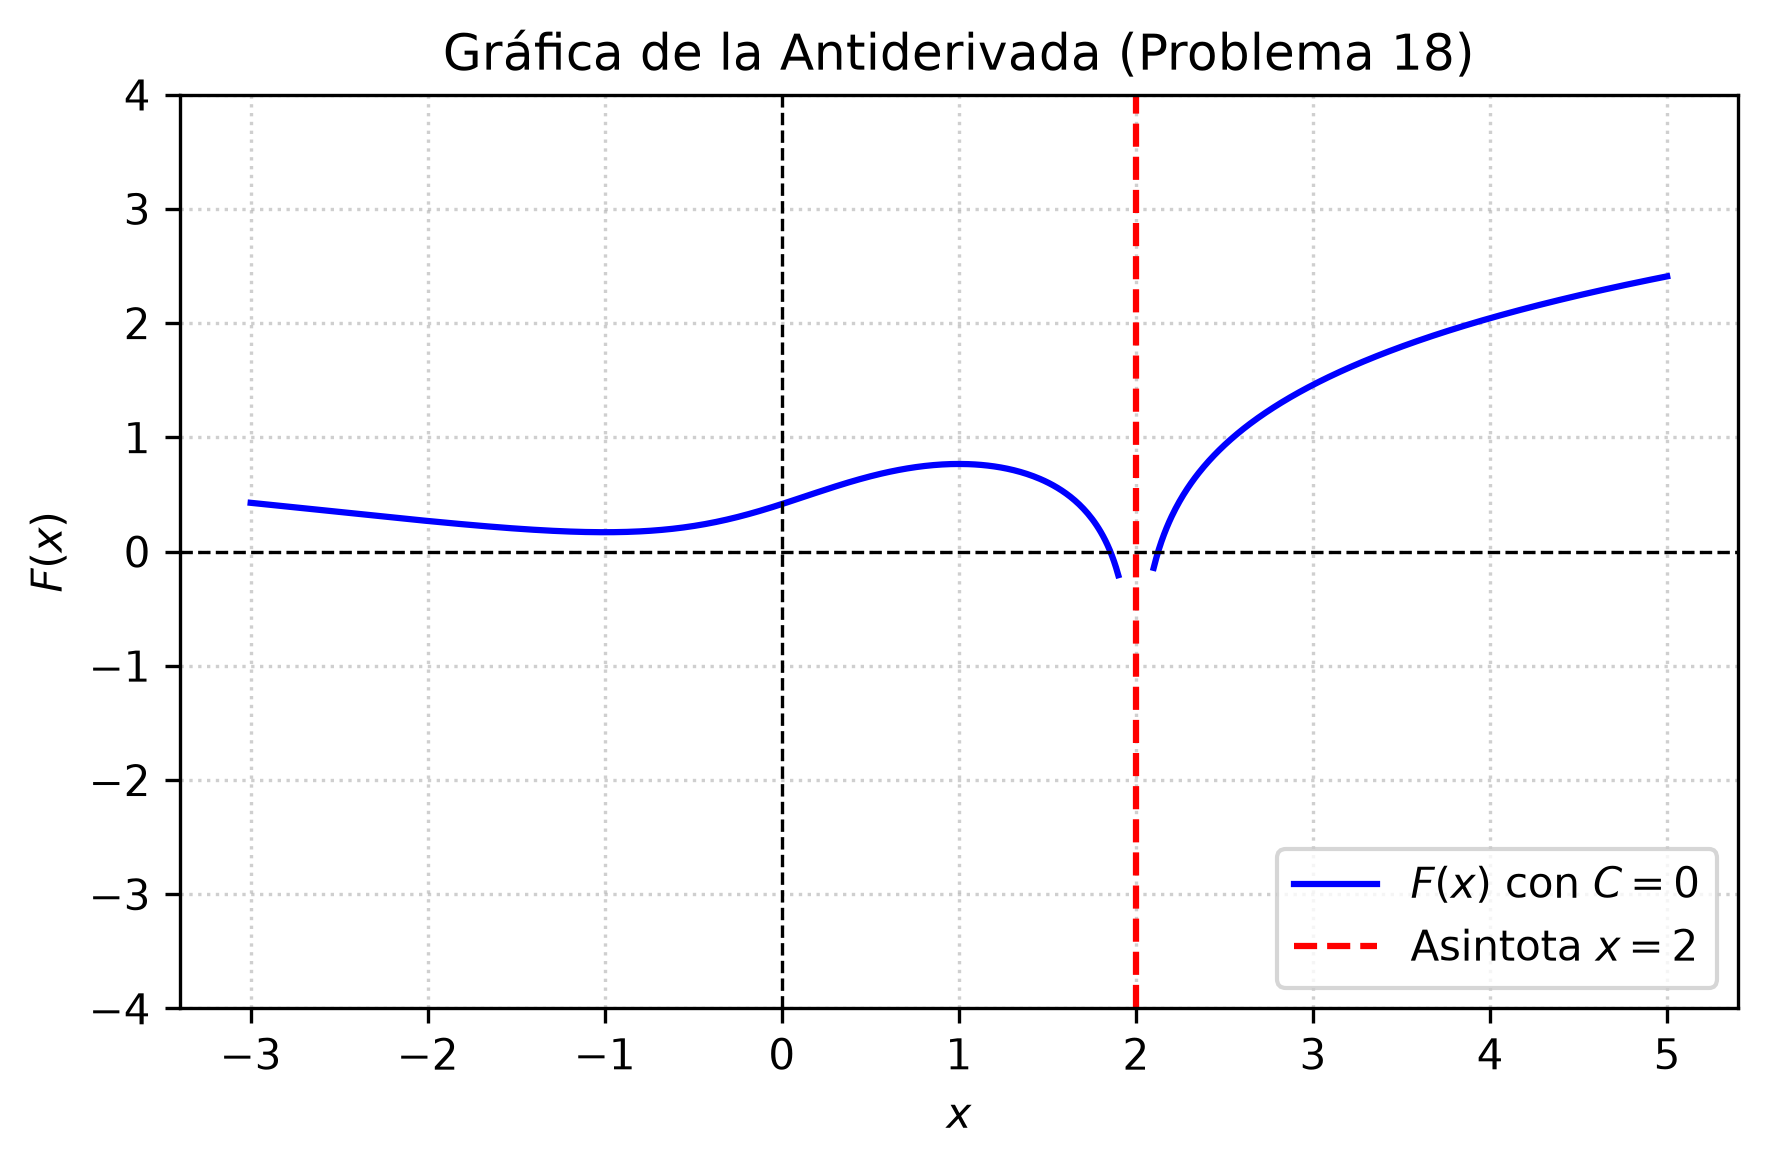
\includegraphics[width=\columnwidth]{semana_03/graficas/SEM03_P18_grafica.png}
	\caption{Representación gráfica de $f(x)$ y su antiderivada $F(x)$ evaluada para la constante de integración $C = 0$ (Problema 18).}
	\label{fig:problema18}
\end{figure}

	\subsection*{Problema 19}
\textbf{Enunciado:} Calcular la integral:
\begin{equation*}
\int \frac{3x^2 + 2x - 2}{x^3 - 1} \, dx
\end{equation*}

\textbf{Solución:} 
Utilizamos la descomposición en fracciones parciales. El denominador se factoriza como:
\begin{equation*}
x^3 - 1 = (x - 1)(x^2 + x + 1)
\end{equation*}

Planteamos la forma de las fracciones parciales:
\begin{multline*}
\frac{3x^2 + 2x - 2}{x^3 - 1} = \frac{A}{x - 1} \\
+ \frac{Bx + C}{x^2 + x + 1}
\end{multline*}

Multiplicando por el denominador común:
\begin{multline*}
3x^2 + 2x - 2 = A(x^2 + x + 1) \\
+ (Bx + C)(x - 1)
\end{multline*}

Evaluamos en $x = 1$ para hallar $A$:
\begin{equation*}
3(1)^2 + 2(1) - 2 = A(1^2 + 1 + 1)
\end{equation*}
\begin{equation*}
3 = 3A \implies A = 1
\end{equation*}

Expandimos y agrupamos términos según las potencias de $x$:
\begin{multline*}
3x^2 + 2x - 2 = (A + B)x^2 \\
+ (A - B + C)x + (A - C)
\end{multline*}

Igualando coeficientes:
\begin{align*}
A + B &= 3 \\
A - B + C &= 2 \\
A - C &= -2
\end{align*}

Como $A = 1$, obtenemos $B = 2$ y $C = 3$. La integral se reescribe como:
\begin{equation*}
\int \left( \frac{1}{x - 1} + \frac{2x + 3}{x^2 + x + 1} \right) dx
\end{equation*}

Para el segundo término, ajustamos el numerador para que sea la derivada del denominador ($2x + 1$):
\begin{multline*}
\int \frac{2x + 3}{x^2 + x + 1} \, dx = \int \frac{2x + 1}{x^2 + x + 1} \, dx \\
+ \int \frac{2}{x^2 + x + 1} \, dx
\end{multline*}

Completando el cuadrado en el último término:
\begin{equation*}
x^2 + x + 1 = \left(x + \frac{1}{2}\right)^2 + \frac{3}{4}
\end{equation*}

Integramos cada parte:
\begin{multline*}
\int \frac{3x^2 + 2x - 2}{x^3 - 1} \, dx = \ln|x - 1| \\
+ \ln|x^2 + x + 1| \\
+ \frac{2}{\frac{\sqrt{3}}{2}} \arctan\left(\frac{x + \frac{1}{2}}{\frac{\sqrt{3}}{2}}\right) + C
\end{multline*}

Simplificando el resultado final:
\begin{multline*}
= \ln|x^3 - 1| \\
+ \frac{4}{\sqrt{3}} \arctan\left(\frac{2x + 1}{\sqrt{3}}\right) + C
\end{multline*}

\begin{figure}[H]
	\centering
	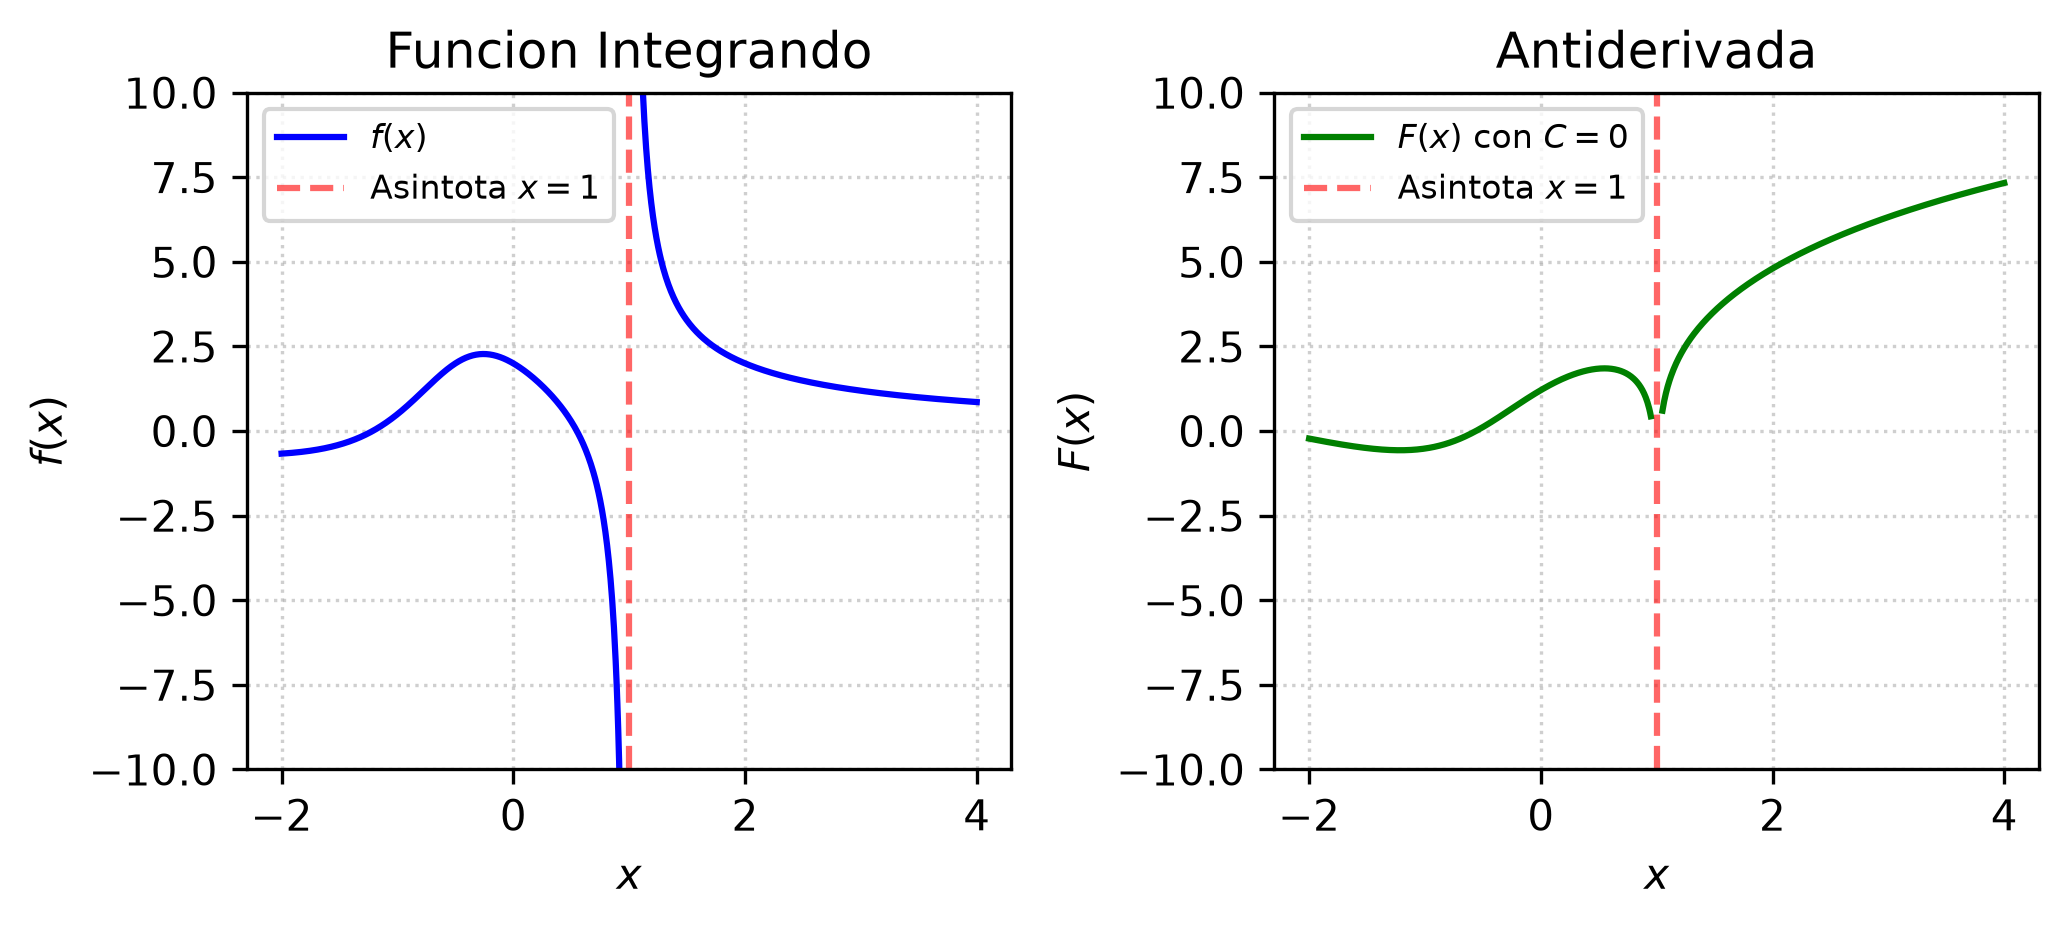
\includegraphics[width=\columnwidth]{semana_03/graficas/SEM03_P19_grafica.png}
	\caption{Representación gráfica de $f(x)$ y su antiderivada $F(x)$ evaluada para la constante de integración $C = 0$ (Problema 19).}
	\label{fig:problema19}
\end{figure}

	\subsection*{Problema 20}

\textbf{Enunciado:}
Calcular la integral:
\begin{align*}
\int \dfrac{x^4 - x^3 - 2x^2 - x + 2}{(x - 1)(x^2 + 2)^2} \, dx
\end{align*}

\textbf{Solución:}
El integrando es una función racional propia. 
Aplicamos fracciones parciales con un 
factor cuadrático repetido:
\begin{align*}
\dfrac{x^4 - x^3 - 2x^2 - x + 2}{(x - 1)(x^2 + 2)^2} &= 
\dfrac{A}{x - 1} \\
&+ \dfrac{Bx + C}{x^2 + 2} \\
&+ \dfrac{Dx + E}{(x^2 + 2)^2}
\end{align*}

Multiplicando por el denominador común 
$(x - 1)(x^2 + 2)^2$ y agrupando términos, 
obtenemos los coeficientes:
\begin{align*}
A &= 0, \quad B = 1, \quad C = 0, \\
D &= -1, \quad E = -1
\end{align*}

Sustituyendo los coeficientes:
\begin{align*}
\int &\dfrac{x}{(x^2 + 2)} \, dx \\
&- \int \dfrac{x + 1}{(x^2 + 2)^2} \, dx
\end{align*}

Para la primera integral, usamos sustitución 
simple $u = x^2 + 2$, $du = 2x \, dx$:
\begin{align*}
\int \dfrac{x}{x^2 + 2} \, dx &= \dfrac{1}{2}\ln|x^2 + 2|
\end{align*}

Para la segunda integral, se descompone:
\begin{align*}
\int \dfrac{x}{(x^2 + 2)^2} \, dx &= -\dfrac{1}{2(x^2 + 2)}
\end{align*}

Y para $\int \dfrac{1}{(x^2 + 2)^2} \, dx$, 
aplicamos la sustitución trigonométrica 
$x = \sqrt{2}\tan(\theta)$:
\begin{align*}
\int &\dfrac{\sqrt{2}\sec^2(\theta)}{4\sec^4(\theta)} \, d\theta \\
&= \dfrac{\sqrt{2}}{4} \int \cos^2(\theta) \, d\theta \\
&= \dfrac{\sqrt{2}}{8}(\theta + \sin(\theta)\cos(\theta))
\end{align*}

Volviendo a la variable original $x$:
\begin{align*}
\int &\dfrac{1}{(x^2 + 2)^2} \, dx \\
&= \dfrac{x}{4(x^2 + 2)} + \dfrac{\sqrt{2}}{8}\arctan\left(\dfrac{x}{\sqrt{2}}\right)
\end{align*}

Agrupando todos los resultados y la 
constante de integración $C$:
\begin{align*}
F(x) &= \dfrac{1}{2}\ln(x^2 + 2) 
+ \dfrac{1}{4(x^2 + 2)} \\
&- \dfrac{x}{4(x^2 + 2)} 
- \dfrac{\sqrt{2}}{8}\arctan\left(\dfrac{x}{\sqrt{2}}\right) + C
\end{align*}

\begin{figure}[H]
	\centering
	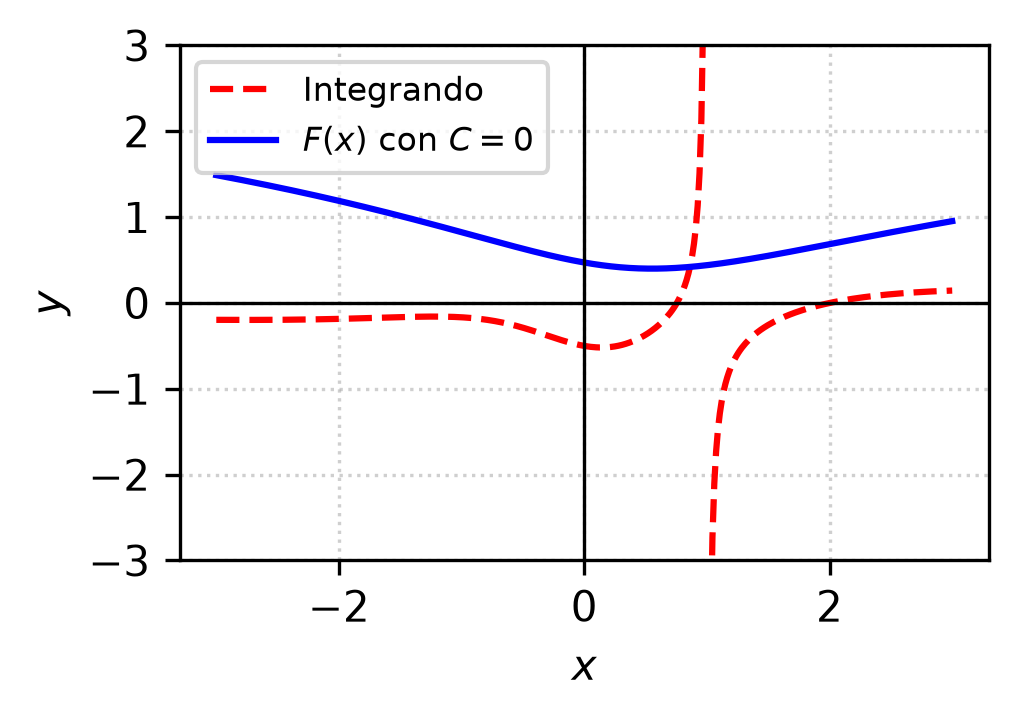
\includegraphics[width=\columnwidth]{semana_03/graficas/SEM03_P20_grafica.png}
	\caption{Representación gráfica de $f(x)$ y su antiderivada $F(x)$ evaluada para la constante de integración $C = 0$ (Problema 20).}
	\label{fig:problema20}
\end{figure}

	\subsection*{Problema 21}
\textbf{Enunciado:} Calcular la integral:
\begin{equation*}
\int \dfrac{2x^2 - 7x - 1}{x^3 + x^2 - x - 1} \, dx
\end{equation*}

\textbf{Solución:} Analizamos el denominador
de la función racional para factorizarlo
por agrupación de términos:
\begin{align*}
x^3 + x^2 - x - 1 &= x^2(x + 1) - (x + 1) \\
&= (x + 1)(x^2 - 1) \\
&= (x + 1)^2(x - 1)
\end{align*}

Planteamos la descomposición en
fracciones parciales con factores
repetidos y lineales:
\begin{align*}
\dfrac{2x^2 - 7x - 1}{(x+1)^2(x-1)} &= 
\dfrac{A}{x+1} + \dfrac{B}{(x+1)^2} \\
&\quad + \dfrac{C}{x-1}
\end{align*}

Multiplicamos toda la ecuación por
el denominador común $(x+1)^2(x-1)$:
\begin{align*}
2x^2 - 7x - 1 &= A(x+1)(x-1) \\
&\quad + B(x-1) + C(x+1)^2
\end{align*}

Evaluamos en valores convenientes de $x$:
\begin{align*}
\text{Si } x = 1 &\implies 2(1)^2 - 7(1) - 1 \\
&= C(1+1)^2 \\
-6 &= 4C \implies C = -\dfrac{3}{2}
\end{align*}

\begin{align*}
\text{Si } x = -1 &\implies 2(-1)^2 - 7(-1) - 1 \\
&= B(-1-1) \\
8 &= -2B \implies B = -4
\end{align*}

Para hallar $A$, evaluamos en $x = 0$
y usamos $B = -4$, $C = -\dfrac{3}{2}$:
\begin{align*}
-1 &= A(1)(-1) + B(-1) + C(1)^2 \\
-1 &= -A - B + C \\
-1 &= -A - (-4) - \dfrac{3}{2} \\
-1 &= -A + 4 - \dfrac{3}{2} \implies A = \dfrac{7}{2}
\end{align*}

Sustituimos los coeficientes $A$, $B$ y $C$
en la integral original:
\begin{align*}
&\int \dfrac{2x^2 - 7x - 1}{x^3 + x^2 - x - 1} \, dx = \\
&\int \left( \dfrac{7/2}{x+1} - \dfrac{4}{(x+1)^2} - \dfrac{3/2}{x-1} \right) dx
\end{align*}

Integramos cada término por separado:
\begin{align*}
&= \dfrac{7}{2} \ln|x+1| + \dfrac{4}{x+1} \\
&\quad - \dfrac{3}{2} \ln|x-1| + C
\end{align*}

Agrupamos los logaritmos utilizando las
propiedades correspondientes:
\begin{align*}
&= \dfrac{7}{2} \ln|x+1| - \dfrac{3}{2} \ln|x-1| \\
&\quad + \dfrac{4}{x+1} + C \\
&= \dfrac{1}{2} \ln\left| \dfrac{(x+1)^7}{(x-1)^3} \right| \\
&\quad + \dfrac{4}{x+1} + C
\end{align*}

\begin{figure}[H]
	\centering
	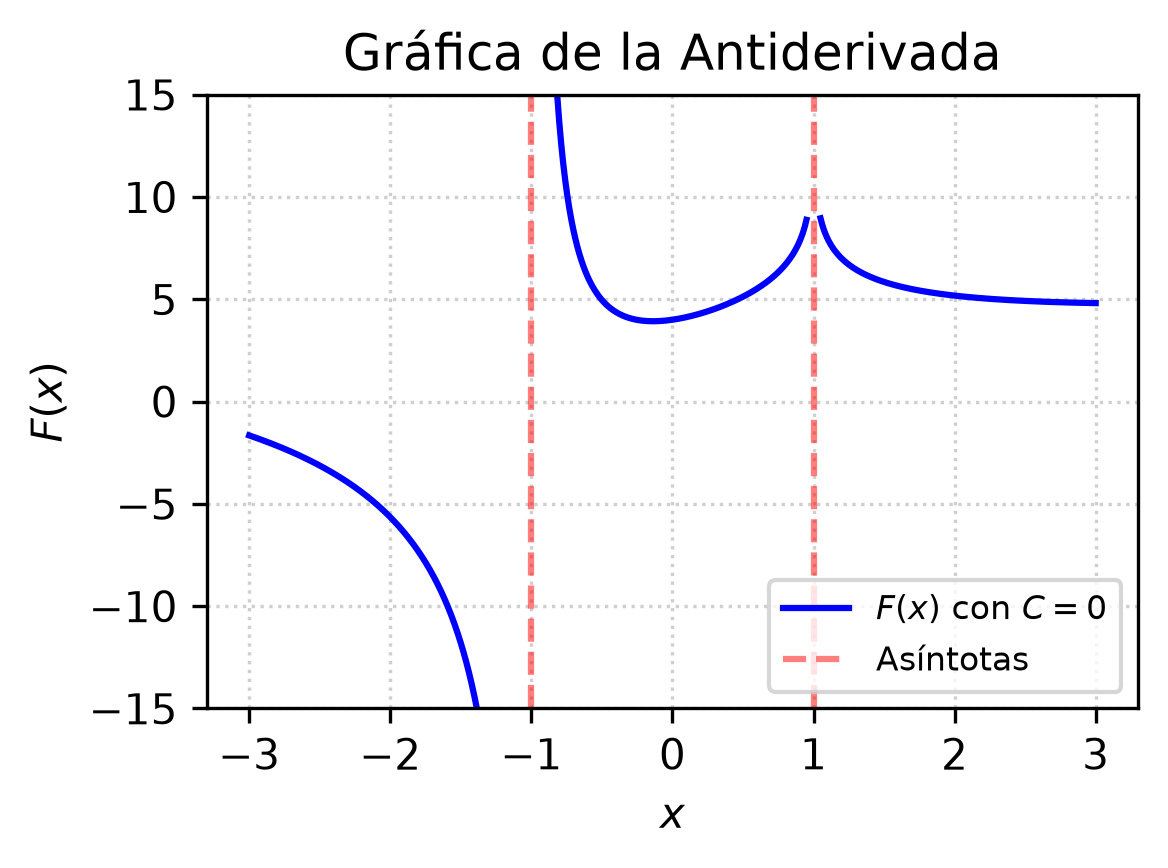
\includegraphics[width=\columnwidth]{semana_03/graficas/SEM03_P21_grafica.png}
	\caption{Representación gráfica de $f(x)$ y su antiderivada $F(x)$ evaluada para la constante de integración $C = 0$ (Problema 21).}
	\label{fig:problema21}
\end{figure}

	\subsection*{Problema 22}
\textbf{Enunciado:} Calcular la integral:
\begin{align*}
\int \dfrac{3x^2 + 3x + 1}{x^3 + 2x^2 + 2x + 1} \, dx
\end{align*}

\textbf{Solución:} 
Primero, factorizamos el denominador agrupando
términos o probando raíces racionales. 
Notamos que $x = -1$ es una raíz de 
$x^3 + 2x^2 + 2x + 1 = 0$. 
Dividiendo entre $x + 1$, obtenemos:
\begin{align*}
x^3 + 2x^2 + 2x + 1 = (x + 1)(x^2 + x + 1)
\end{align*}

Planteamos la descomposición en 
fracciones parciales según se indica:
\begin{align*}
\dfrac{3x^2 + 3x + 1}{(x + 1)(x^2 + x + 1)} = 
\dfrac{A}{x + 1} + \dfrac{Bx + C}{x^2 + x + 1}
\end{align*}

Multiplicando por el denominador común:
\begin{align*}
3x^2 + 3x + 1 &= A(x^2 + x + 1) \\
&\quad + (Bx + C)(x + 1)
\end{align*}

Expandimos y agrupamos términos por potencias de $x$:
\begin{align*}
3x^2 + 3x + 1 &= (A + B)x^2 \\
&\quad + (A + B + C)x + (A + C)
\end{align*}

Igualando los coeficientes de ambos lados:
\begin{align*}
A + B &= 3 \\
A + B + C &= 3 \\
A + C &= 1
\end{align*}

De la primera y segunda ecuación, 
sustituimos $A + B = 3$:
\begin{align*}
3 + C = 3 \implies C = 0
\end{align*}

Sustituyendo $C = 0$ en la tercera ecuación:
\begin{align*}
A + 0 = 1 \implies A = 1
\end{align*}

Y usando $A = 1$ en la primera ecuación:
\begin{align*}
1 + B = 3 \implies B = 2
\end{align*}

Sustituimos los valores de $A$, $B$ y $C$ 
en las fracciones parciales:
\begin{align*}
\int \left( \dfrac{1}{x + 1} + \dfrac{2x}{x^2 + x + 1} \right) dx
\end{align*}

Para la segunda integral, ajustamos el numerador 
para que sea la derivada del denominador 
($\dfrac{d}{dx}(x^2 + x + 1) = 2x + 1$):
\begin{align*}
\int \dfrac{2x}{x^2 + x + 1} dx &= \int \dfrac{2x + 1 - 1}{x^2 + x + 1} dx \\
&= \int \dfrac{2x + 1}{x^2 + x + 1} dx \\
&\quad - \int \dfrac{1}{(x + \frac{1}{2})^2 + \frac{3}{4}} dx
\end{align*}

Integramos cada término resultante:
\begin{align*}
\int \dfrac{1}{x + 1} dx &= \ln|x + 1| \\
\int \dfrac{2x + 1}{x^2 + x + 1} dx &= \ln|x^2 + x + 1| \\
\int \dfrac{1}{(x + \frac{1}{2})^2 + \frac{3}{4}} dx &= \dfrac{2}{\sqrt{3}} \arctan\left(\dfrac{2x + 1}{\sqrt{3}}\right)
\end{align*}

Juntando todas las antiderivadas, 
la solución general es:
\begin{align*}
F(x) &= \ln|x + 1| + \ln|x^2 + x + 1| \\
&\quad - \dfrac{2}{\sqrt{3}} \arctan\left(\dfrac{2x + 1}{\sqrt{3}}\right) + C
\end{align*}
O de forma compacta:
\begin{align*}
F(x) &= \ln|(x + 1)(x^2 + x + 1)| \\
&\quad - \dfrac{2}{\sqrt{3}} \arctan\left(\dfrac{2x + 1}{\sqrt{3}}\right) + C
\end{align*}

\begin{figure}[H]
	\centering
	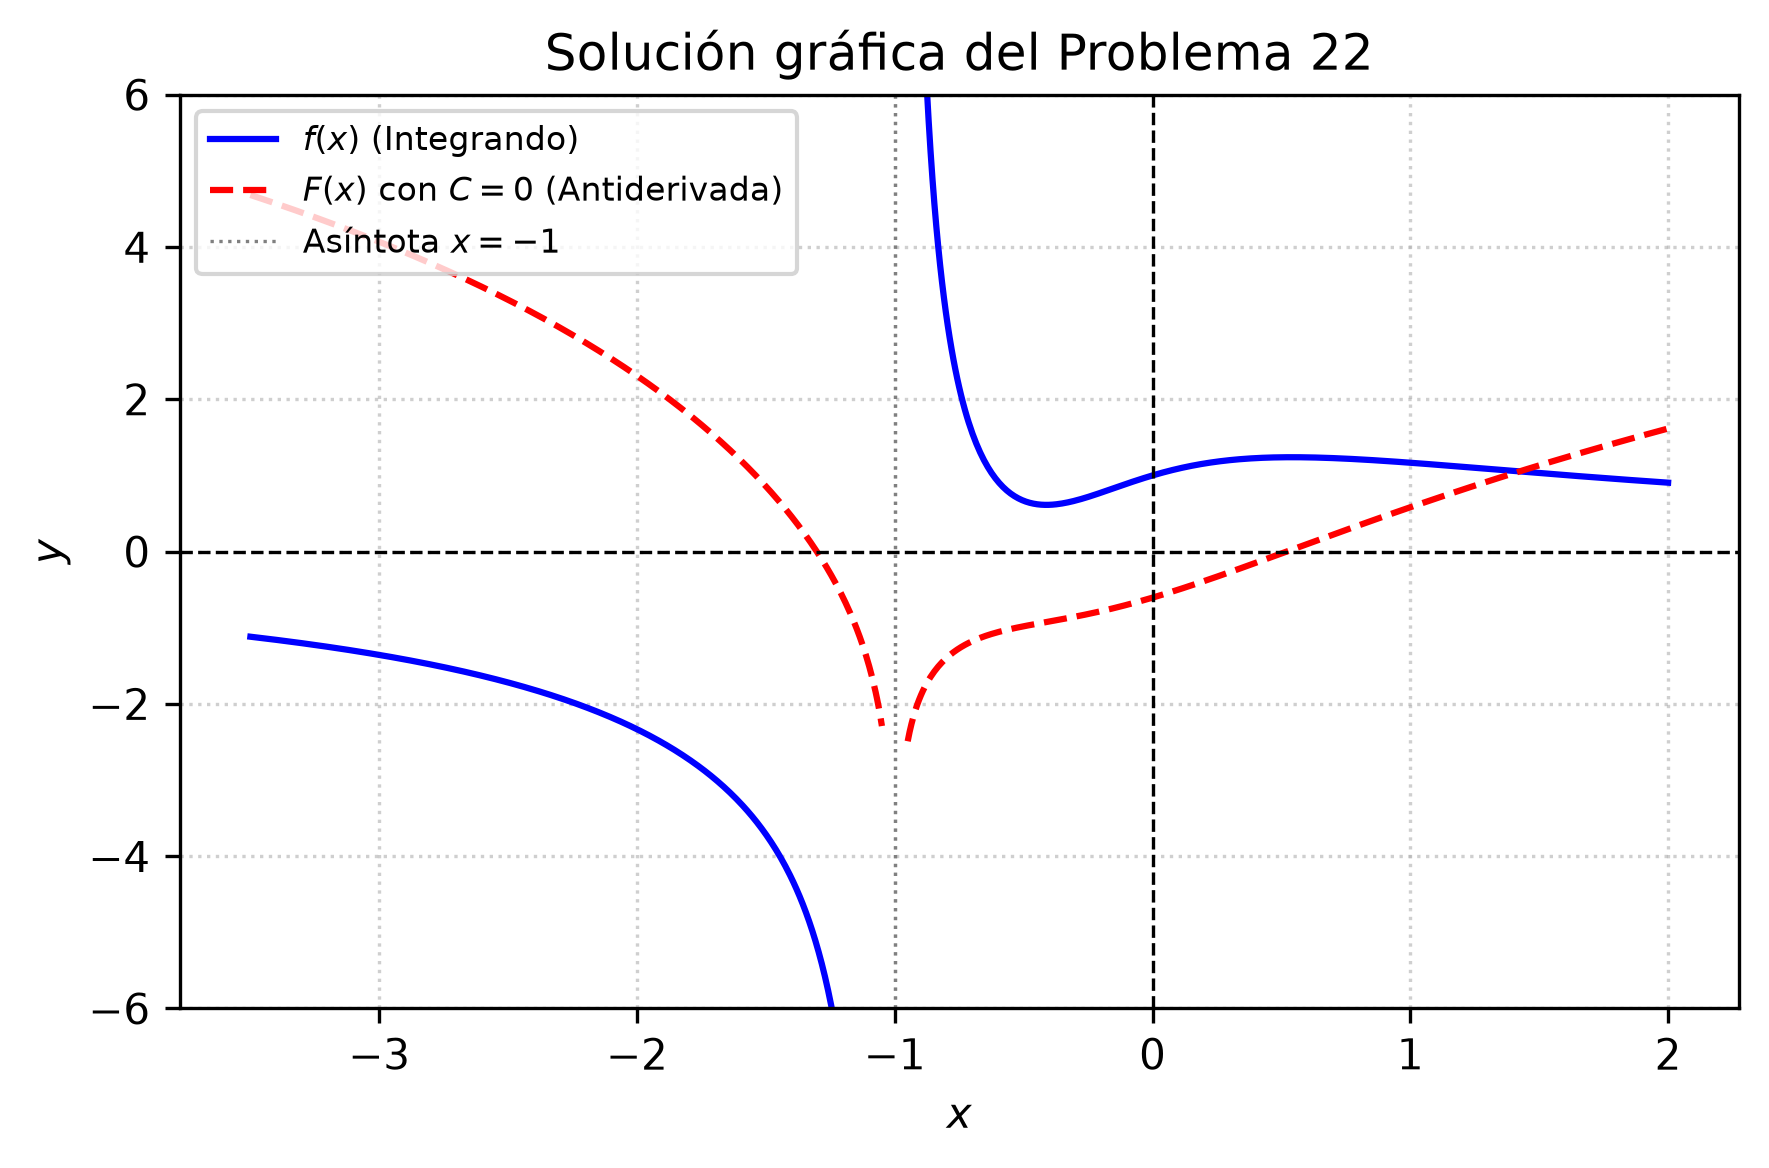
\includegraphics[width=\columnwidth]{semana_03/graficas/SEM03_P22_grafica.png}
	\caption{Representación gráfica de $f(x)$ y su antiderivada $F(x)$ evaluada para la constante de integración $C = 0$ (Problema 22).}
	\label{fig:problema22}
\end{figure}

	\subsection*{Problema 23}

\textbf{Enunciado:} Calcular la integral:
\begin{align*}
\int \dfrac{x^3 + 7x^2 - 5x + 5}{(x - 1)^2 (x^2 + 1)^2} \, dx
\end{align*}

\textbf{Solución:} Proponemos la descomposición en fracciones parciales con factores lineales y cuadráticos repetidos:
\begin{align*}
\dfrac{x^3 + 7x^2 - 5x + 5}{(x - 1)^2 (x^2 + 1)^2} &= \dfrac{A}{x-1} + \dfrac{B}{(x-1)^2} \\
&+ \dfrac{Cx+D}{x^2+1} + \dfrac{Ex+F}{(x^2+1)^2}
\end{align*}

Multiplicando por el denominador común e igualando numeradores, evaluamos en valores convenientes y resolvemos el sistema de ecuaciones para los coeficientes:
\begin{align*}
A &= 1, \quad B = 2, \quad C = -1, \\
D &= 3, \quad E = -2, \quad F = 0
\end{align*}

Reescribimos la integral con las fracciones parciales obtenidas:
\begin{align*}
I &= \int \dfrac{1}{x-1} \, dx + \int \dfrac{2}{(x-1)^2} \, dx \\
&- \int \dfrac{x-3}{x^2+1} \, dx - \int \dfrac{2x}{(x^2+1)^2} \, dx
\end{align*}

Integramos cada término por separado. Las primeras dos integrales son directas:
\begin{align*}
\int \dfrac{1}{x-1} \, dx &= \ln|x-1| \\
\int \dfrac{2}{(x-1)^2} \, dx &= -\dfrac{2}{x-1}
\end{align*}

Para la tercera integral, separamos en términos logarítmicos y trigonométricos (sustitución $x = \tan\theta$):
\begin{align*}
\int \dfrac{x-3}{x^2+1} \, dx &= \int \dfrac{x}{x^2+1} \, dx - 3\int \dfrac{1}{x^2+1} \, dx \\
&= \dfrac{1}{2}\ln(x^2+1) - 3\arctan(x)
\end{align*}

La cuarta integral se resuelve mediante sustitución simple $u = x^2+1$:
\begin{align*}
\int \dfrac{2x}{(x^2+1)^2} \, dx &= -\dfrac{1}{x^2+1}
\end{align*}

Agrupando todos los resultados y añadiendo la constante de integración $C$, obtenemos la solución general:
\begin{align*}
I &= \ln|x-1| - \dfrac{2}{x-1} \\
&- \dfrac{1}{2}\ln(x^2+1) + 3\arctan(x) \\
&+ \dfrac{1}{x^2+1} + C
\end{align*}

\begin{figure}[H]
	\centering
	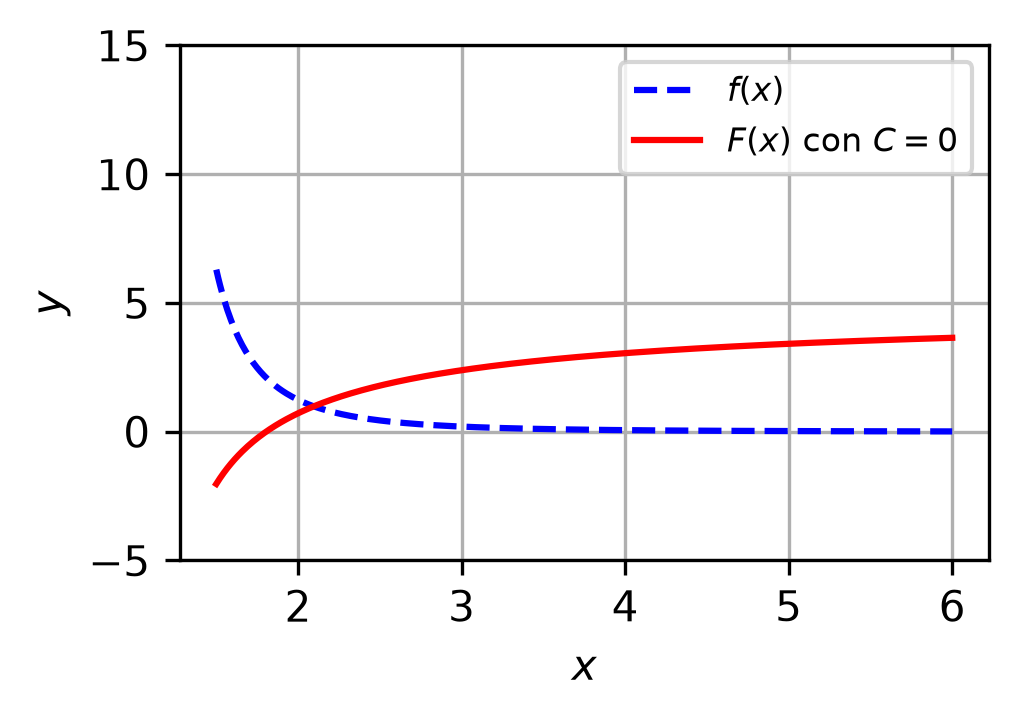
\includegraphics[width=\columnwidth]{semana_03/graficas/SEM03_P23_grafica.png}
	\caption{Representación gráfica de $f(x)$ y su antiderivada $F(x)$ evaluada para la constante de integración $C = 0$ (Problema 23).}
	\label{fig:problema23}
\end{figure}

	\subsection*{Problema 24}

\textbf{Enunciado:} Calcular la integral:
\begin{equation*}
\int \dfrac{2x}{(x^2 + x + 1)^2} dx
\end{equation*}

\textbf{Solución:}

Primero, completamos el cuadrado
en el trinomio del denominador:
\begin{align*}
x^2 + x + 1 &= \left(x + \dfrac{1}{2}\right)^2 + \dfrac{3}{4}
\end{align*}

Reescribimos la integral original
con esta nueva expresión:
\begin{align*}
I &= \int \dfrac{2x}{\left(\left(x + \frac{1}{2}\right)^2 + \frac{3}{4}\right)^2} dx
\end{align*}

Aplicamos la sustitución trigonométrica
sugerida:
\begin{align*}
x + \dfrac{1}{2} &= \dfrac{\sqrt{3}}{2}\tan(\theta) \\
dx &= \dfrac{\sqrt{3}}{2}\sec^2(\theta) d\theta
\end{align*}

Además, expresamos $2x$ en función
de $\theta$:
\begin{align*}
2x &= 2\left(\dfrac{\sqrt{3}}{2}\tan(\theta) - \dfrac{1}{2}\right) \\
&= \sqrt{3}\tan(\theta) - 1
\end{align*}

El denominador se transforma como:
\begin{align*}
\left(x + \dfrac{1}{2}\right)^2 + \dfrac{3}{4} &= \dfrac{3}{4}\tan^2(\theta) + \dfrac{3}{4} \\
&= \dfrac{3}{4}\sec^2(\theta)
\end{align*}

Elevando al cuadrado el denominador
anterior:
\begin{align*}
\left(\dfrac{3}{4}\sec^2(\theta)\right)^2 &= \dfrac{9}{16}\sec^4(\theta)
\end{align*}

Sustituimos todo en la integral:
\begin{align*}
I &= \int \dfrac{(\sqrt{3}\tan\theta - 1)}{\frac{9}{16}\sec^4\theta} 
\left(\dfrac{\sqrt{3}}{2}\sec^2\theta\right) d\theta \\
&= \dfrac{8\sqrt{3}}{9} \int \dfrac{\sqrt{3}\tan\theta - 1}{\sec^2\theta} d\theta
\end{align*}

Separamos la integral en dos partes
utilizando identidades trigonométricas:
\begin{align*}
I &= \dfrac{8}{3}\int \sin\theta\cos\theta d\theta \\
&\quad - \dfrac{8\sqrt{3}}{9}\int \cos^2\theta d\theta
\end{align*}

Resolvemos ambas integrales usando
sustitución simple y ángulo doble:
\begin{align*}
I &= \dfrac{4}{3}\sin^2\theta 
- \dfrac{4\sqrt{3}}{9}\left(\theta + \sin\theta\cos\theta\right) + C
\end{align*}

Retornamos a la variable original $x$
empleando el triángulo rectángulo:
\begin{align*}
\sin\theta &= \dfrac{x + \frac{1}{2}}{\sqrt{x^2 + x + 1}}, \quad
\cos\theta = \dfrac{\frac{\sqrt{3}}{2}}{\sqrt{x^2 + x + 1}}
\end{align*}

Sustituyendo los resultados algebraicos
finales, obtenemos la antiderivada:
\begin{align*}
F(x) &= -\dfrac{2x + 1}{3(x^2 + x + 1)} \\
&\quad - \dfrac{4\sqrt{3}}{9}\arctan\left(\dfrac{2x+1}{\sqrt{3}}\right) + C
\end{align*}

\begin{figure}[H]
	\centering
	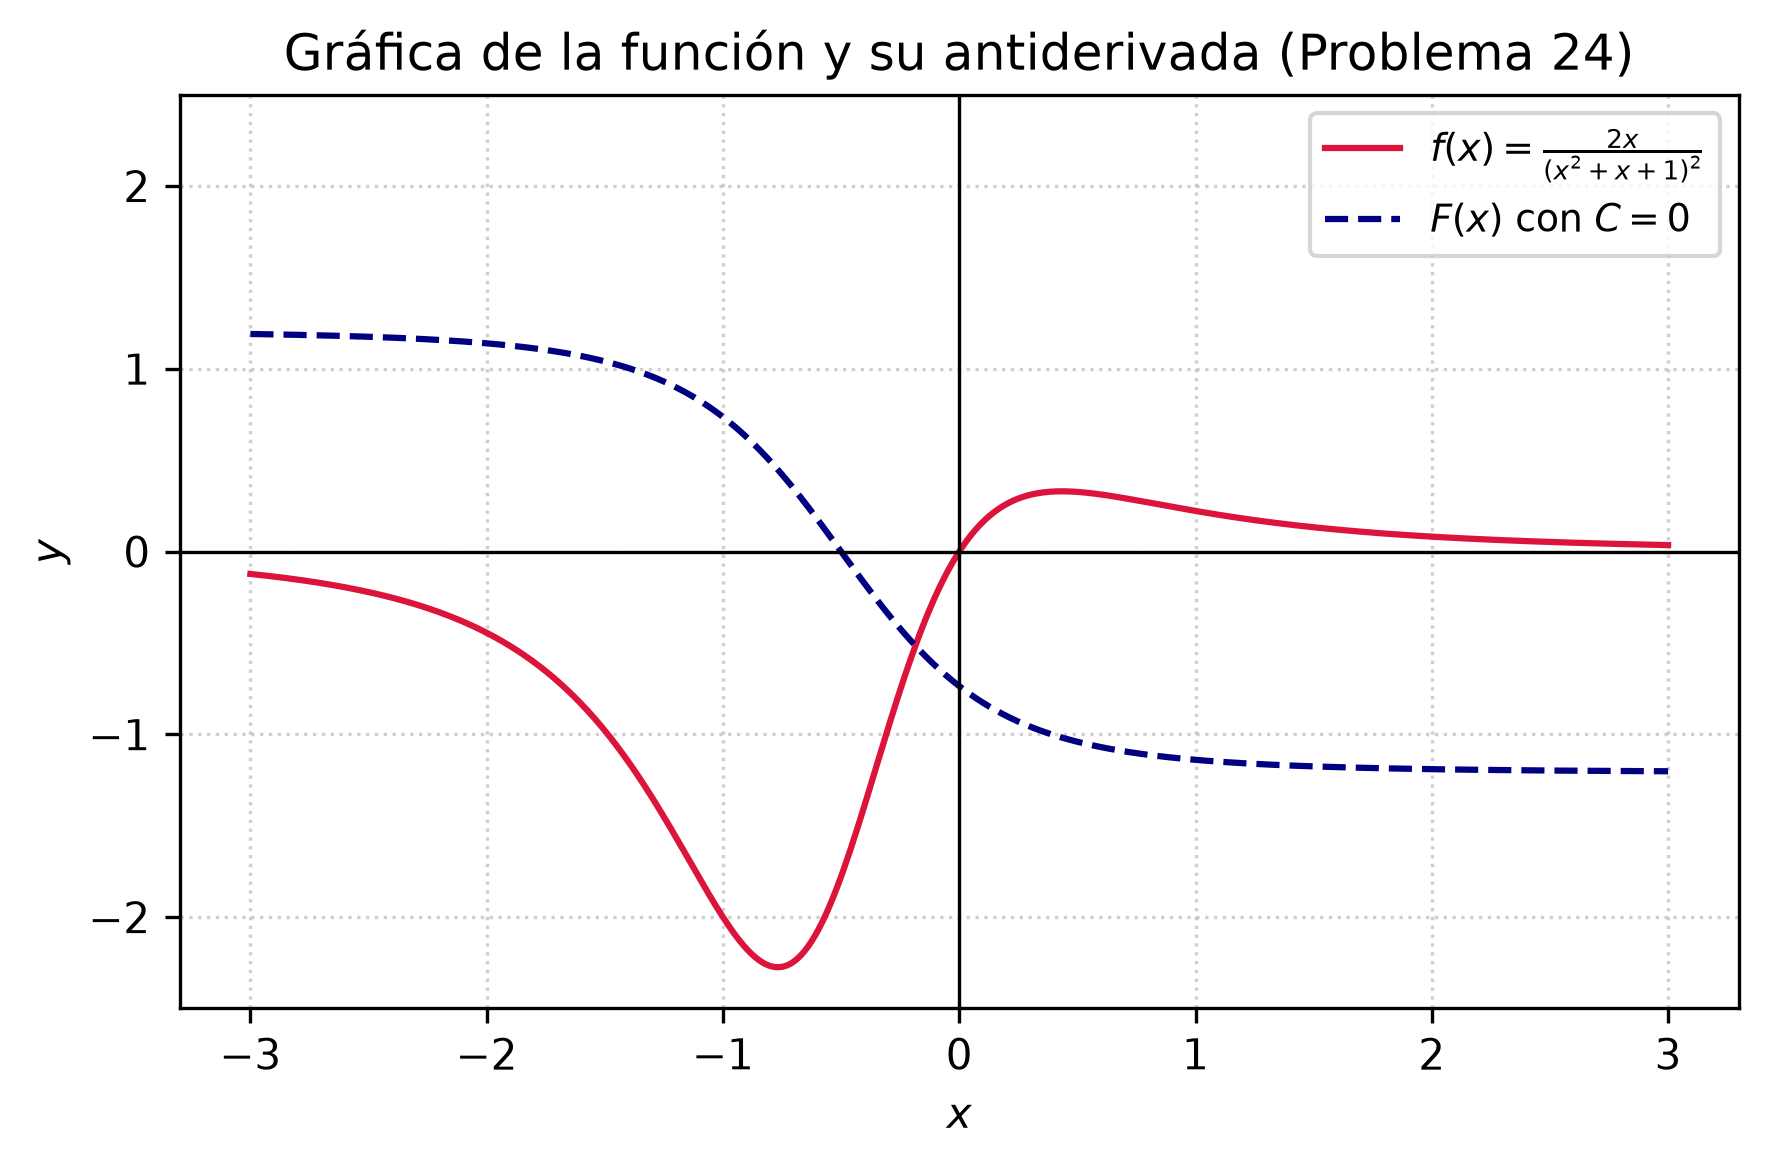
\includegraphics[width=\columnwidth]{semana_03/graficas/SEM03_P24_grafica.png}
	\caption{Representación gráfica de $f(x)$ y su antiderivada $F(x)$ evaluada para la constante de integración $C = 0$ (Problema 24).}
	\label{fig:problema24}
\end{figure}

	\subsection*{Problema 25}

\textbf{Enunciado:} Calcular la integral:
\begin{equation*}
\int \dfrac{x^2 + 2x + 3}{x^3 - x} \, dx
\end{equation*}

\textbf{Solución:} 

Primero, factorizamos el denominador de la función racional. Notamos que:
\begin{equation*}
x^3 - x = x(x^2 - 1) = x(x - 1)(x + 1)
\end{equation*}

Dado que el grado del numerador es menor que el del denominador, aplicamos el método de fracciones parciales:
\begin{multline*}
\dfrac{x^2 + 2x + 3}{x(x - 1)(x + 1)} = \dfrac{A}{x} \\
+ \dfrac{B}{x - 1} + \dfrac{C}{x + 1}
\end{multline*}

Multiplicando toda la ecuación por el denominador común $x(x-1)(x+1)$, obtenemos:
\begin{multline*}
x^2 + 2x + 3 = A(x - 1)(x + 1) \\
+ Bx(x + 1) + Cx(x - 1)
\end{multline*}

Para encontrar los valores de las constantes $A$, $B$ y $C$, evaluamos en valores convenientes de $x$:

Si $x = 0$:
\begin{equation*}
0^2 + 2(0) + 3 = A(0 - 1)(0 + 1)
\end{equation*}
\begin{equation*}
3 = -A \implies A = -3
\end{equation*}

Si $x = 1$:
\begin{equation*}
1^2 + 2(1) + 3 = B(1)(1 + 1)
\end{equation*}
\begin{equation*}
6 = 2B \implies B = 3
\end{equation*}

Si $x = -1$:
\begin{equation*}
(-1)^2 + 2(-1) + 3 = C(-1)(-1 - 1)
\end{equation*}
\begin{equation*}
2 = 2C \implies C = 1
\end{equation*}

Sustituyendo los valores de $A$, $B$ y $C$ en la integral original, tenemos:
\begin{multline*}
\int \dfrac{x^2 + 2x + 3}{x^3 - x} \, dx = \int \left( \dfrac{-3}{x} \right) dx \\
+ \int \dfrac{3}{x - 1} \, dx + \int \dfrac{1}{x + 1} \, dx
\end{multline*}

Integrando cada término por separado, obtenemos la solución general:
\begin{multline*}
\int \dfrac{x^2 + 2x + 3}{x^3 - x} \, dx = -3\ln|x| \\
+ 3\ln|x - 1| + \ln|x + 1| + C
\end{multline*}

Agrupando los logaritmos mediante propiedades, la solución final es:
\begin{equation*}
\ln\left( \dfrac{(x - 1)^3 (x + 1)}{x^3} \right) + C
\end{equation*}

\begin{figure}[H]
	\centering
	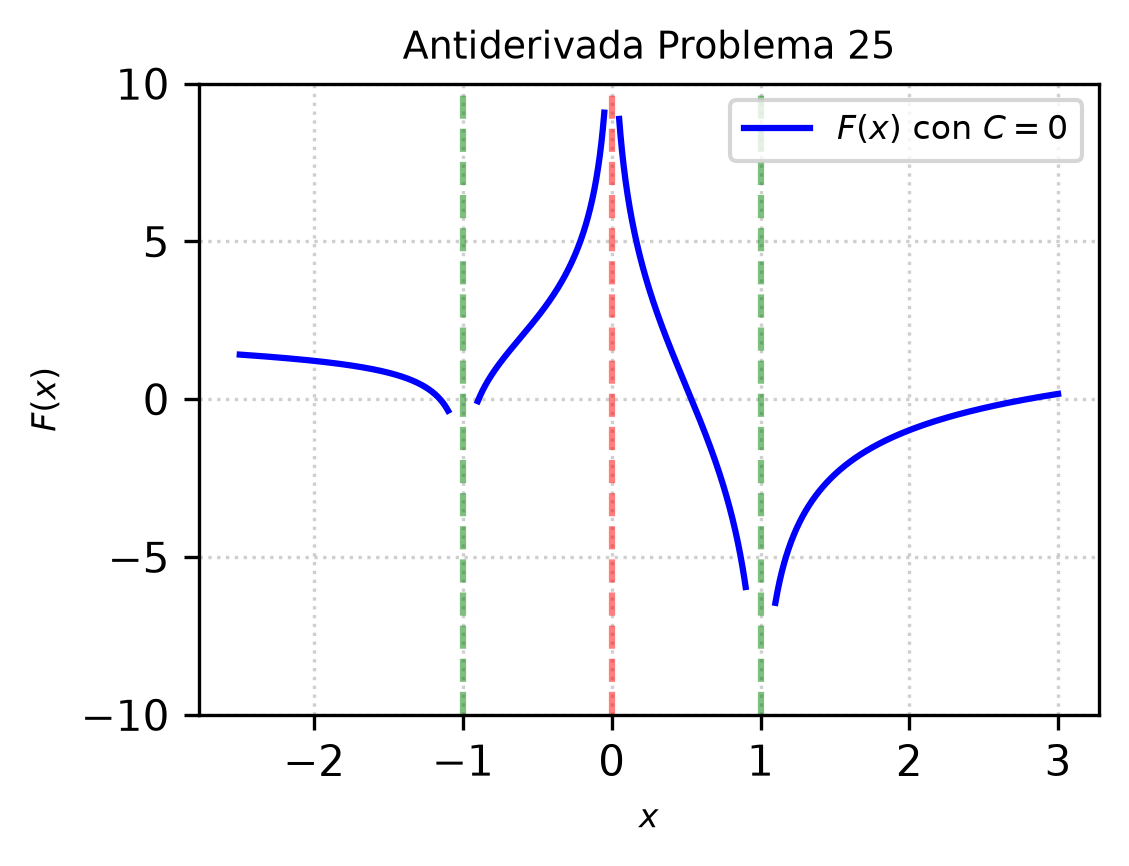
\includegraphics[width=\columnwidth]{semana_03/graficas/SEM03_P25_grafica.png}
	\caption{Representación gráfica de $f(x)$ y su antiderivada $F(x)$ evaluada para la constante de integración $C = 0$ (Problema 25).}
	\label{fig:problema25}
\end{figure}

	\subsection*{Problema 26}

\textbf{Enunciado:}
Calcular la integral indefinida:
\begin{align*}
\int \dfrac{2x^2 - 3x + 5}{(x + 2)(x - 1)(x - 3)} \, dx
\end{align*}

\textbf{Solución:}
El integrando es una función racional propia. Aplicamos el método de fracciones parciales. Suponemos la descomposición:
\begin{align*}
\dfrac{2x^2 - 3x + 5}{(x + 2)(x - 1)(x - 3)} = \dfrac{A}{x + 2} + \dfrac{B}{x - 1} + \dfrac{C}{x - 3}
\end{align*}

Multiplicamos toda la ecuación por el denominador común $(x + 2)(x - 1)(x - 3)$:
\begin{align*}
2x^2 - 3x + 5 &= A(x - 1)(x - 3) \\
&+ B(x + 2)(x - 3) \\
&+ C(x + 2)(x - 1)
\end{align*}

Para hallar las constantes, evaluamos en las raíces del denominador:
Si $x = -2$:
\begin{align*}
2(-2)^2 - 3(-2) + 5 &= A(-3)(-5) \\
8 + 6 + 5 &= 15A \implies 19 = 15A \\
A &= \dfrac{19}{15}
\end{align*}

Si $x = 1$:
\begin{align*}
2(1)^2 - 3(1) + 5 &= B(1 + 2)(1 - 3) \\
2 - 3 + 5 &= B(3)(-2) \\
4 &= -6B \implies B = -\dfrac{2}{3}
\end{align*}

Si $x = 3$:
\begin{align*}
2(3)^2 - 3(3) + 5 &= C(3 + 2)(3 - 1) \\
18 - 9 + 5 &= C(5)(2) \\
14 &= 10C \implies C = \dfrac{7}{5}
\end{align*}

Sustituimos los valores de $A$, $B$ y $C$ en la integral:
\begin{align*}
\int &\left[ \dfrac{19/15}{x + 2} - \dfrac{2/3}{x - 1} + \dfrac{7/5}{x - 3} \right] dx
\end{align*}

Integramos cada término utilizando logaritmos naturales:
\begin{align*}
&= \dfrac{19}{15} \ln|x + 2| - \dfrac{2}{3} \ln|x - 1| \\
&+ \dfrac{7}{5} \ln|x - 3| + C
\end{align*}

\begin{figure}[H]
	\centering
	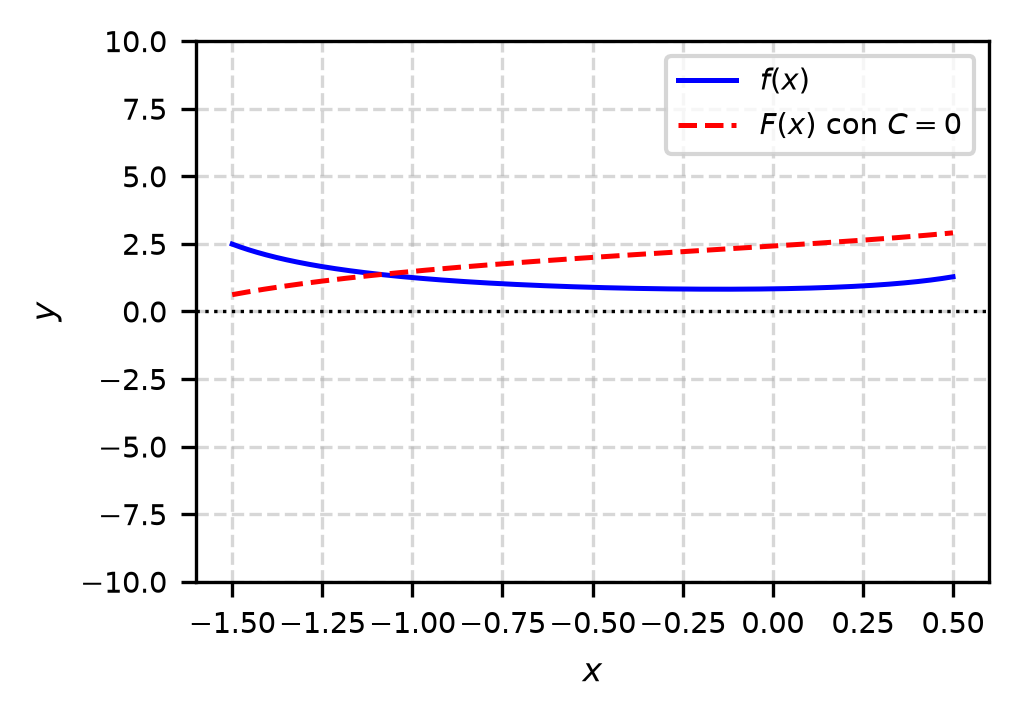
\includegraphics[width=\columnwidth]{semana_03/graficas/SEM03_P26_grafica.png}
	\caption{Representación gráfica de $f(x)$ y su antiderivada $F(x)$ evaluada para la constante de integración $C = 0$ (Problema 26).}
	\label{fig:problema26}
\end{figure}

	\subsection*{Problema 27}

\textbf{Enunciado:}
Calcular la integral indefinida:
\begin{equation*}
\int \dfrac{3x^2 + x - 2}{(x - 1)(x^2 + 1)} \, dx
\end{equation*}

\textbf{Solución:}
Observamos que el integrando es una función racional propia. 
Utilizamos el método de fracciones parciales. 
Planteamos la descomposición:
\begin{align*}
\dfrac{3x^2 + x - 2}{(x - 1)(x^2 + 1)} &= \dfrac{A}{x - 1} \\
&\quad + \dfrac{Bx + C}{x^2 + 1}
\end{align*}

Multiplicando ambos lados por el denominador común $(x - 1)(x^2 + 1)$, obtenemos:
\begin{align*}
3x^2 + x - 2 &= A(x^2 + 1) \\
&\quad + (Bx + C)(x - 1)
\end{align*}

Para hallar los valores de las constantes, evaluamos en valores convenientes de $x$. 
Si $x = 1$:
\begin{align*}
3(1)^2 + 1 - 2 &= A(1^2 + 1) + 0 \\
2 &= 2A \implies A = 1
\end{align*}

Expandimos y agrupamos términos del lado derecho según las potencias de $x$:
\begin{align*}
3x^2 + x - 2 &= Ax^2 + A + Bx^2 \\
&\quad - Bx + Cx - C \\
&= (A + B)x^2 \\
&\quad + (C - B)x + (A - C)
\end{align*}

Igualando los coeficientes de ambos lados:
\begin{align*}
A + B &= 3 \\
C - B &= 1 \\
A - C &= -2
\end{align*}

Como $A = 1$, de la primera ecuación:
\begin{align*}
1 + B &= 3 \implies B = 2
\end{align*}

De la tercera ecuación:
\begin{align*}
1 - C &= -2 \implies C = 3
\end{align*}

Sustituyendo las constantes $A$, $B$ y $C$ en la descomposición original:
\begin{align*}
\int &\dfrac{3x^2 + x - 2}{(x - 1)(x^2 + 1)} \, dx = \\
&\int \left( \dfrac{1}{x - 1} + \dfrac{2x + 3}{x^2 + 1} \right) dx
\end{align*}

Separamos la integral en tres partes para facilitar la integración directa:
\begin{align*}
&= \int \dfrac{1}{x - 1} \, dx \\
&\quad + \int \dfrac{2x}{x^2 + 1} \, dx + \int \dfrac{3}{x^2 + 1} \, dx
\end{align*}

Integramos cada término aplicando fórmulas estándar (logaritmo natural y arcotangente):
\begin{align*}
&= \ln|x - 1| + \ln(x^2 + 1) \\
&\quad + 3\arctan(x) + C
\end{align*}

Por lo tanto, la solución general de la integral es:
\begin{equation*}
\ln|x - 1| + \ln(x^2 + 1) + 3\arctan(x) + C
\end{equation*}

\begin{figure}[H]
	\centering
	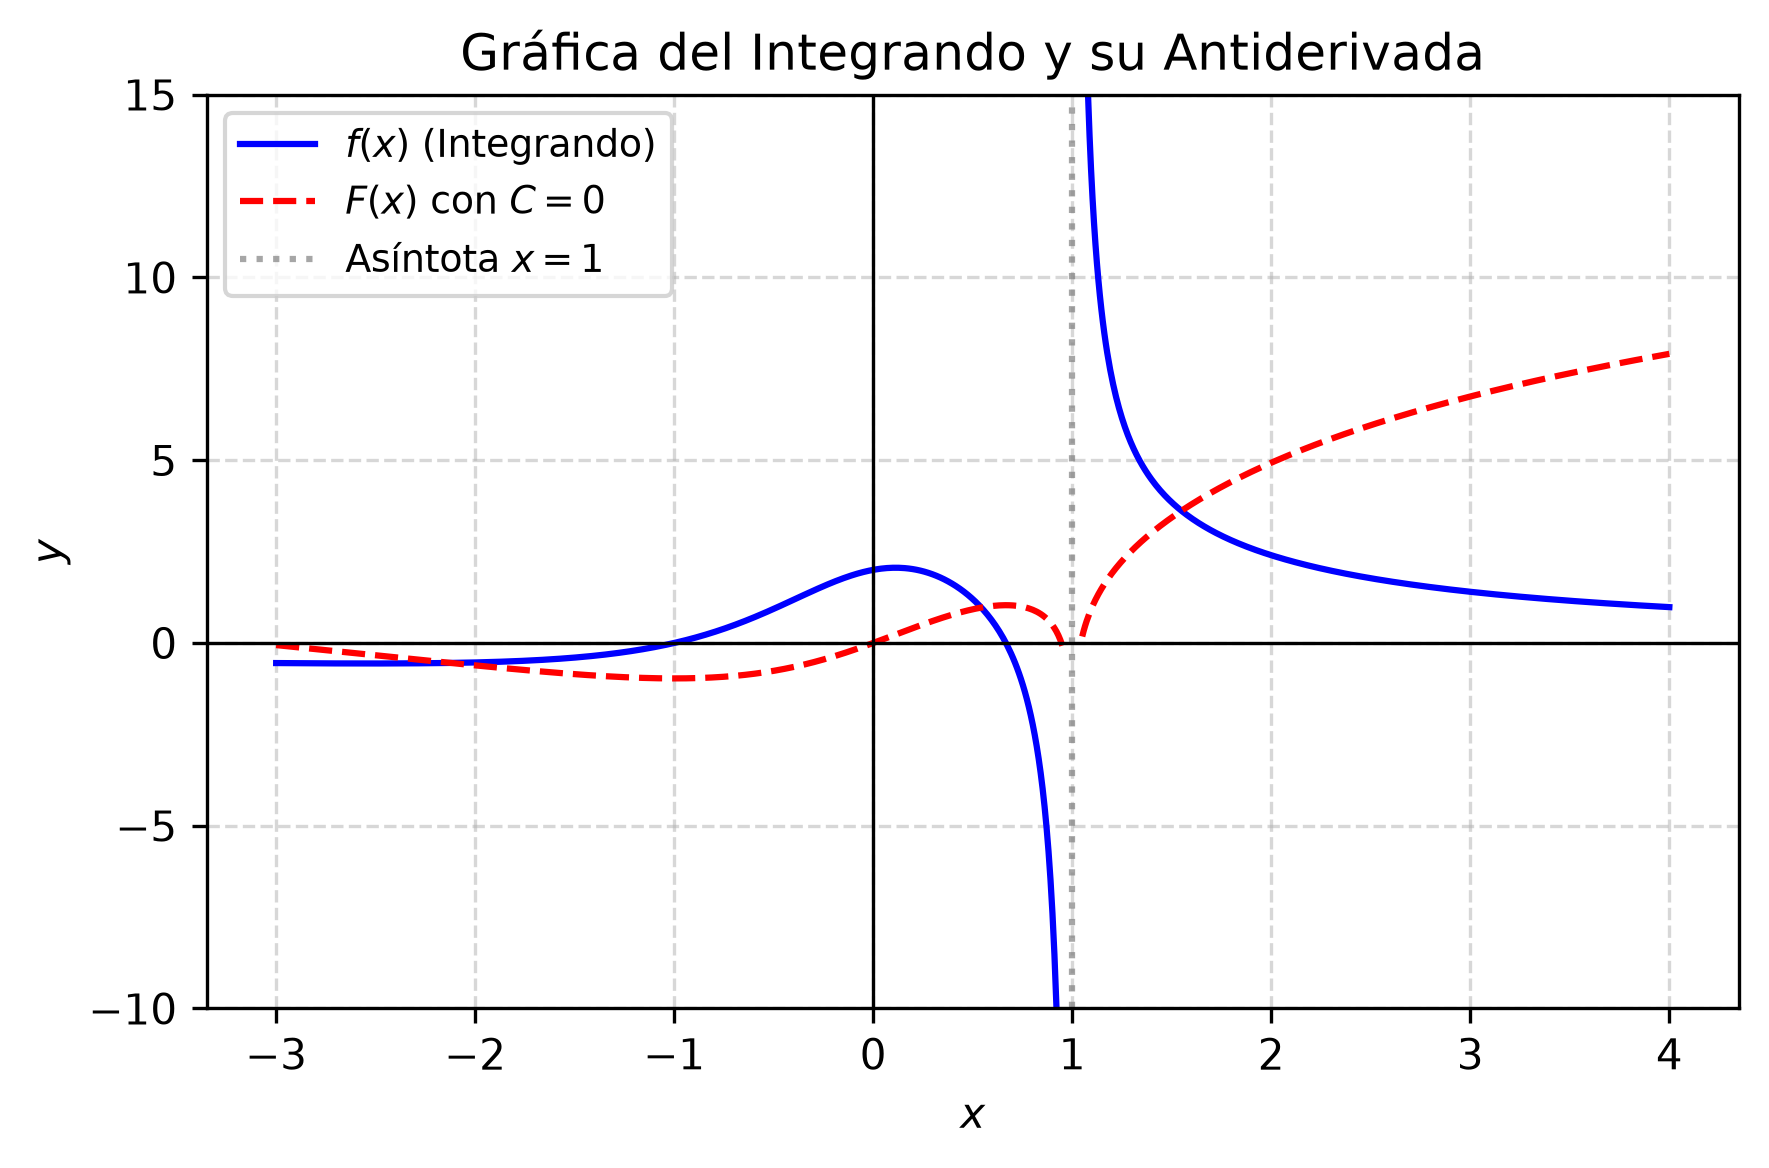
\includegraphics[width=\columnwidth]{semana_03/graficas/SEM03_P27_grafica.png}
	\caption{Representación gráfica de $f(x)$ y su antiderivada $F(x)$ evaluada para la constante de integración $C = 0$ (Problema 27).}
	\label{fig:problema27}
\end{figure}

	\subsection*{Problema 28}

\textbf{Enunciado:} Calcular la integral:
\begin{equation*}
\int \dfrac{x + 5}{x^3 - 3x + 2} \, dx
\end{equation*}

\textbf{Solución:} 
Primero, factorizamos el denominador 
$P(x) = x^3 - 3x + 2$. 
Dado que $x = 1$ es una raíz evidente 
($1^3 - 3(1) + 2 = 0$), 
utilizamos división sintética o factorización 
por polinomios para obtener:
\begin{equation*}
x^3 - 3x + 2 = (x - 1)^2 (x + 2)
\end{equation*}

Planteamos la descomposición en 
fracciones parciales con factores 
repetidos y lineales:
\begin{multline*}
\dfrac{x + 5}{(x - 1)^2 (x + 2)} = \\
\dfrac{A}{x - 1} + \dfrac{B}{(x - 1)^2} + \dfrac{C}{x + 2}
\end{multline*}

Multiplicando ambos lados por el 
denominador común, obtenemos:
\begin{multline*}
x + 5 = A(x - 1)(x + 2) \\
+ B(x + 2) + C(x - 1)^2
\end{multline*}

Evaluamos en los valores clave para 
encontrar las constantes:
Si $x = 1$:
\begin{align*}
1 + 5 &= B(1 + 2) \implies 6 = 3B \implies B = 2
\end{align*}

Si $x = -2$:
\begin{align*}
-2 + 5 &= C(-2 - 1)^2 \implies 3 = 9C \implies C = \dfrac{1}{3}
\end{align*}

Si $x = 0$ y usando $B = 2$, $C = \dfrac{1}{3}$:
\begin{align*}
5 &= A(-1)(2) + 2(2) + \dfrac{1}{3}(-1)^2 \\
5 &= -2A + 4 + \dfrac{1}{3} \implies 2A = \dfrac{4}{3} \implies A = \dfrac{2}{3}
\end{align*}

Reemplazando los valores en la integral:
\begin{multline*}
\int \dfrac{x + 5}{x^3 - 3x + 2} \, dx = 
\int \left( \dfrac{2/3}{x - 1} + \dfrac{2}{(x - 1)^2} \right. \\
\left. + \dfrac{1/3}{x + 2} \right) dx
\end{multline*}

Integrando término a término:
\begin{align*}
&= \dfrac{2}{3}\ln|x - 1| - \dfrac{2}{x - 1} + \dfrac{1}{3}\ln|x + 2| + C
\end{align*}

Agrupando los términos logarítmicos:
\begin{align*}
&= \dfrac{1}{3}\ln\left| \dfrac{(x - 1)^2(x + 2)}{(x - 1)^3} \right| - \dfrac{2}{x - 1} + C
\end{align*}

La solución general de la integral es:
\begin{equation*}
\int \dfrac{x + 5}{x^3 - 3x + 2} \, dx = 
\dfrac{1}{3}\ln\left| \dfrac{x + 2}{x - 1} \right| - \dfrac{2}{x - 1} + C
\end{equation*}

\begin{figure}[H]
	\centering
	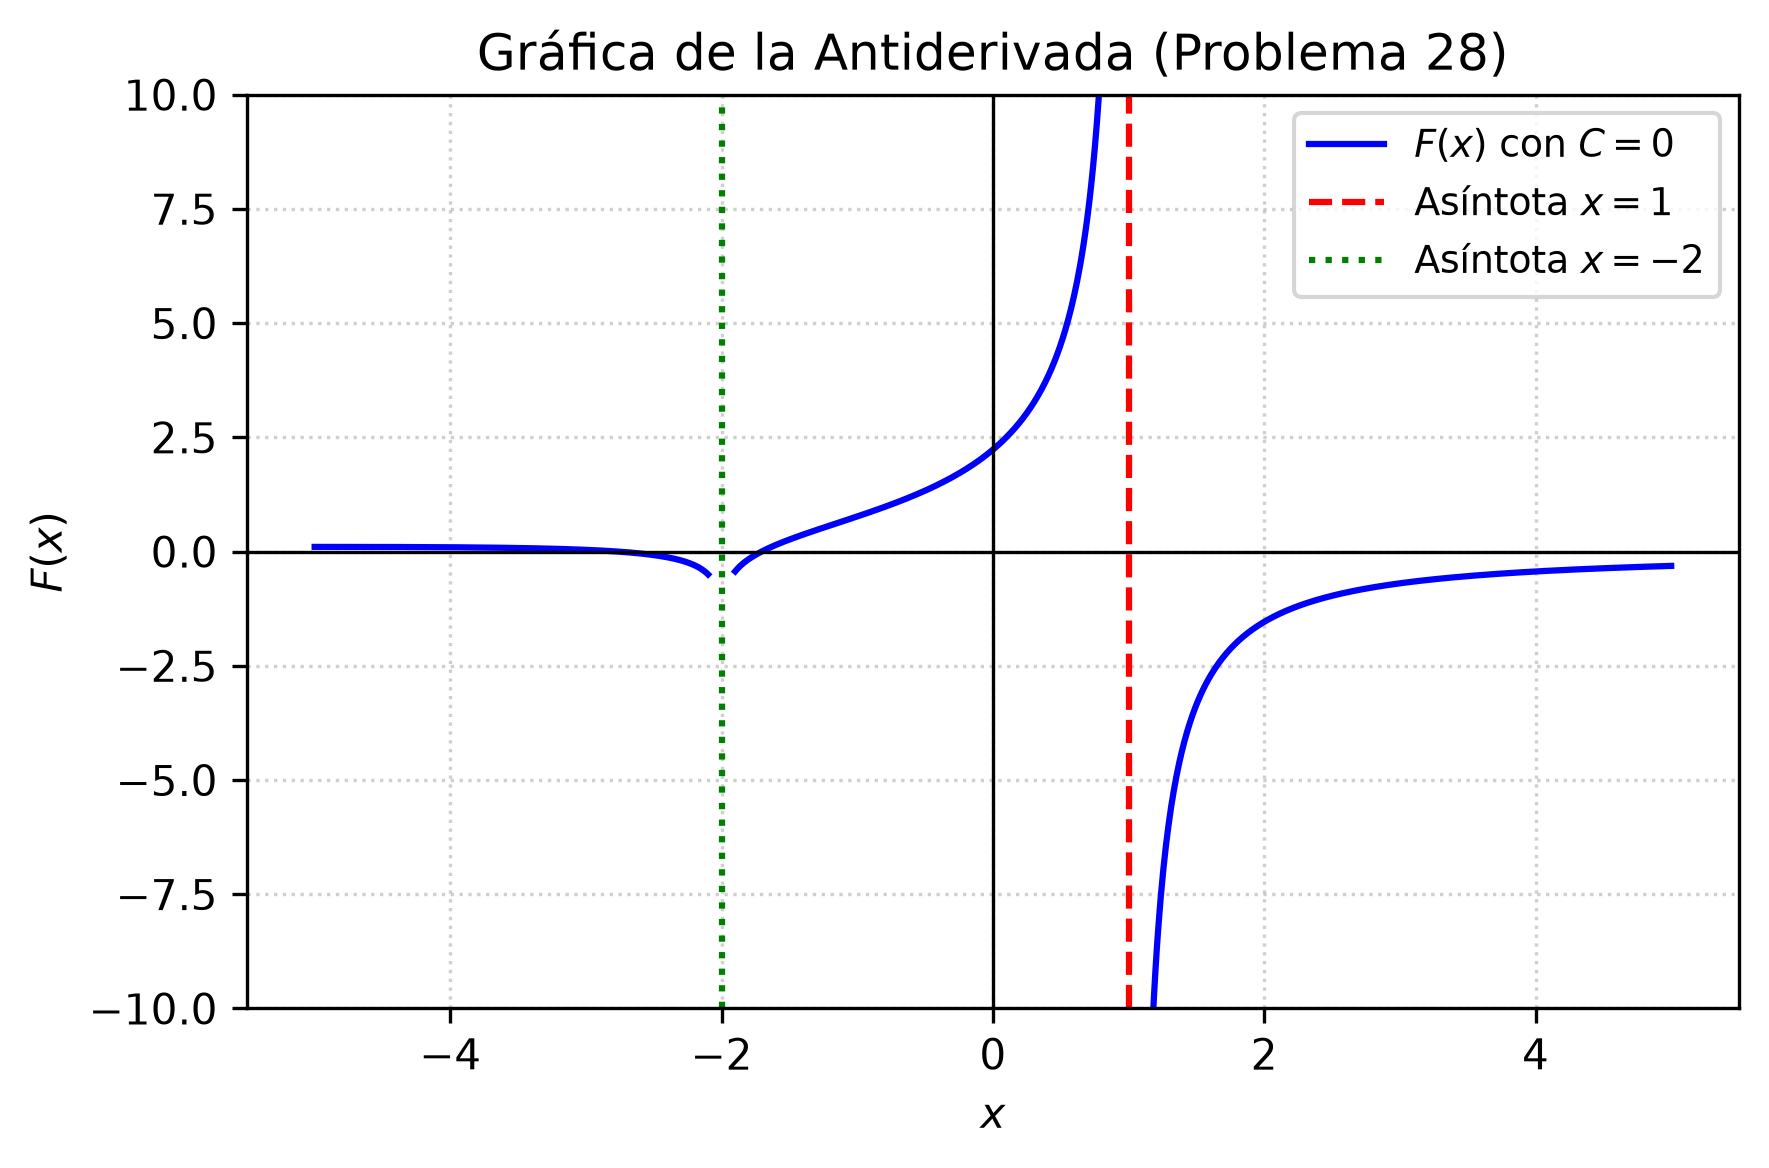
\includegraphics[width=\columnwidth]{semana_03/graficas/SEM03_P28_grafica.png}
	\caption{Representación gráfica de $f(x)$ y su antiderivada $F(x)$ evaluada para la constante de integración $C = 0$ (Problema 28).}
	\label{fig:problema28}
\end{figure}

	\subsection*{Problema 29}
\textbf{Enunciado:} Calcular la integral:
\begin{align*}
\int \dfrac{2x^3 + 3x^2 + x - 1}{(x + 1)(x^2 + 2x + 2)^2} \, dx
\end{align*}

\textbf{Solución:} 
El integrando es una función racional propia. 
Utilizamos el método de fracciones parciales:
\begin{align*}
\dfrac{2x^3 + 3x^2 + x - 1}{(x + 1)(x^2 + 2x + 2)^2} = \dfrac{A}{x + 1} \\
+ \dfrac{Bx + C}{x^2 + 2x + 2} + \dfrac{Dx + E}{(x^2 + 2x + 2)^2}
\end{align*}

Multiplicando por el denominador común e igualando numeradores, evaluando en $x = -1$ obtenemos $A = 1$. 
Para los demás coeficientes, expandimos y agrupamos términos semejantes, resultando en:
$B = 1$, $C = 0$, $D = 1$ y $E = 1$. 
Sustituyendo los valores:
\begin{align*}
\int \left( \dfrac{1}{x + 1} + \dfrac{x}{x^2 + 2x + 2} \right. \\
\left. + \dfrac{x + 1}{(x^2 + 2x + 2)^2} \right) dx
\end{align*}

Integramos cada término por separado. 
Para el segundo término, completamos el diferencial del denominador:
\begin{align*}
\int \dfrac{x}{x^2 + 2x + 2} \, dx = \dfrac{1}{2}\ln(x^2 + 2x + 2) \\
- \arctan(x + 1)
\end{align*}

Para el tercer término, usamos la sustitución trigonométrica sugerida $x + 1 = \tan(\theta)$:
\begin{align*}
\int \dfrac{x + 1}{((x + 1)^2 + 1)^2} \, dx = -\dfrac{1}{2(x^2 + 2x + 2)}
\end{align*}

Combinando todos los resultados y añadiendo la constante de integración $C$, obtenemos la solución general:
\begin{align*}
I = \ln|x + 1| + \dfrac{1}{2}\ln(x^2 + 2x + 2) \\
- \arctan(x + 1) - \dfrac{1}{2(x^2 + 2x + 2)} + C
\end{align*}

\begin{figure}[H]
	\centering
	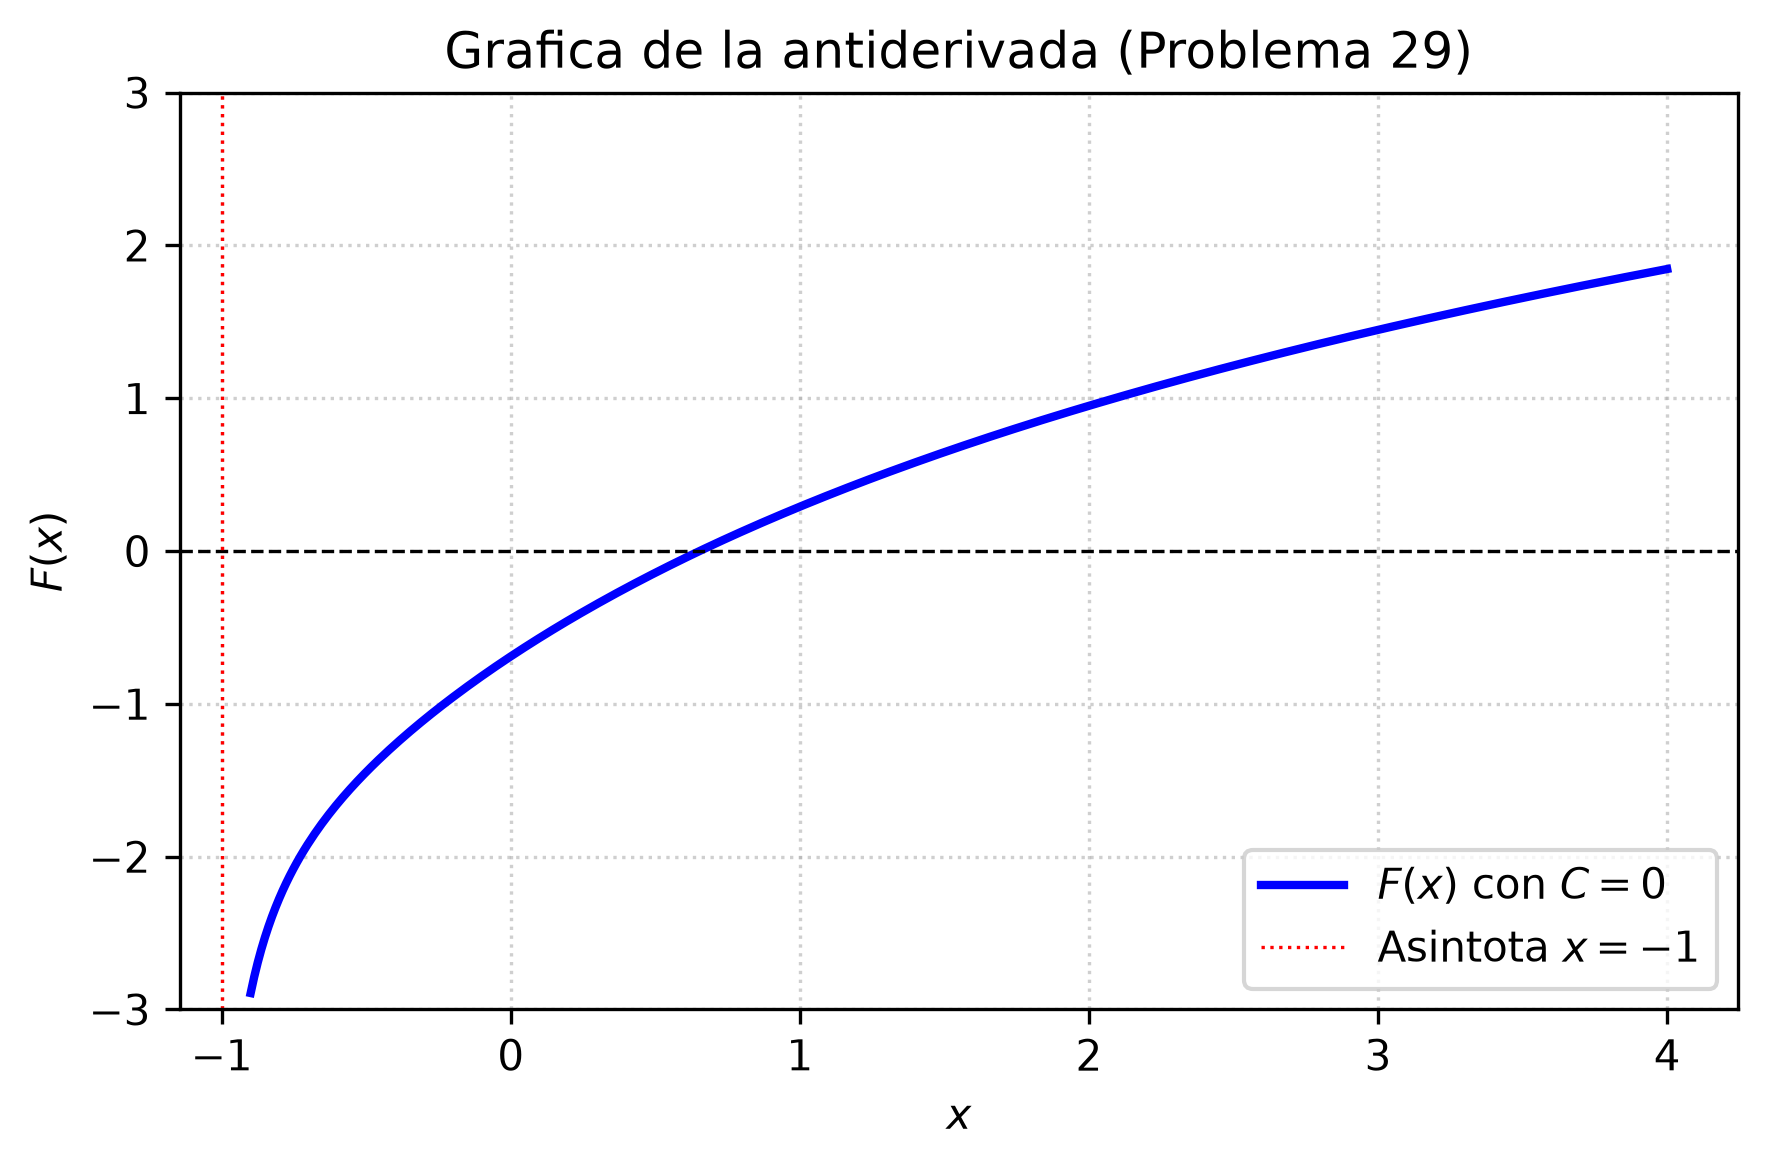
\includegraphics[width=\columnwidth]{semana_03/graficas/SEM03_P29_grafica.png}
	\caption{Representación gráfica de $f(x)$ y su antiderivada $F(x)$ evaluada para la constante de integración $C = 0$ (Problema 29).}
	\label{fig:problema29}
\end{figure}

	\subsection*{Problema 30}
\textbf{Enunciado:} Calcular la integral:
\begin{align*}
\int \dfrac{2x + 1}{3x^3 + 2x - 1} \, dx
\end{align*}

\textbf{Solución:} 
Utilizamos el método de descomposición en fracciones parciales. 
Primero, encontramos las raíces del polinomio denominador:
\begin{align*}
P(x) = 3x^3 + 2x - 1
\end{align*}
Probando con la raíz racional $x = \dfrac{1}{3}$, tenemos:
\begin{align*}
P\left(\dfrac{1}{3}\right) = 3\left(\dfrac{1}{27}\right) + 2\left(\dfrac{1}{3}\right) - 1 = 0
\end{align*}
Por lo tanto, $(3x - 1)$ es un factor del polinomio. Al dividir $P(x)$ entre $(3x - 1)$ mediante división sintética o polinómica, obtenemos el trinomio cuadrático:
\begin{align*}
3x^3 + 2x - 1 = (3x - 1)(x^2 + \dfrac{1}{3}x + 1)
\end{align*}
Para evitar fracciones complejas, multiplicamos y dividimos por $3$ dentro del trinomio:
\begin{align*}
3x^3 + 2x - 1 = (3x - 1)(x^2 + \dfrac{1}{3}x + 1)
\end{align*}

Planteamos la descomposición en fracciones parciales de la forma:
\begin{align*}
\dfrac{2x + 1}{3x^3 + 2x - 1} = \dfrac{A}{3x - 1} + \dfrac{Bx + C}{x^2 + \dfrac{x}{3} + 1}
\end{align*}

Multiplicando ambos lados por el denominador común:
\begin{align*}
2x + 1 = &A\left(x^2 + \dfrac{x}{3} + 1\right) \\
&+ (Bx + C)(3x - 1)
\end{align*}

Evaluando en $x = \dfrac{1}{3}$:
\begin{align*}
2\left(\dfrac{1}{3}\right) + 1 &= A\left(\left(\dfrac{1}{3}\right)^2 + \dfrac{1}{9} + 1\right) \\
\dfrac{5}{3} &= A\left(\dfrac{1}{9} + \dfrac{1}{9} + 1\right) = \dfrac{11}{9}A
\end{align*}
De donde obtenemos $A = \dfrac{15}{11}$.

Igualando coeficientes para las potencias de $x^2$:
\begin{align*}
0 &= A + 3B \implies B = -\dfrac{A}{3} = -\dfrac{5}{11}
\end{align*}

Igualando los términos independientes ($x^0$):
\begin{align*}
1 &= A - C \implies C = A - 1 \\
C &= \dfrac{15}{11} - 1 = \dfrac{4}{11}
\end{align*}

Sustituyendo los valores de $A$, $B$ y $C$ en la integral:
\begin{align*}
\int &\dfrac{2x + 1}{3x^3 + 2x - 1} \, dx = \\
&\int \left( \dfrac{\frac{15}{11}}{3x - 1} + \dfrac{-\frac{5}{11}x + \frac{4}{11}}{x^2 + \frac{x}{3} + 1} \right) dx
\end{align*}

La primera integral es inmediata:
\begin{align*}
\int \dfrac{\frac{15}{11}}{3x - 1} \, dx = \dfrac{5}{11} \ln|3x - 1|
\end{align*}

Para la segunda integral, completamos el binomio en el denominador:
\begin{align*}
x^2 + \dfrac{x}{3} + 1 = \left(x + \dfrac{1}{6}\right)^2 + \dfrac{35}{36}
\end{align*}
Y ajustamos el numerador para que aparezca la derivada del denominador ($2x + \dfrac{1}{3}$):
\begin{align*}
-\dfrac{5}{11}x + \dfrac{4}{11} = -\dfrac{5}{22}\left(2x + \dfrac{1}{3}\right) + \dfrac{55}{132}
\end{align*}

Integrando esta parte obtenemos un término logarítmico y uno de arco tangente:
\begin{align*}
-\dfrac{5}{22} &\ln\left(x^2 + \dfrac{x}{3} + 1\right) \\
&+ \dfrac{9}{2\sqrt{35}} \arctan\left(\dfrac{6x + 1}{\sqrt{35}}\right)
\end{align*}

Combinando todos los resultados, la solución general es:
\begin{align*}
F(x) &= \dfrac{5}{11} \ln|3x - 1| \\
&- \dfrac{5}{22} \ln\left(x^2 + \dfrac{x}{3} + 1\right) \\
&+ \dfrac{9}{2\sqrt{35}} \arctan\left(\dfrac{6x + 1}{\sqrt{35}}\right) + C
\end{align*}

\begin{figure}[H]
	\centering
	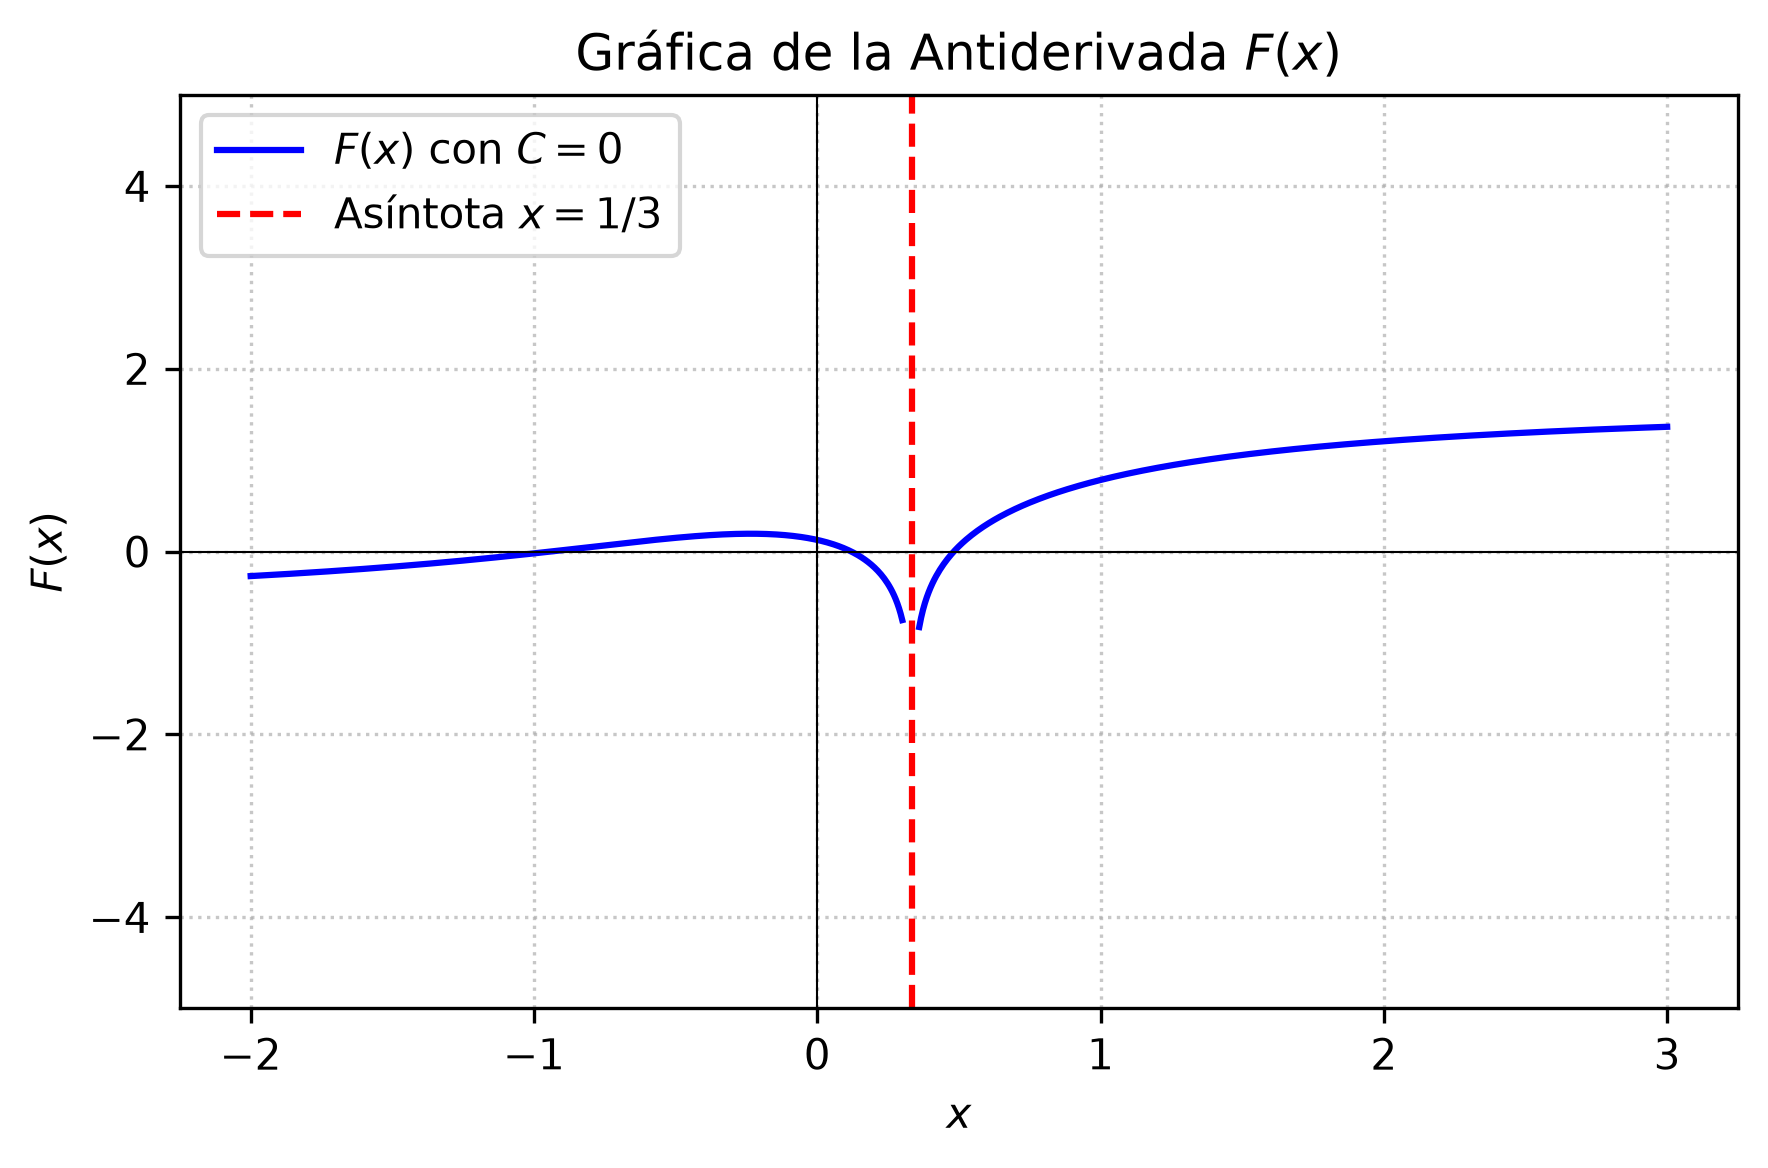
\includegraphics[width=\columnwidth]{semana_03/graficas/SEM03_P30_grafica.png}
	\caption{Representación gráfica de $f(x)$ y su antiderivada $F(x)$ evaluada para la constante de integración $C = 0$ (Problema 30).}
	\label{fig:problema30}
\end{figure}

	\subsection*{Problema 31}
\textbf{Enunciado:} Calcular la integral:
\begin{align*}
\int \dfrac{2x^2 + 3x - 1}{x^3 + 2x^2 + 4x + 2} \, dx
\end{align*}

\textbf{Solución:}
Primero, analizamos el denominador 
$P(x) = x^3 + 2x^2 + 4x + 2$. 
Buscamos raíces racionales usando los divisores del término constante ($2$), los cuales son $\pm 1, \pm 2$. Evaluando en $x = -1$:
\begin{align*}
P(-1) &= (-1)^3 + 2(-1)^2 + 4(-1) + 2 \\
&= -1 + 2 - 4 + 2 = -1 \neq 0
\end{align*}
Probamos agrupando términos o usando división sintética. Notemos que si factorizamos por división:
\begin{align*}
x^3 + 2x^2 + 4x + 2 = (x+1)(x^2 + x + 2)
\end{align*}
El trinomio $x^2 + x + 2$ tiene un discriminante negativo ($\Delta = 1^2 - 4(1)(2) = -7$), por lo que es irreducible en los reales.

Planteamos la descomposición en fracciones parciales de la siguiente manera:
\begin{align*}
\dfrac{2x^2 + 3x - 1}{(x+1)(x^2 + x + 2)} &= \dfrac{A}{x+1} \\
&+ \dfrac{Bx + C}{x^2 + x + 2}
\end{align*}

Multiplicando toda la expresión por el denominador común, obtenemos:
\begin{align*}
2x^2 + 3x - 1 &= A(x^2 + x + 2) \\
&+ (Bx + C)(x+1)
\end{align*}

Evaluamos en $x = -1$ para hallar $A$:
\begin{align*}
2(-1)^2 + 3(-1) - 1 &= A((-1)^2 + (-1) + 2) \\
2 - 3 - 1 &= A(1 - 1 + 2) \\
-2 &= 2A \implies A = -1
\end{align*}

Expandimos y agrupamos términos para $B$ y $C$:
\begin{align*}
2x^2 + 3x - 1 &= Ax^2 + Ax + 2A \\
&+ Bx^2 + Bx + Cx + C \\
&= (A+B)x^2 + (A+B+C)x \\
&+ (2A+C)
\end{align*}

Igualando coeficientes:
\begin{align*}
A + B &= 2 \implies -1 + B = 2 \implies B = 3 \\
2A + C &= -1 \implies 2(-1) + C = -1 \implies C = 1
\end{align*}

Sustituimos los valores hallados en la integral original:
\begin{align*}
\int &\left( \dfrac{-1}{x+1} + \dfrac{3x + 1}{x^2 + x + 2} \right) dx
\end{align*}

Integramos el primer término directamente:
\begin{align*}
\int \dfrac{-1}{x+1} \, dx = -\ln|x+1|
\end{align*}

Para el segundo término, derivamos el denominador: $\frac{d}{dx}(x^2+x+2) = 2x+1$. Ajustamos el numerador:
\begin{align*}
\dfrac{3x+1}{x^2+x+2} &= \dfrac{\frac{3}{2}(2x+1) - \frac{3}{2} + 1}{x^2+x+2} \\
&= \dfrac{\frac{3}{2}(2x+1) - \frac{1}{2}}{x^2+x+2}
\end{align*}

Separamos en dos integrales:
\begin{align*}
\int \dfrac{\frac{3}{2}(2x+1)}{x^2+x+2} \, dx &= \dfrac{3}{2}\ln|x^2+x+2| \\
\int \dfrac{-\frac{1}{2}}{(x+\frac{1}{2})^2 + \frac{7}{4}} \, dx &= -\dfrac{1}{2} \cdot \dfrac{2}{\sqrt{7}}\arctan\left(\frac{x+\frac{1}{2}}{\frac{\sqrt{7}}{2}}\right)
\end{align*}

Uniendo todos los resultados y agregando la constante de integración $C$:
\begin{align*}
F(x) &= -\ln|x+1| + \dfrac{3}{2}\ln(x^2+x+2) \\
&- \dfrac{1}{\sqrt{7}}\arctan\left(\frac{2x+1}{\sqrt{7}}\right) + C
\end{align*}

\begin{figure}[H]
	\centering
	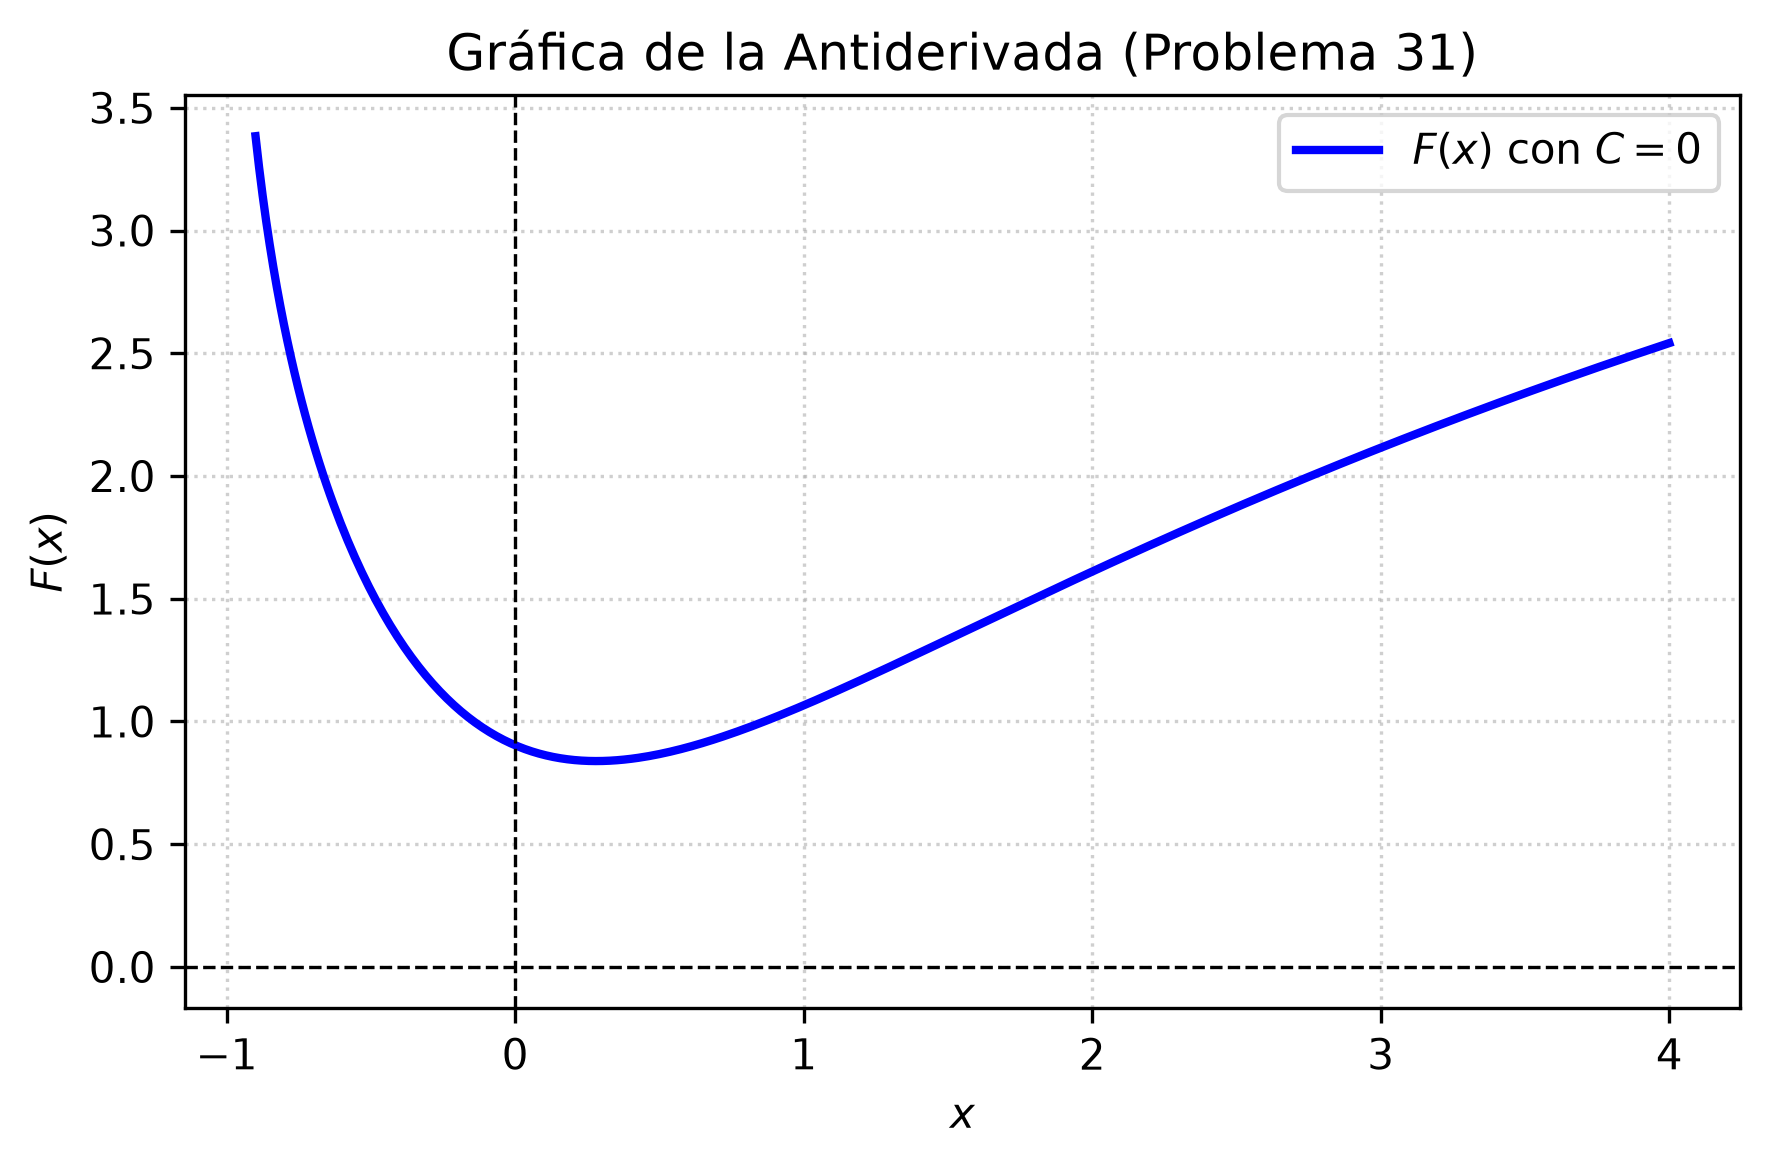
\includegraphics[width=\columnwidth]{semana_03/graficas/SEM03_P31_grafica.png}
	\caption{Representación gráfica de $f(x)$ y su antiderivada $F(x)$ evaluada para la constante de integración $C = 0$ (Problema 31).}
	\label{fig:problema31}
\end{figure}

	\subsection*{Problema 32}

\textbf{Enunciado:} Calcular la integral:
\begin{align*}
\int \dfrac{x^4 - 2x^2 + 3x + 4}{(x - 1)^3 (x^2 + 2x + 2)} \, dx
\end{align*}

\textbf{Solución:} 
El integrando es una función racional propia. 
Utilizamos el método de fracciones parciales 
con factores lineales repetidos y cuadráticos 
irreducibles:
\begin{align*}
\dfrac{x^4 - 2x^2 + 3x + 4}{(x - 1)^3 (x^2 + 2x + 2)} = 
&\dfrac{A}{x - 1} + \dfrac{B}{(x - 1)^2} \\
&+ \dfrac{C}{(x - 1)^3} + \dfrac{Dx + E}{x^2 + 2x + 2}
\end{align*}

Multiplicando ambos lados por el denominador común:
\begin{align*}
x^4 - 2x^2 + 3x + 4 = 
&A(x - 1)^2(x^2 + 2x + 2) \\
&+ B(x - 1)(x^2 + 2x + 2) \\
&+ C(x^2 + 2x + 2) \\
&+ (Dx + E)(x - 1)^3
\end{align*}

Evaluando en $x = 1$:
\begin{align*}
1^4 - 2(1)^2 + 3(1) + 4 &= C(1^2 + 2(1) + 2) \\
6 &= 5C \implies C = \dfrac{6}{5}
\end{align*}

Desarrollando y agrupando coeficientes por potencias de $x$, 
o aplicando derivadas sucesivas para $A$, $B$, $D$ y $E$:
\begin{align*}
A &= -\dfrac{1}{25}, \quad B = \dfrac{17}{5}, \quad C = \dfrac{6}{5}, \\
D &= \dfrac{26}{25}, \quad E = -\dfrac{38}{25}
\end{align*}

Sustituyendo las fracciones parciales e integrando 
término a término:
\begin{align*}
\int &\left( \dfrac{-1/25}{x - 1} + \dfrac{17/5}{(x - 1)^2} + \dfrac{6/5}{(x - 1)^3} \right) dx \\
&+ \int \dfrac{\frac{26}{25}x - \frac{38}{25}}{x^2 + 2x + 2} \, dx
\end{align*}

Resolviendo las tres primeras integrales directas:
\begin{align*}
-\dfrac{1}{25}\ln|x - 1| - \dfrac{17}{5(x - 1)} - \dfrac{3}{5(x - 1)^2}
\end{align*}

Para la integral restante, completamos el trinomio 
en el denominador $x^2 + 2x + 2 = (x + 1)^2 + 1$ 
y ajustamos el numerador:
\begin{align*}
\int \dfrac{\frac{26}{25}x - \frac{38}{25}}{(x + 1)^2 + 1} \, dx = 
\dfrac{13}{25}\ln(x^2 + 2x + 2) \\
- \dfrac{51}{25}\arctan(x + 1)
\end{align*}

Finalmente, unimos todos los resultados y 
agregamos la constante de integración $C_{int}$:
\begin{align*}
F(x) &= -\dfrac{1}{25}\ln|x - 1| + \dfrac{13}{25}\ln(x^2 + 2x + 2) \\
&\quad - \dfrac{17}{5(x - 1)} - \dfrac{3}{5(x - 1)^2} \\
&\quad - \dfrac{51}{25}\arctan(x + 1) + C_{int}
\end{align*}

\begin{figure}[H]
	\centering
	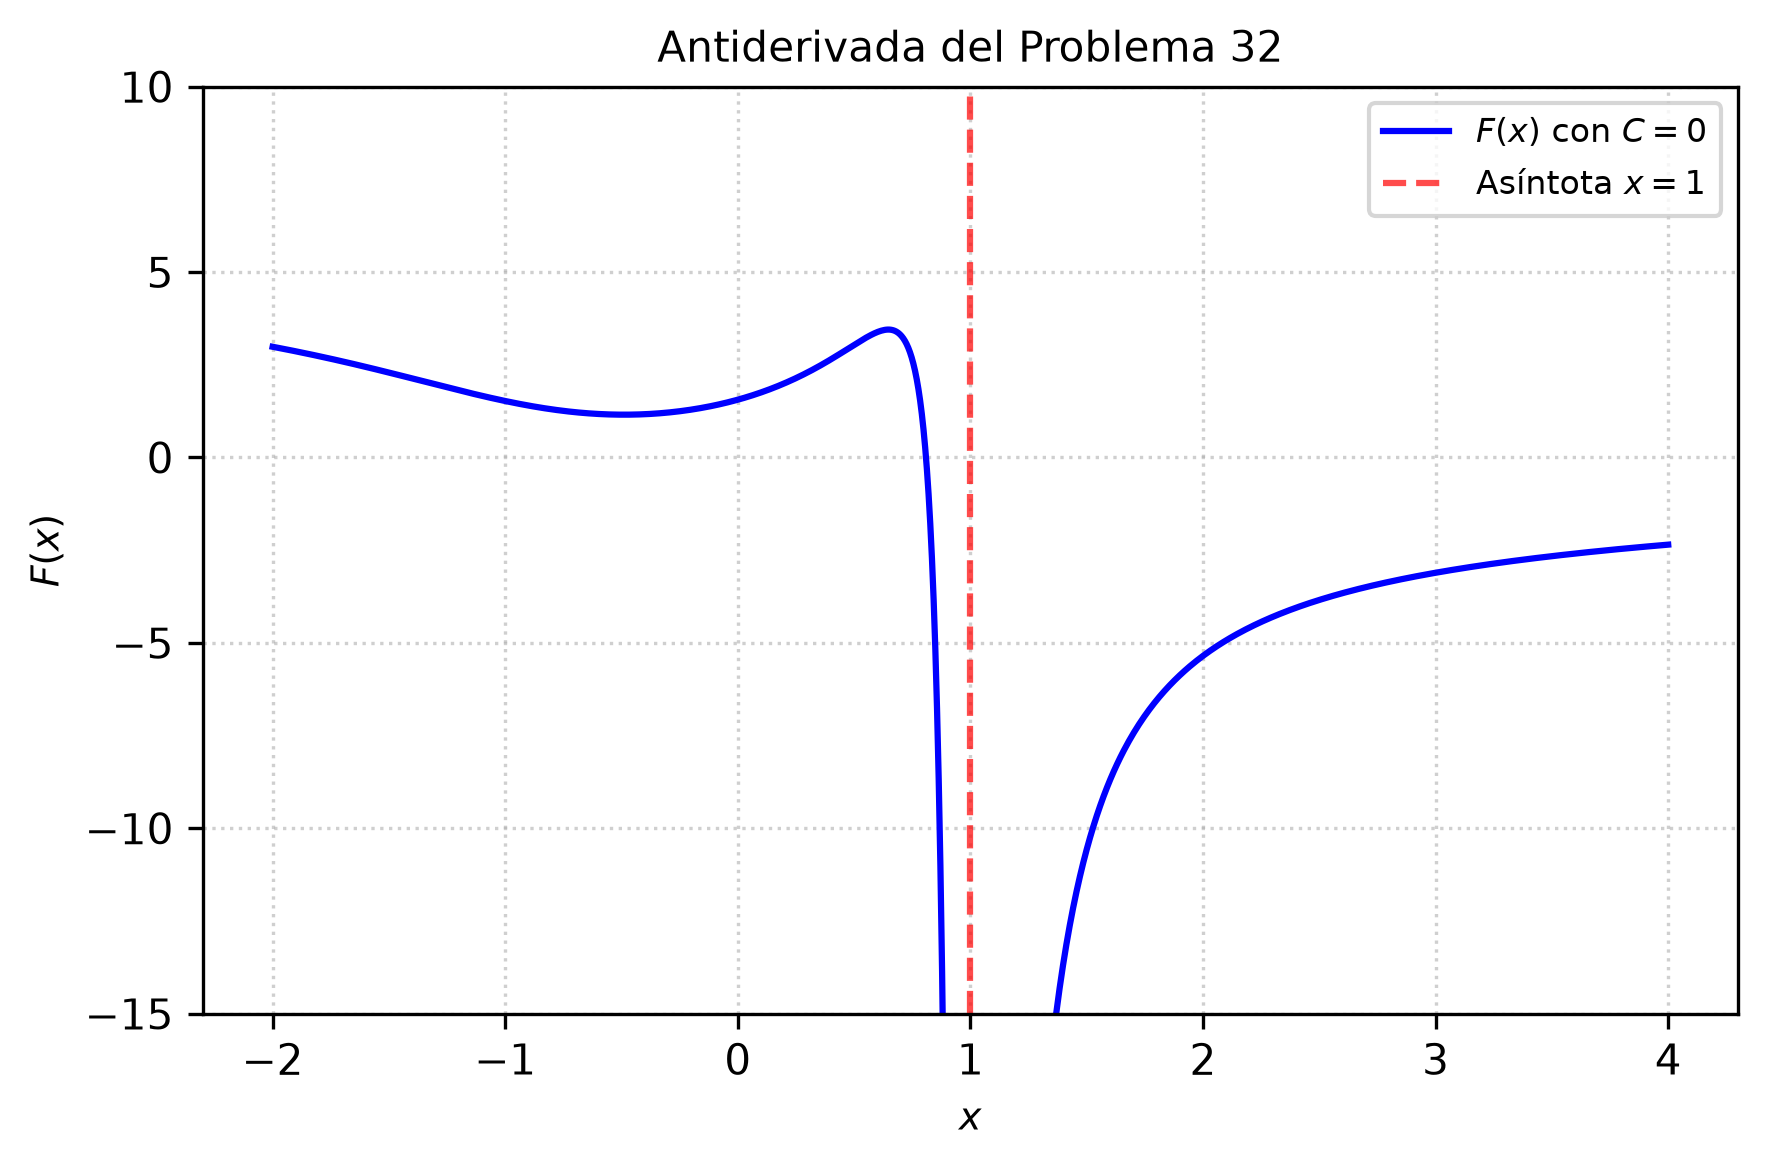
\includegraphics[width=\columnwidth]{semana_03/graficas/SEM03_P32_grafica.png}
	\caption{Representación gráfica de $f(x)$ y su antiderivada $F(x)$ evaluada para la constante de integración $C = 0$ (Problema 32).}
	\label{fig:problema32}
\end{figure}

	\subsection*{Problema 33}
\textbf{Enunciado:} Calcular la integral:
\begin{equation*}
\int \dfrac{4x^4 - 2x^3 - x^2 + 3x + 1}{x^3 + x^2 - x - 1} \, dx
\end{equation*}

\textbf{Solución:} 
Primero, observemos que el grado del numerador es $4$ y el del denominador es $3$. Dado que el grado del numerador es mayor, realizamos la división polinómica. Dividiendo el numerador entre el denominador, obtenemos un cociente y un residuo:

\begin{align*}
\dfrac{4x^4 - 2x^3 - x^2 + 3x + 1}{x^3 + x^2 - x - 1} = \\
4x - 6 + \dfrac{9x^2 + 7x - 5}{x^3 + x^2 - x - 1}
\end{align*}

Ahora factorizamos el denominador agrupando términos:
\begin{align*}
x^3 + x^2 - x - 1 &= x^2(x + 1) - (x + 1) \\
&= (x^2 - 1)(x + 1) \\
&= (x + 1)^2(x - 1)
\end{align*}

Aplicamos fracciones parciales a la expresión restante:
\begin{align*}
\dfrac{9x^2 + 7x - 5}{(x + 1)^2(x - 1)} = \dfrac{A}{x + 1} + \dfrac{B}{(x + 1)^2} + \dfrac{C}{x - 1}
\end{align*}

Multiplicando por el denominador común:
\begin{align*}
9x^2 + 7x - 5 = &A(x + 1)(x - 1) \\
&+ B(x - 1) + C(x + 1)^2
\end{align*}

Evaluando en valores convenientes de $x$:
\begin{itemize}
    \item Si $x = 1$: $11 = 4C \implies C = \dfrac{11}{4}$
    \item Si $x = -1$: $-3 = -2B \implies B = \dfrac{3}{2}$
    \item Si $x = 0$: $-5 = -A - B + C$ \\
    $\implies A = 5 - \dfrac{3}{2} + \dfrac{11}{4} = \dfrac{25}{4}$
\end{itemize}

Sustituyendo los valores hallados, reescribimos la integral completa:
\begin{align*}
\int &\left( 4x - 6 + \dfrac{25/4}{x + 1} + \dfrac{3/2}{(x + 1)^2} + \dfrac{11/4}{x - 1} \right) dx
\end{align*}

Integramos término a término:
\begin{align*}
&= 2x^2 - 6x + \dfrac{25}{4}\ln|x + 1| \\
&\quad - \dfrac{3}{2(x + 1)} + \dfrac{11}{4}\ln|x - 1| + C
\end{align*}

\begin{figure}[H]
	\centering
	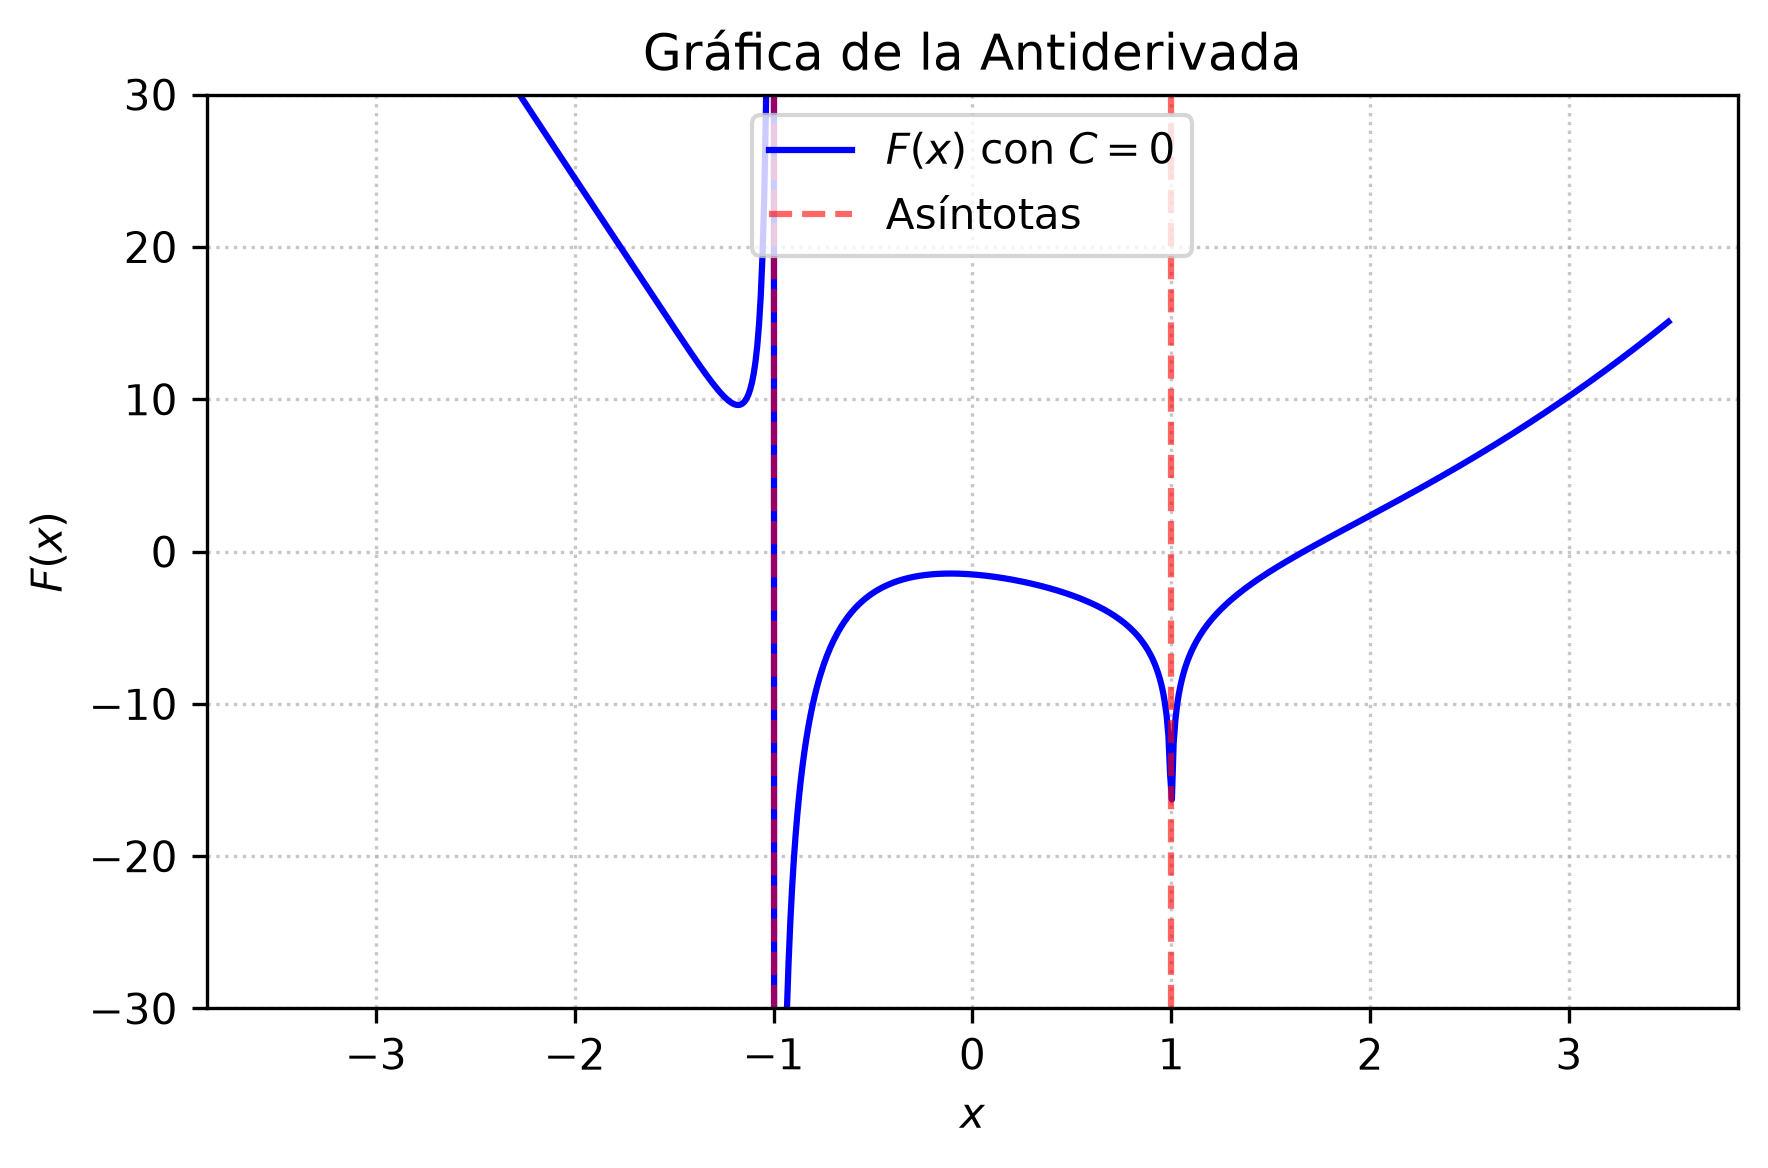
\includegraphics[width=\columnwidth]{semana_03/graficas/SEM03_P33_grafica.png}
	\caption{Representación gráfica de $f(x)$ y su antiderivada $F(x)$ evaluada para la constante de integración $C = 0$ (Problema 33).}
	\label{fig:problema33}
\end{figure}

	\subsection*{Problema 34}

\textbf{Enunciado:} \\
Calcular la integral indefinida:
\begin{align*}
\int \dfrac{3x^4}{(x^2 + 1)^2} \, dx
\end{align*}

\textbf{Solución:} \\
Para resolver esta integral, podemos reescribir el numerador en términos de factores de $(x^2 + 1)$ para simplificar la fracción algebraica sin recurrir directamente a la sustitución trigonométrica.

Primero, expandimos el numerador manipulando algebraicamente $x^4$:
\begin{align*}
3x^4 &= 3(x^2 + 1 - 1)^2 \\
&= 3\left[(x^2 + 1)^2 - 2(x^2 + 1) + 1\right]
\end{align*}

Sustituimos esta expresión de vuelta en el integrando original:
\begin{align*}
&\int \dfrac{3x^4}{(x^2 + 1)^2} \, dx = \\
&\int \dfrac{3\left[(x^2 + 1)^2 - 2(x^2 + 1) + 1\right]}{(x^2 + 1)^2} \, dx
\end{align*}

dividimos cada término del numerador entre el denominador común $(x^2 + 1)^2$:
\begin{align*}
= 3 \int \left[ 1 - \dfrac{2}{x^2 + 1} + \dfrac{1}{(x^2 + 1)^2} \right] dx
\end{align*}

integramos término a término:
\begin{align*}
= 3 \int 1 \, dx &- 6 \int \dfrac{1}{x^2 + 1} \, dx \\
&+ 3 \int \dfrac{1}{(x^2 + 1)^2} \, dx
\end{align*}

Las primeras dos integrales son inmediatas:
\begin{align*}
3 \int 1 \, dx &= 3x \\
-6 \int \dfrac{1}{x^2 + 1} \, dx &= -6 \arctan(x)
\end{align*}

Para la tercera integral, $\int \dfrac{1}{(x^2 + 1)^2} \, dx$, utilizamos la sustitución trigonométrica $x = \tan(\theta)$, de donde $dx = \sec^2(\theta) \, d\theta$:
\begin{align*}
\int \dfrac{\sec^2(\theta)}{(\tan^2(\theta) + 1)^2} \, d\theta &= \int \dfrac{\sec^2(\theta)}{(\sec^2(\theta))^2} \, d\theta \\
&= \int \dfrac{1}{\sec^2(\theta)} \, d\theta \\
&= \int \cos^2(\theta) \, d\theta
\end{align*}

Usando la identidad del ángulo doble:
\begin{align*}
\int \dfrac{1 + \cos(2\theta)}{2} \, d\theta &= \dfrac{\theta}{2} + \dfrac{\sin(2\theta)}{4} \\
&= \dfrac{\theta}{2} + \dfrac{\sin(\theta)\cos(\theta)}{2}
\end{align*}

Regresando a la variable original $x$:
\begin{align*}
\theta &= \arctan(x), \\
\sin(\theta) &= \dfrac{x}{\sqrt{x^2 + 1}}, \quad \cos(\theta) = \dfrac{1}{\sqrt{x^2 + 1}}
\end{align*}

Por lo tanto, la tercera integral resulta en:
\begin{align*}
\dfrac{\arctan(x)}{2} + \dfrac{x}{2(x^2 + 1)}
\end{align*}

Multiplicando por el factor 3 externo:
\begin{align*}
3 \left( \dfrac{\arctan(x)}{2} + \dfrac{x}{2(x^2 + 1)} \right) = \dfrac{3}{2}\arctan(x) + \dfrac{3x}{2(x^2 + 1)}
\end{align*}

Agrupando todos los resultados parciales y añadiendo la constante de integración $C$:
\begin{align*}
3x &- 6\arctan(x) \\
&+ \dfrac{3}{2}\arctan(x) + \dfrac{3x}{2(x^2 + 1)} + C
\end{align*}

Simplificando los términos semejantes de $\arctan(x)$:
\begin{align*}
-6\arctan(x) + \dfrac{3}{2}\arctan(x) = -\dfrac{9}{2}\arctan(x)
\end{align*}

Finalmente, la solución general es:
\begin{align*}
3x - \dfrac{9}{2}\arctan(x) + \dfrac{3x}{2(x^2 + 1)} + C
\end{align*}

\begin{figure}[H]
	\centering
	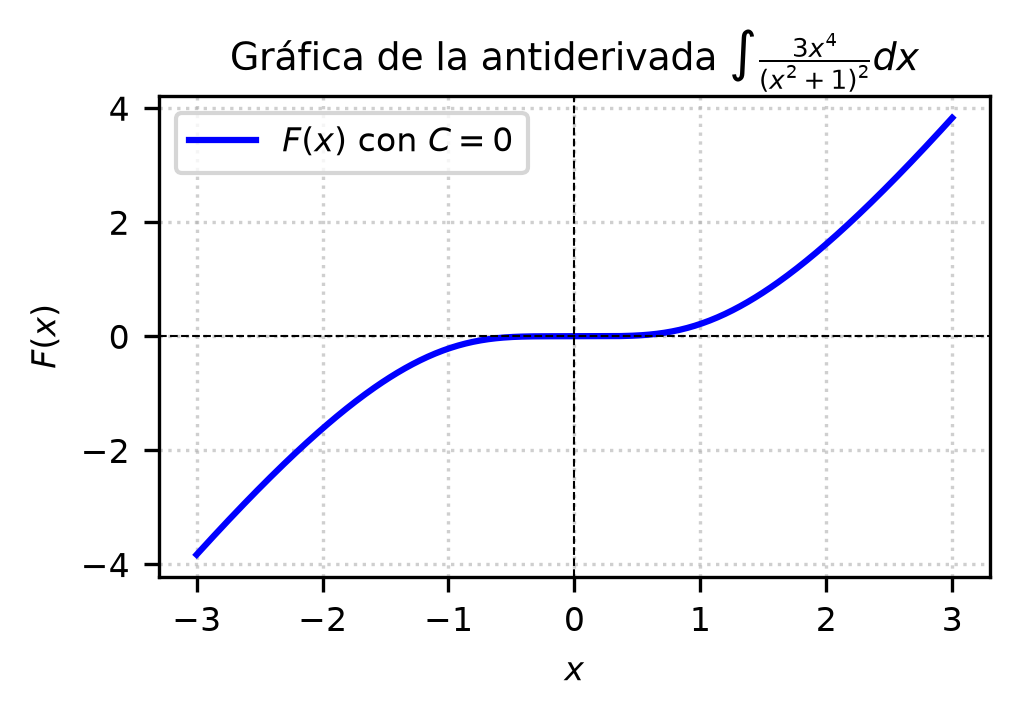
\includegraphics[width=\columnwidth]{semana_03/graficas/SEM03_P34_grafica.png}
	\caption{Representación gráfica de $f(x)$ y su antiderivada $F(x)$ evaluada para la constante de integración $C = 0$ (Problema 34).}
	\label{fig:problema34}
\end{figure}

	\subsection*{Problema 35}

\textbf{Enunciado:}
Calcular la integral indefinida:
\begin{equation*}
\int \dfrac{2x^2 + 41x - 91}{x^3 - 2x^2 - 11x + 12} \, dx
\end{equation*}

\textbf{Solución:}
El denominador se puede factorizar como se indica en las observaciones:
\begin{equation*}
x^3 - 2x^2 - 11x + 12 = (x - 1)(x - 4)(x + 3)
\end{equation*}

Planteamos la descomposición en fracciones simples para el integrando:
\begin{multline*}
\dfrac{2x^2 + 41x - 91}{(x - 1)(x - 4)(x + 3)} = \\
\dfrac{A}{x - 1} + \dfrac{B}{x - 4} + \dfrac{C}{x + 3}
\end{multline*}

Multiplicando ambos lados por el denominador común, obtenemos:
\begin{multline*}
2x^2 + 41x - 91 = A(x - 4)(x + 3) \\
+ B(x - 1)(x + 3) + C(x - 1)(x - 4)
\end{multline*}

Evaluamos en los valores críticos para hallar las constantes:
\begin{align*}
\text{Si } x &= 1: \\
2(1)^2 + 41(1) - 91 &= A(1 - 4)(1 + 3) \\
-48 &= -12A \implies A = 4 \\
\text{Si } x &= 4: \\
2(4)^2 + 41(4) - 91 &= B(4 - 1)(4 + 3) \\
84 &= 21B \implies B = 4 \\
\text{Si } x &= -3: \\
2(-3)^2 + 41(-3) - 91 &= C(-3 - 1)(-3 - 4) \\
-196 &= 28C \implies C = -7
\end{align*}

Sustituyendo los valores de $A$, $B$ y $C$ en la integral:
\begin{multline*}
\int \dfrac{2x^2 + 41x - 91}{x^3 - 2x^2 - 11x + 12} \, dx = \\
\int \left( \dfrac{4}{x - 1} + \dfrac{4}{x - 4} - \dfrac{7}{x + 3} \right) dx
\end{multline*}

Integramos cada término de forma directa utilizando logaritmos:
\begin{align*}
\int \dfrac{4}{x - 1} \, dx &= 4 \ln|x - 1| \\
\int \dfrac{4}{x - 4} \, dx &= 4 \ln|x - 4| \\
\int \dfrac{7}{x + 3} \, dx &= 7 \ln|x + 3|
\end{align*}

Agrupando los resultados y aplicando propiedades de logaritmos, la solución general es:
\begin{multline*}
= 4 \ln|x - 1| + 4 \ln|x - 4| \\
- 7 \ln|x + 3| + C
\end{multline*}
O de forma compacta:
\begin{equation*}
= \ln\left( \dfrac{(x - 1)^4 (x - 4)^4}{(x + 3)^7} \right) + C
\end{equation*}

\begin{figure}[H]
	\centering
	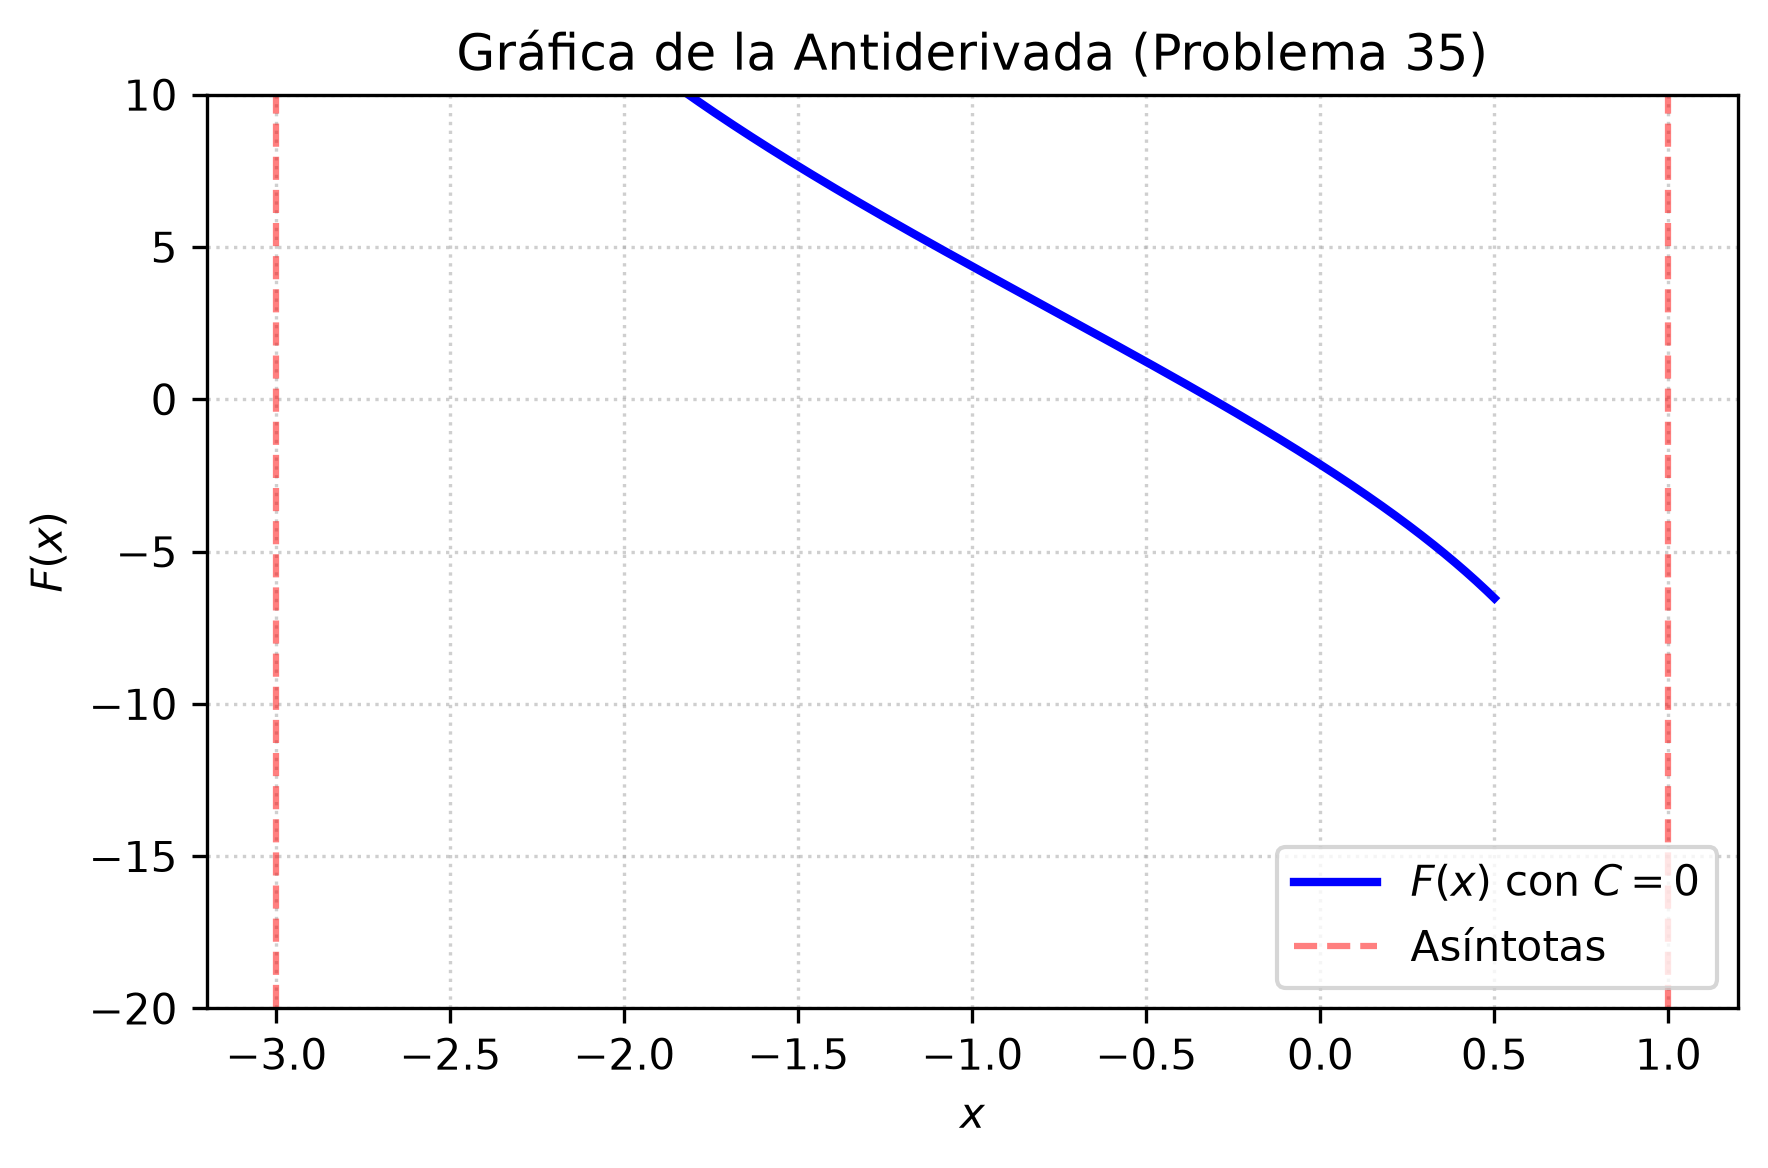
\includegraphics[width=\columnwidth]{semana_03/graficas/SEM03_P35_grafica.png}
	\caption{Representación gráfica de $f(x)$ y su antiderivada $F(x)$ evaluada para la constante de integración $C = 0$ (Problema 35).}
	\label{fig:problema35}
\end{figure}

	\subsection*{Problema 36}

\textbf{Enunciado:}
Calcular la integral indefinida:
\begin{align*}
\int \dfrac{2x^4 + 3x^3 - x - 1}{(x - 1)(x^2 + 2x + 2)^2} \, dx
\end{align*}

\textbf{Solución:}
El integrando es una función racional propia. 
Utilizamos el método de fracciones parciales 
con la descomposición indicada:

\begin{align*}
\dfrac{2x^4 + 3x^3 - x - 1}{(x - 1)(x^2 + 2x + 2)^2} &= 
\dfrac{A}{x - 1} \\
&+ \dfrac{Bx + C}{x^2 + 2x + 2} \\
&+ \dfrac{Dx + E}{(x^2 + 2x + 2)^2}
\end{align*}

Multiplicando ambos lados por el denominador 
común, obtenemos la identidad polinómica. 
Evaluando en $x = 1$, determinamos el coeficiente:
\begin{align*}
A &= \dfrac{2(1)^4 + 3(1)^3 - 1 - 1}{(1^2 + 2(1) + 2)^2} \\
&= \dfrac{3}{5^2} = \dfrac{3}{25}
\end{align*}

Expandiendo y agrupando términos semejantes para 
los coeficientes restantes, hallamos:
\begin{align*}
B &= \dfrac{47}{25}, \quad C = -\dfrac{4}{25} \\
D &= \dfrac{3}{5}, \quad E = -\dfrac{1}{5}
\end{align*}

Sustituyendo los valores, la integral se 
descompone en tres partes:
\begin{align*}
\int \dfrac{3/25}{x - 1} \, dx 
&+ \int \dfrac{\frac{47}{25}x - \frac{4}{25}}{x^2 + 2x + 2} \, dx \\
&+ \int \dfrac{\frac{3}{5}x - \frac{1}{5}}{(x^2 + 2x + 2)^2} \, dx
\end{align*}

La primera integral es inmediata:
\begin{align*}
\int \dfrac{3/25}{x - 1} \, dx = \dfrac{3}{25} \ln|x - 1|
\end{align*}

Para la segunda integral, reescribimos el 
numerador usando la derivada del denominador 
$2x + 2$:
\begin{align*}
\dfrac{47}{50} \int \dfrac{2x + 2}{x^2 + 2x + 2} \, dx 
- \dfrac{107}{50} \int \dfrac{1}{(x + 1)^2 + 1} \, dx
\end{align*}
Esto resulta en:
\begin{align*}
\dfrac{47}{50} \ln(x^2 + 2x + 2) - \dfrac{107}{50} \arctan(x + 1)
\end{align*}

Para la tercera integral, aplicamos la 
sustitución trigonométrica $x + 1 = \tan(\theta)$, 
con lo cual $dx = \sec^2(\theta) \, d\theta$:
\begin{align*}
\int \dfrac{\frac{3}{5}(\tan\theta - 1)}{\sec^4(\theta)} \sec^2(\theta) \, d\theta 
&= \dfrac{3}{5} \int \dfrac{\sin\theta - \cos\theta}{\sec^2(\theta)} \, d\theta \\
&= -\dfrac{3}{10}\cos^2\theta - \dfrac{3}{10}(\theta + \sin\theta\cos\theta)
\end{align*}

Retornando a la variable original $x$ y 
sumando todas las antiderivadas, obtenemos 
la solución general con $C$ como constante de integración:
\begin{align*}
F(x) &= \dfrac{3}{25}\ln|x - 1| 
+ \dfrac{47}{50}\ln(x^2 + 2x + 2) \\
&- \dfrac{107}{50}\arctan(x + 1) \\
&- \dfrac{3}{5(x^2 + 2x + 2)} + C
\end{align*}

\begin{figure}[H]
	\centering
	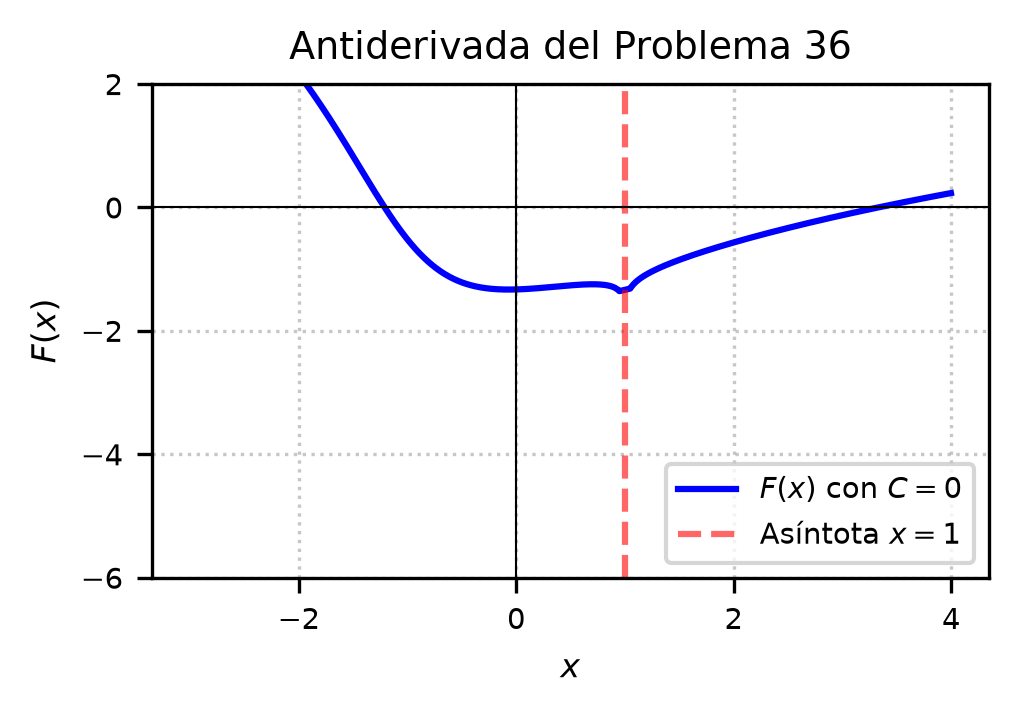
\includegraphics[width=\columnwidth]{semana_03/graficas/SEM03_P36_grafica.png}
	\caption{Representación gráfica de $f(x)$ y su antiderivada $F(x)$ evaluada para la constante de integración $C = 0$ (Problema 36).}
	\label{fig:problema36}
\end{figure}

	\subsection*{Problema 37}
\textbf{Enunciado:} Calcular la integral:
\begin{align*}
\int \dfrac{5x^3 + 2}{x^3 - 5x^2 + 4x} \, dx
\end{align*}

\textbf{Solución:} 
Dado que el grado del numerador es igual al grado del denominador, realizamos la división polinómica de la función integrando:
\begin{align*}
\dfrac{5x^3 + 2}{x^3 - 5x^2 + 4x} = 5 + \dfrac{25x^2 - 20x + 2}{x^3 - 5x^2 + 4x}
\end{align*}

El denominador se factoriza como:
\begin{align*}
x^3 - 5x^2 + 4x = x(x - 1)(x - 4)
\end{align*}

Aplicamos fracciones parciales a la parte racional restante:
\begin{align*}
\dfrac{25x^2 - 20x + 2}{x(x - 1)(x - 4)} = \dfrac{A}{x} + \dfrac{B}{x - 1} + \dfrac{C}{x - 4}
\end{align*}

Multiplicando por el denominador común:
\begin{align*}
25x^2 - 20x + 2 &= A(x-1)(x-4) \\
&\quad + Bx(x-4) + Cx(x-1)
\end{align*}

Evaluando en valores convenientes de $x$:
\begin{align*}
x = 0 &\implies 2 = 4A \implies A = \dfrac{1}{2} \\
x = 1 &\implies 7 = -3B \implies B = -\dfrac{7}{3} \\
x = 4 &\implies 322 = 12C \implies C = \dfrac{161}{6}
\end{align*}

Sustituyendo los valores hallados y el cociente de la división en la integral original:
\begin{align*}
\int &\left( 5 + \dfrac{1/2}{x} - \dfrac{7/3}{x - 1} + \dfrac{161/6}{x - 4} \right) dx
\end{align*}

Integramos cada término por separado:
\begin{align*}
&= 5x + \dfrac{1}{2}\ln|x| - \dfrac{7}{3}\ln|x - 1| \\
&\quad + \dfrac{161}{6}\ln|x - 4| + C
\end{align*}

\begin{figure}[H]
	\centering
	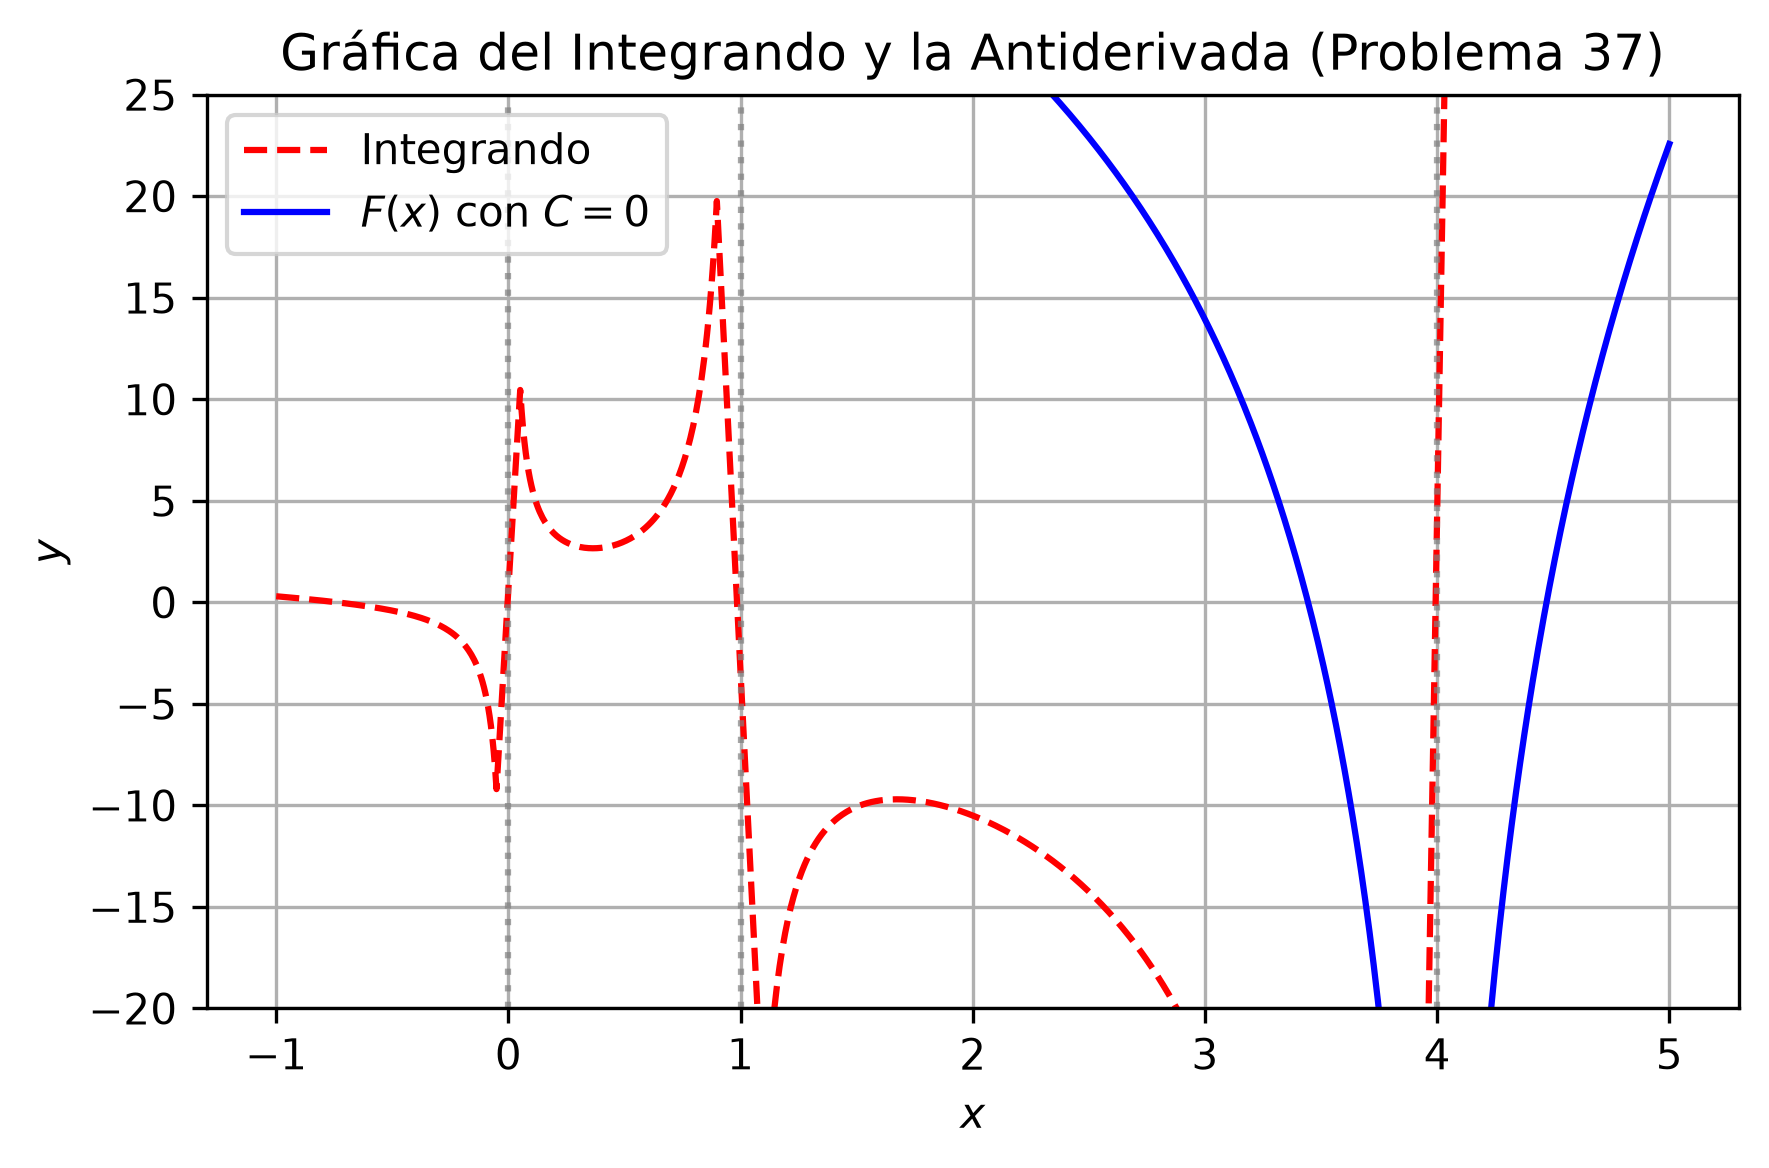
\includegraphics[width=\columnwidth]{semana_03/graficas/SEM03_P37_grafica.png}
	\caption{Representación gráfica de $f(x)$ y su antiderivada $F(x)$ evaluada para la constante de integración $C = 0$ (Problema 37).}
	\label{fig:problema37}
\end{figure}

	\subsection*{Problema 38}

\textbf{Enunciado:} 
Calcular la integral indefinida:
\begin{align*}
I = \int \dfrac{x^5}{(x^3 + 1)(x^3 + 8)} \, dx
\end{align*}

\textbf{Solución:}
Siguiendo la indicación, realizamos el cambio de variable:
\begin{align*}
u &= x^3, \quad du = 3x^2 \, dx \\
\dfrac{du}{3} &= x^2 \, dx
\end{align*}

Reescribimos el integrando para hacer visible el término $x^2 \, dx$:
\begin{align*}
I &= \int \dfrac{x^3 \cdot x^2}{(x^3 + 1)(x^3 + 8)} \, dx \\
I &= \int \dfrac{u}{(u + 1)(u + 8)} \left(\dfrac{du}{3}\right) \\
I &= \dfrac{1}{3} \int \dfrac{u}{(u + 1)(u + 8)} \, du
\end{align*}

Aplicamos descomposición en fracciones parciales al integrando en la variable $u$:
\begin{align*}
\dfrac{u}{(u + 1)(u + 8)} &= \dfrac{A}{u + 1} + \dfrac{B}{u + 8}
\end{align*}

Multiplicando por el denominador común:
\begin{align*}
u &= A(u + 8) + B(u + 1)
\end{align*}

Evaluando para $u = -1$:
\begin{align*}
-1 &= A(-1 + 8) \implies 7A = -1 \implies A = -\dfrac{1}{7}
\end{align*}

Evaluando para $u = -8$:
\begin{align*}
-8 &= B(-8 + 1) \implies -7B = -8 \implies B = \dfrac{8}{7}
\end{align*}

Sustituimos las constantes en la integral:
\begin{align*}
I &= \dfrac{1}{3} \int \left( \dfrac{-1/7}{u + 1} + \dfrac{8/7}{u + 8} \right) du \\
I &= \dfrac{1}{21} \int \left( -\dfrac{1}{u + 1} + \dfrac{8}{u + 8} \right) du
\end{align*}

Integramos cada término respecto a $u$:
\begin{align*}
I &= \dfrac{1}{21} \left( -\ln|u + 1| + 8\ln|u + 8| \right) + C
\end{align*}

Regresando a la variable original $x$ mediante $u = x^3$:
\begin{align*}
I &= \dfrac{1}{21} \left( 8\ln|x^3 + 8| - \ln|x^3 + 1| \right) + C
\end{align*}

Por lo tanto, la solución general es:
\begin{align*}
I &= \dfrac{1}{21} \ln\left| \dfrac{(x^3 + 8)^8}{x^3 + 1} \right| + C
\end{align*}

\begin{figure}[H]
	\centering
	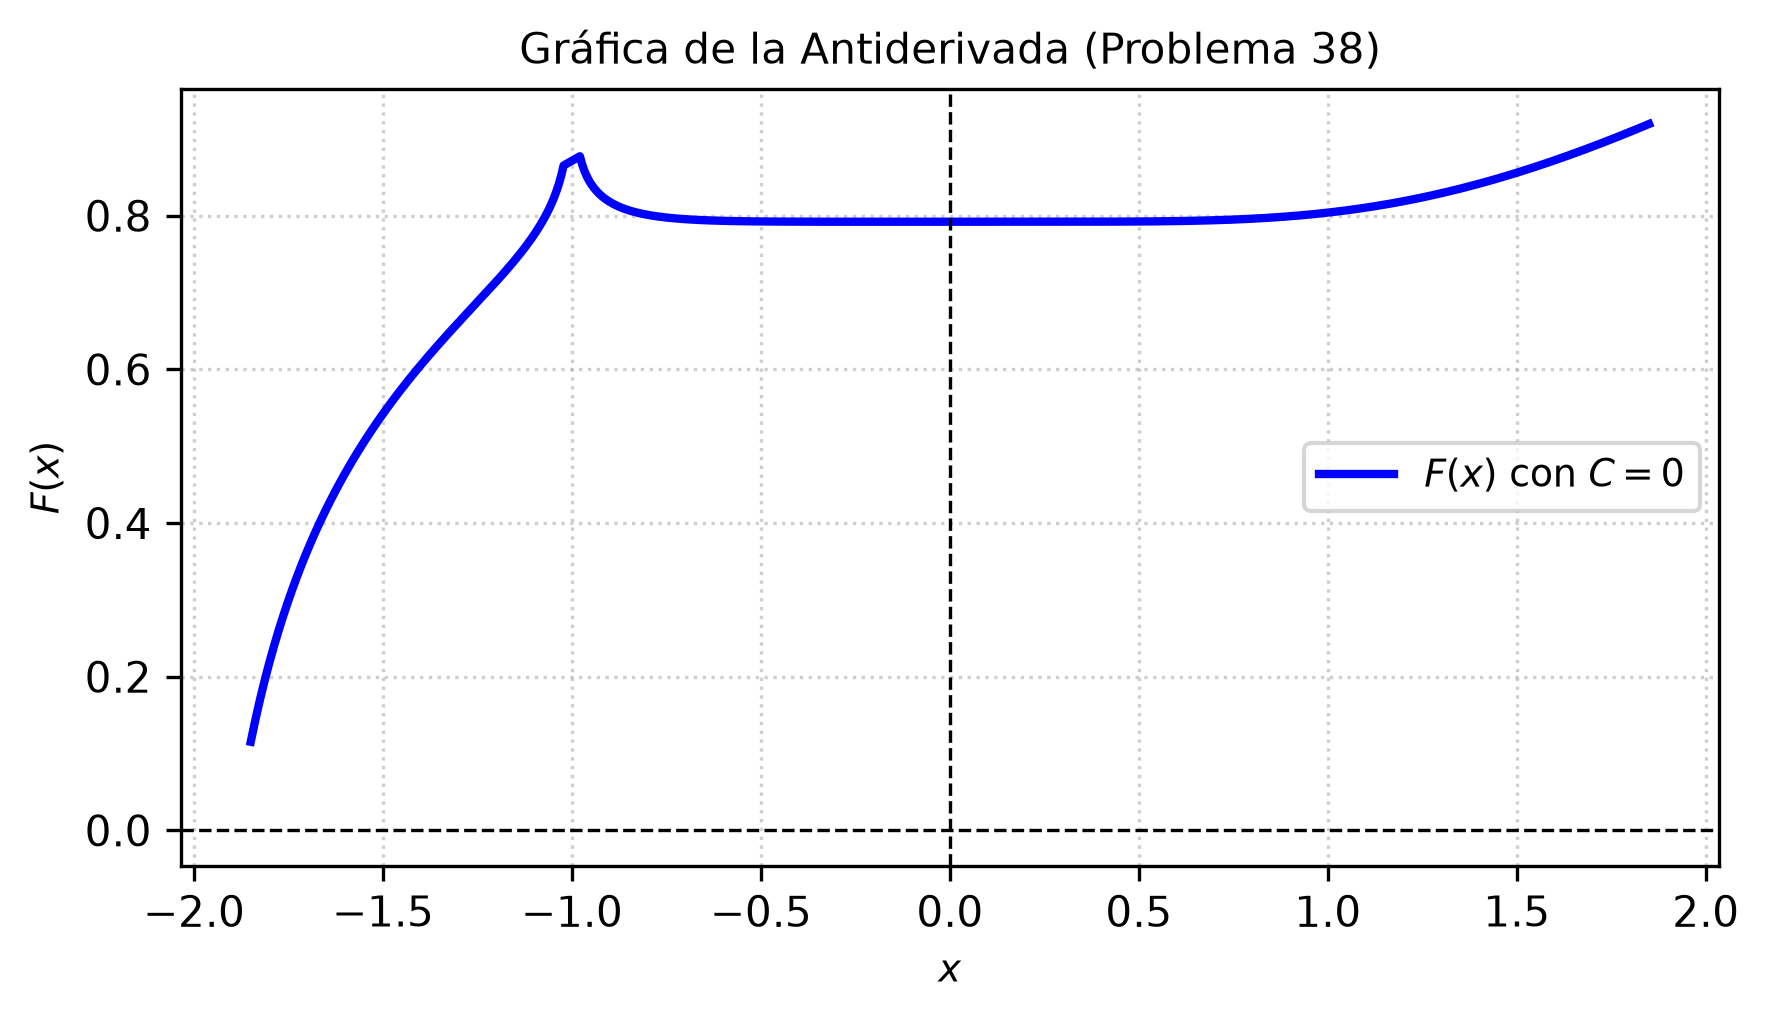
\includegraphics[width=\columnwidth]{semana_03/graficas/SEM03_P38_grafica.png}
	\caption{Representación gráfica de $f(x)$ y su antiderivada $F(x)$ evaluada para la constante de integración $C = 0$ (Problema 38).}
	\label{fig:problema38}
\end{figure}

	%\input{semana_03/tex_soluciones/SEM03_P39_solucion.tex}
	%\input{semana_03/tex_soluciones/SEM03_P40_solucion.tex}
	%\input{semana_03/tex_soluciones/SEM03_P41_solucion.tex}
	%\input{semana_03/tex_soluciones/SEM03_P42_solucion.tex}
	%\input{semana_03/tex_soluciones/SEM03_P43_solucion.tex}
	%\input{semana_03/tex_soluciones/SEM03_P44_solucion.tex}
	%\input{semana_03/tex_soluciones/SEM03_P45_solucion.tex}
	%\input{semana_03/tex_soluciones/SEM03_P46_solucion.tex}
	%\input{semana_03/tex_soluciones/SEM03_P47_solucion.tex}
	%\input{semana_03/tex_soluciones/SEM03_P48_solucion.tex}
	%\input{semana_03/tex_soluciones/SEM03_P49_solucion.tex}
	%\input{semana_03/tex_soluciones/SEM03_P50_solucion.tex}
	%\input{semana_03/tex_soluciones/SEM03_P51_solucion.tex}
	%\input{semana_03/tex_soluciones/SEM03_P52_solucion.tex}
	%\input{semana_03/tex_soluciones/SEM03_P53_solucion.tex}
	%\input{semana_03/tex_soluciones/SEM03_P54_solucion.tex}
	%\input{semana_03/tex_soluciones/SEM03_P55_solucion.tex}
	%\input{semana_03/tex_soluciones/SEM03_P56_solucion.tex}
	%\input{semana_03/tex_soluciones/SEM03_P57_solucion.tex}
	%\input{semana_03/tex_soluciones/SEM03_P58_solucion.tex}
	%\input{semana_03/tex_soluciones/SEM03_P59_solucion.tex}
	%\input{semana_03/tex_soluciones/SEM03_P60_solucion.tex}
	%\input{semana_03/tex_soluciones/SEM03_P61_solucion.tex}
	%\input{semana_03/tex_soluciones/SEM03_P62_solucion.tex}
	%\input{semana_03/tex_soluciones/SEM03_P63_solucion.tex}
	%\input{semana_03/tex_soluciones/SEM03_P64_solucion.tex}
	%\input{semana_03/tex_soluciones/SEM03_P65_solucion.tex}
	%\input{semana_03/tex_soluciones/SEM03_P66_solucion.tex}
	%\input{semana_03/tex_soluciones/SEM03_P67_solucion.tex}
	%\input{semana_03/tex_soluciones/SEM03_P68_solucion.tex}
	%\input{semana_03/tex_soluciones/SEM03_P69_solucion.tex}
	%\input{semana_03/tex_soluciones/SEM03_P70_solucion.tex}
	%\input{semana_03/tex_soluciones/SEM03_P71_solucion.tex}
	%\input{semana_03/tex_soluciones/SEM03_P72_solucion.tex}
	%\input{semana_03/tex_soluciones/SEM03_P73_solucion.tex}
	%\input{semana_03/tex_soluciones/SEM03_P74_solucion.tex}
	%\input{semana_03/tex_soluciones/SEM03_P75_solucion.tex}
	%\input{semana_03/tex_soluciones/SEM03_P76_solucion.tex}
	%\input{semana_03/tex_soluciones/SEM03_P77_solucion.tex}
	%\input{semana_03/tex_soluciones/SEM03_P78_solucion.tex}
	%\input{semana_03/tex_soluciones/SEM03_P79_solucion.tex}
	%\input{semana_03/tex_soluciones/SEM03_P80_solucion.tex}
	
\end{document}